\providecommand{\classoptions}{keys}
\documentclass[noworkareas,deliverables,\classoptions]{euproposal}       % for writing
%\documentclass[submit,noworkareas,deliverables]{euproposal}        % for submission
%\documentclass[submit,public,noworkareas,deliverables]{euproposal} % for public version

\usepackage[utf8]{inputenc}
%\usepackage{minitoc}

\usepackage{float}  % used to suppress floating of tables in Resources section.
\usetikzlibrary{calc,fit,positioning,shapes,arrows,snakes}

\addbibresource{kwarc.bib}
\addbibresource{bibliography.bib}
% temporary fix due to http://tex.stackexchange.com/questions/311426/bibliography-error-use-of-blxbblverbaddi-doesnt-match-its-definition-ve
\makeatletter\def\blx@maxline{77}\makeatother

\WAperson[id=miko, 
           personaltitle=Prof. Dr.,
           birthdate=13. September 1964,
           academictitle=Professor of Computer Science,
           affiliation=jacu,
           department=case,
           privaddress=None of your business,
           privtel=that neither,
           email=m.kohlhase@jacobs-university.de,
           workaddress={Campus Ring 1, 28757 Bremen},
           worktel=+49 421 200 3140,
           worktelfax=+49 421 200 3140/493140,
           workfax=+49 421 200 493140]
           {Michael Kohlhase}
\WAperson[id=gc,
           personaltitle=Dr.,
           academictitle=Senior Researcher,
           birthdate=14. April 1972,
           affiliation=pcg,
           department=pcsa,
           privaddress=None of your business,
           privtel=that neither,
           workaddress= ,
           worktel=+49 421 0815 4711,
           workfax=+49 421 0815 4712,
           email=gc@pcg.phony]
           {Great Communicator}

\WAinstitution[id=case,acronym=CASE,shortname=CASE,
                url=http://jacobs-university.de/ses/case,
                partof=jacu]
               {Center for Advanced Systems Engineering}
\WAinstitution[id=jacu,
               url=http://jacobs-university.de,
               streetaddress={Campus Ring 1},
               townzip={28759 Bremen},
               countryshort=D,
               country=Germany,
               type=University,
               logo=jacobs-logo.png,
               acronym=JACU,
               shortname=Jacobs University]
               {Jacobs University Bremen}

\WAinstitution[id=pcsa,
                           url=http://pcg.phony/sa,
                           partof=pcg]
               {Science Affairs}
\WAinstitution[id=pcg,
                           url=http://pcg.phony,
                           acronym=PCG,
                           shortname=Power Consulting,
                           countryshort=D,
                           streetaddress={Seefahrtstrasse 5},
                           townzip={23555 Hamburg}]
               {Power Consulting GmbH}

\WAinstitution[id=efo,
                           url=http://efo.eu,
                           countryshort=NL,
                           townzip={Utrecht, 3kd89},
                           streetaddress={Kruislann 777},
                           country={The Netherlands},
                           type=NGO,
                           acronym=EFO,
                           shortname=European Future Office]
             {European Future Office}

\WAinstitution[id=bar,
                           url=http://bar.fr,
                           countryshort=F,
                           country={France},
                           streetaddress={Rue de Montparnasse}
                           townzip={Paris},
                           type=University,
                           acronym=BAR,
                           shortname=Universit\'e de BAR]
             {Universit\'e de BAR}

\WAinstitution[id=baz,
                          url=http://baz.co.uk,
                          countryshort=UK,
                          streetaddress={4711 Silicon Glen Drive},
                          townzip={Westerfield U3F2B},
                          type=SME,
                          shortname=BAZ International,
                          acronym=BAZ]
             {BAZ International Ltd}

%%% Local Variables: 
%%% mode: latex
%%% End: 

% LocalWords:  WAperson miko personaltitle academictitle privaddress privtel
% LocalWords:  workaddress worktel workfax gc worktelfax pcg pcsa WAinstitution
% LocalWords:  shortname partof streetaddress townzip countryshort efo 3kd89
% LocalWords:  jacobs-logo.png Seefahrtstrasse Kruislann Montparnasse Universit
% LocalWords:  baz Westerfield
 % Some sections of the included files depend on this.
\usepackage{lscape} % for landscape
\usepackage{comments}
% %\usepackage[final]{comments}
\usepackage{verbatim}
\usepackage{listings}
\usepackage{supertabular,array}
\makeatletter
\newcommand\arraybslash{\let\\\@arraycr}
\makeatother
% \setlength\tabcolsep{1mm}
% \renewcommand\arraystretch{1.3}
%% Related Projects
\newcommand{\scienceproject}{\mbox{\textsc{SCIEnce}}}
\newcommand{\OOMMFNB}{OOMMF-NB}

\newcommand{\software}[1]{\texttt{#1}\xspace}
\newcommand{\GAP}{\software{GAP}}
\newcommand{\libGAP}{\software{libGAP}}
\newcommand{\Singular}{\software{Singular}}
\newcommand{\Sage}{\software{Sage}}
\newcommand{\SageCombinat}{\software{Sage-Combinat}}
\newcommand{\Python}{\software{Python}}
\newcommand{\IPython}{\software{IPython}}
\newcommand{\Jupyter}{\software{Jupyter}}
\newcommand{\Cython}{\software{Cython}}
\newcommand{\Pythran}{\software{Pythran}}
\newcommand{\Numpy}{\software{Numpy}}
\newcommand{\Pari}{\software{PARI}}
\newcommand{\PariGP}{\software{PARI/GP}}
\newcommand{\Linbox}{\software{LinBox}}
\newcommand{\LMFDB}{\software{LMFDB}}
\newcommand{\OpenEdX}{\software{OpenEdX}}
\newcommand{\Linux}{\software{Linux}}
\newcommand{\LATEX}{\software{\LaTeX}}
\newcommand{\SMC}{\software{SageMathCloud}}
\newcommand{\Simulagora}{\software{Simulagora}}
\newcommand{\Magma}{\software{Magma}}
\newcommand{\Mathematica}{\software{Mathematica}}
\newcommand{\Maple}{\software{Maple}}
\newcommand{\Matlab}{\software{Matlab}}
\newcommand{\Arxiv}{\software{arXiv}}

%%% Local Variables: 
%%% mode: latex
%%% TeX-master: "proposal"
%%% End: 

\usepackage{framed}

\begin{document}
\begin{proposal}[
  % These PM numbers (person months) are for the coordinator to help planning
  % Participants should not change these, but add PM numbers in the CVS in
  % the site descriptions at CVs/*.tex
  % TODO: Nicolas needs to update these numbers from the (requested ones)
  site=PS, %paris sud
  site=UB,   % CNRS (Bordeaux)
  site=JU,  % Jacobs University Bremen
  site=UJF, % Univ Josef Fourier Grenoble
  site=UK, % Kaiserslautern
  site=UO, % Oxford
  site=US, % Silesia
  site=USH, % Sheffield
  site=USO, % Southhampton
  site=SA, % St Andrews
  site=UV, % Versailles
  site=UW, % Warwick
  site=ZH, % Z"urich
  site=LL, % logilab
  site=SR, % Simula
  site=UG, % Gent
  site=FAU, % FAU Erlangen/Nuremberg
  botupPM, % we want to work via bottom up PM distribution,
  % alternative: (can be combined)
  % topdownPM, % the coordinator distributes PM as follows:
  % PSRM=48, %paris sud
  % LLRM=48, % logilab
  % UVRM=48, % Versailles
  % UJFRM=48, % Fourier
  % UBRM=48,   % CNRS (Bordeaux)
  % UORM=48, % Oxford
  % USHRM=48, % Sheffieldg
  % USORM=48, % Southhampton
  % SARM=48, % St Andrews
  % UWRM=48, % Warwick
  % JURM=48,  % Jacobs
  % UKRM=48, % Kaiserslautern
  % USRM=48, % Silesia
  % ZHRM=48, % Z"urich
  % SRRM=48, % Simula
    coordinator=thiery,
  coordinatorsite=PS,
  acronym={OpenDreamKit},
  acrolong={OpenDreamKit},
  proposalnumber={676541},
  title=Open Digital Research Environment Toolkit\\ for the Advancement of Mathematics,
  callname=Topic: e-Infrastructures for Virtual Research Environments (VRE),
  callid=EINFRA-9-2015,
  % TODO: consistency with provided template
  % CALL: H2020-EINFRA-2015-1
  % TOPIC: e-Infrastructures for Virtual Research Environments (VRE)
  % Instrument: e-Infrastructures
  keywords={pure mathematics, computer algebra, simulation,
    visualisation, component architecture, databases, 
reproducibility, Sage, IPython, Jupyter, LMFDB, MathHub},
  % computational mathematics,
  % GAP, Linbox, PARI, Sage, Singular, IPython, Jupyter, SageMathCloud, LMFDB, MathHub
  % Virtual research environments, MPIR, /GP
  % open source, free software, number theory, abstract algebra, notebooks
  instrument= Call: H2020-EINFRA-2015-1, %Call: H2020-EINFRA-2015-1, 3 Topic 9-2015
  challengeid = TODO,
  %challenge = {N/A},
  %objectiveid={N/A},
  %objective = TODO,
  %outcomeid = N/A,
  %outcome = N/A,
  coordinator=thiery,
  months=48,
  compactht]
\newcommand{\TheProject}{\pn}% \pn is defined automatically
\ifgrantagreement
\section*{History of changes}

\subsection*{Grant agreement number 676541, June 2015}
\thispagestyle{empty}

\begin{enumerate}
\item Updated participant acronyms for consistency with the EU portal.

\item Resources for UPSud: reinstated PhD position that was planned in
  the budget but went missing in the proposal document: +36PM for UPSud.
\item Reinstated related task T6.5 ``Knowledge-based code infrastructure''.
  +33PM for WP6
\item Minor update to the involvement for Pons, Hivert, Lelièvre at
  UPSud for consistency with the submitted budget (-1PM each).
\item Minor update to the involvement for Gouarin at CNRS to make up
  for a higher salary than expected (-1PM); adapted accordingly WP2
  (-1PM).
\item Where relevant: updated PM information according to the above.

\item WP2: Added mention of our participation to the European
  E-Infrastructure concertation activities.

\item Updated resources to be committed: audit costs should be in the
  direct costs, not subcontracting.

\item Updated the risk table to address the reviewers comments.

\item As suggested by the project officer, reduction of the number of
  deliverables (typically by merging together intermediate
  check-points into the corresponding final deliverable):
  \begin{itemize}
  \item Suppressed irrelevant D1.1. (Consortium agreement).
  \item Removed accidently duplicated deliverables:
    \begin{itemize}
    \item D2.10 Course material on using OpenDreamKit in data science;
    \item D2.12, D2.13 indexing service;
    \item D2.20 Demonstrator: Interactive lecture notes and marking
      systems based on OpenDreamKit.
    \end{itemize}
  \item Merged together D1.5 and D1.8 (Data Management Plan V2,V3)
  \item Merged D2.2, D2.7, D2.14, D2.19, D2.25, and D2.26 (community
    building reports: impact of development and training workshops)
    into a single yearly report.
  \item Merged together D2.3, D2.15, D2.23, and D2.24 (Demonstrators:
    Problems in Physics with Sage v1,2 , Computational Mathematics for
    Engineering).
  \item Merged together D2.8 (Community-curated indexing tool (open
    source)) and D2.9 (Community-curated indexing service for
    OpenDreamKit).
  \item Merged D2.16 (Micromagnetic VRE code and documents source
    online), D3.4 (Python interface to OOMMF completed), D4.8
    (Micromagnetic VRE software completed), D4.11 (Micromagnetic VRE
    tutorial and documentation notebooks), and D4.14 (Demonstrator
    online portal available) into a single deliverable D2.13
    (Micromagnetic VRE completed and online).
  \item Merged D3.1 and D3.9 (one-click install Sage distribution for
    Windows with Cygwin 32bit/64bit).
  \item Merged D5.1 (Facility to compile \Pythran compliant user
    kernels and sage code) and D5.3 (Improve \Pythran runtime support
    to automatically take advantage of multi-cores and SIMD
    instruction units and use it in CYTHON); also switched lead info
    for D5.3 and D5.5 (Improve PYTHRAN typing to improve error
    information).
  \item Merged D5.9 (Report on development of designs for the GAP
    developments – parallel library, interacts to standard
    infrastructure and CYTHON-like extensions) and D5.15
    (Implementations of the GAP developments, ready for release) into
    D5.18 (Final report and evaluation of the GAP developments).
  \item Merged D6.1 (DKS base survey and Requirements Workshop Report)
    and D6.3 (initial DKS base Design).
  \item Merged D6.4 (Design of Triform (DKS) Theories
    (Specification/RNC Schema/Examples)) and D6.5 (Implementation of
    Triform Theories in the MMT API).
  \item Merged D6.6 (LMFDB deep modelling: Fragment Identification and
    Initial Model Design), D6.7 (Heuristic Parser for the OEIS Import,
    Cross Validation of DKS-Model), D6.8 (Conversion of existing and
    new Databases to unified interoperable System).
  \item Merged D6.10 (Full-text search (Formulae + Keywords) over
    Notebooks) and D6.12 (Formula search in CAS programs and Software
    Modules).
  \item Merged D7.1, D7.4, D7.7 (Reports on relevant research in
    sociology of mathematics and lessons for design of OpenDreamKit
    VRE, parts I, II, III).
  \end{itemize}
\end{enumerate}
\clearpage
\thispagestyle{empty}
\subsection*{1st amendment of the Grant Agreement, June 2016}

\begin{enumerate}
\item Addition of Ghent University (UGent) to the list of beneficiaries
\item Change of lead beneficiary from UPSud to UGent for D4.13
\item Addition of UGent the list of partners concerned by tasks: T1.1, T1.2, T1.3, T2.3, T3.1, T3.2, T3.3, T3.6, T3.7, T4.1, T4.4, T4.5, T4.12
\item Change of participation to WP1: 26.5 PM for UPSud and 1.5 PM fpr UGent
\item Change of participation to WP2: 9 PM for UPSud and 1 PM for UGent
\item Change of participation to WP3: 50 PM for UPSud and 14 PM for UGent
\item Change of participation to WP4: 12 PM for UPSud and 14 PM for UGent
\item Allocation of resources to UGent following their addition
\item Equivalent reduction of UPSud's resources following the addition of UGent
\item Reshuffling of resources allocated to JacobsUni following the
  organisation of an extra workshop (no change to their total budget)
\item Some deliverables are postponed, mostly due to difficulties in the recruitment process: D2.13, D3.2, D4.2, D5.2
\item Some tasks are postponed, mostly due to difficulties in the recruitment process: T2.7, T2.8, T2.9, T3.8, T4.11, T4.13, T4.14, T7.4
\item Stripped erroneously included pages about WP7 (page numbered 54
  and 55 between 29 and 31); inserted missing page 30 about
  milestones.
\item Fixed minor typos in the texts.
\end{enumerate}
\clearpage
\thispagestyle{empty}
\subsection*{2nd amendment of the Grant Agreement, March 2017}
\ednote{insert month when ready}
\begin{enumerate}
\item Accomodate the move of the KWARC Group (Prof Michael Kohlhase) from \site{JU} to
  \site{FAU}.
\begin{enumerate}
\item Addition of Friedrich Alexander University Erlangen/Nuremberg (\site{FAU}) to the
  list of beneficiaries.
\item \WPref{management}: moved 1 PM from \site{JU} to \site{FAU}.
\item \WPref{dksbases}: Made \site{FAU} lead of \WPref{dksbases} (even though JU had been
  for the initial phase), moved 34 PM and the lead of all deliverables after month 15 from
  \site{JU} to \site{FAU}.
\item \WPref{UI}: moved 8 PM and the lead of all deliverables after month 15 from
  \site{JU} to \site{FAU}.
\item Resources (Section~\ref{sec:resources}): moved the respective resources from
  \site{JU} to \site{FAU}.
\end{enumerate}
\item \WPref{dksbases}: adapted the titles of \delivref{dksbases}{psfoundation},
  \delivref{dksbases}{pssem}, and \delivref{dksbases}{lfmverif} to respect the change in
  priority on system interoperability and distributed computing in the
  ``Math-in-the-Middle'' Paradigm over algorithm verification.
\item Changed the lead of \delivref{component-architecture}{semantic-interface-sage-gap}
  from \site{UO} to \site{PS}, and the lead of \delivref{dksbases}{lfmverif} from \site{ZH} to \site{FAU}
\item Changed the lead of \site{USH} from Neil Lawrence to Michael Croucher, and the breakdown
of Person-Month to be used by this site (within the frame of the 360,00.00€ of their Personnel Costs)
\item Typo fix: \delivref{UI}{ipython-kernels} was meant to be due M24, not M14.
\item Changed the lead PI of \site{UO} from Ursula Martin to Dmitrii Pasechnik
\item Changed the lead PI of \site{SR} from Hans-Peter Langtangen to Martin A. Sandves
\item \site{UJF} changed name from Universite Joseph Fourier to Universite Grenoble Alpes
\item \site{PS} changed its PhD position of 36 PM into a Postdoc position of 24 PM
  Reduced accordingly \site{PS}'s involvement in PM's in \WPref{dksbases}.
\item Consistency fix for \site{PS}: adjusted involvement in \WPref{component-architecture} from 50~PM to 46~PM and reduced accordingly the PM's
  requested in \site{PS}'s description for research engineers: upon
  the transfer to UGent, those figures had been incorrectly updated in
  the 1st amendment.
\item Accommodate the move of Hans Fangohr from \site{USO} to
  \site{XFEL}.
\begin{enumerate}
\item Addition of European XFEL GmbH/Schenefeld (\site{XFEL}) to the
  list of beneficiaries.
\item \WPref{management}: moved 1 PM from \site{USO} to \site{XFEL}.
\item \WPref{dissem}:  Moved 15 PM and the lead of all tasks to be
  completed after month 24 and the deliverable \delivref{dissem}{oommfnb-vre-deliver} from
  \site{USO} to \site{XFEL}.
\item \WPref{UI}: moved 5 PM from \site{USO} to \site{XFEL}.
\item \WPref{social-aspects}: moved deliverable D7.8 and 6 PM from
  \site{USO} to \site{XFEL}. % D7.8 is explicitly written here because
                             % it is removed in the next proposal
                             % change and we cannot refer to it
                             % anymore (MB).

\item Resources (Section~\ref{sec:resources}): moved the respective resources from
  \site{USO} to \site{XFEL}.

\item Removed 4,000 EUR for open access publication charges from
  Southampton (were by mistake omitted in submission and are thus not available).
\end{enumerate}


\item  Clarification of the CNRS site situation
\begin{enumerate}
\item Added S\'ebastien Labb\'e as a member of CNRS and removed 18 PM for
  the recruited engineer.
\item Clarification of PM repartition between CNRS and its third
  party University of Bordeaux
Removed 28,198 EUR from "Other goods and services" from
  CNRS in order to take into account modifications in Person-Months
  involved in the project. This will have no impact on the deliverables
  in which CNRS is involved.
\end{enumerate}

\item Postponment of deliverables within the first Reporting Period
\begin{enumerate}
\item \delivref{UI}{pari-python-lib1} from M6 to M18
\item \delivref{UI}{mathhub-editing} from M12 to M18
\item \delivref{hpc}{pythran-typing} from M12 to M18
\end{enumerate}

\item Some deliverables names in \WPref{hpc} were modified
\begin{enumerate}
\item \delivref{hpc}{MPIRsuperoptimiser} from "Extend the existingassembly superoptimiser
for AVX and upcoming Intel processor extensions for the MPIR library" to "Write an assembly
superoptimiser supporting AVX and upcoming Intel processor extensions for the MPIR library
and optimise MPIR for modern processors"
\item \delivref{hpc}{QS-linalg} from"Parallelise the relation sieving component of the
Quadratic Sieve and implement a parallel version of Block-Wiederman linear algebra over GF2
and the triple large prime variant" to "Parallelise the relation sieving component of the
Quadratic Sieve and implement a parallel version of Block-Wiederman linear algebra over GF2
and implement large prime variants"
\item \delivref{hpc}{FFT} from "Take advantage of multiple cores in the matrix Fourier Algorithm
component of the FFT for integer and polynomial arithmetic,and include assembly primitives for
SIMD processor instructions (AVX, Knight's Bridge, etc.), especially in the FFT butterflies" to
"Take advantage of multiple cores in the matrix Fourier Algorithm component of the FFT for
integer and polynomial arithmetic,and include assembly primitives for SIMD processor
instructions (e.g. AVX, etc.), especially in the FFT butterflies"
\end{enumerate}

\item  Consolidation of \WPref{UI} deliverables

Some deliverables in \WPref{UI} were consolidated and shifted.

\begin{enumerate}
\item \delivref{UI}{cfd-vis} is merged with \delivref{UI}{vis3d}, to be delivered in M36.
    The work planned is unchanged, only the merging of the reports.
\item \delivref{UI}{jupyter-import} moved from M24 to M36 to incorporate results
    from workshop on live structured documents.
\item \taskref{UI}{notebook-collab} expanded from M1-M24 to M1-M48 (the full duration of the grant)
    to reflect the ongoing nature of the work. Activity, total work, and deliverables are unchanged.
\end{enumerate}


\end{enumerate}

\clearpage
\thispagestyle{empty}
\subsection*{3rd amendment of the Grant Agreement, July 2017}
\ednote{insert month when ready}
Following feedback from project officer and reviewers at 18 month project review:
\begin{enumerate}
\item Reduction of number of deliverables:
  \begin{itemize}
  \item Merged \delivref{dksbases}{conv} and \delivref{dksbases}{psfoundation} into
    \delivref{dksbases}{interface-theories} as proposed.
  \item Merged \delivref{dksbases}{pssem} and \delivref{dksbases}{lfmverif} into
    \delivref{dksbases}{mitmo} as proposed.
  \item Merged \delivref{dksbases}{notebooksearch} and \delivref{dksbases}{nbad-search} into
    \delivref{dksbases}{fulltextsearch} as proposed.
  \item Merged together D7.8 and
    \delivref{dissem}{oommfnb-vre-deliver}, lead by
    \site{XFEL}. Merged deliverable is now
    \delivref{dissem}{oommfnb-vre-deliver}.
  \item merged together \delivref{dissem}{datascience-course},
  \delivref{dissem}{lecture-notes} and \delivref{dissem}{notebook-repo} into \delivref{dissem}{IntroODK}
  \end{itemize}
\item Integration of WP7 activities into other WPs:
  \begin{itemize}
  \item Integrated T7.4 in
    \taskref{dissem}{dissemination-of-oommf-nb-workshops}, lead by
    \site{XFEL}. Merged task is now
    \taskref{dissem}{dissemination-of-oommf-nb-workshops}.
\item Canceled T7.2 and moved PM to WP2
  \end{itemize}
\item Project-Specfic Milestones for WP6\ednote{still need the others}
\end{enumerate}


\clearpage
\setcounter{page}{1}

%%% Local Variables:
%%% mode: latex
%%% TeX-master: "grantagreement"
%%% End:

\else
There is a large ecosystem of mathematical software systems and knowledge bases.
Individually, these are optimized for particular domains and functionalities, and together they cover many needs of practical and theoretical mathematics.
However, each system specializes on one particular area, and it remains very difficult to solve problems that need to involve multiple systems.
Some integrations exist, but they are ad-hoc and have scalability and maintainability issues.
In particular, there is not yet an interoperability layer that combines the various systems into a virtual research environment (VRE) for mathematics.
  
The OpenDreamKit project aims at building a toolkit for such VREs.
It suggests using a central system-agnostic formalization of mathematics (Math-in-the-Middle, MitM) as a mathematical pivot point for semantic-preserving translations in the needed interoperability layer.
In this \papertype, we report on a series of case studies that instantiates the MitM paradigm with the systems \GAP, \Sage, \LMFDB, and \Singular to perform distributed computation in group, ring, and number theory.
 
Our work involves massive practical efforts, including a novel formalization of computational group theory, improvements to the involved software systems, an extension of the underlying knowledge management system to cope with large theories, and a novel mediating system that sits at the center of a star-shaped integration layout between mathematical software systems and knowledge bases.

Together with deliverable report\textbf{D6.8}, this report describes the implementation and initial evaluation of the MitM integration and interoperability paradigm initially envisioned in deliverables \textbf{D6.2} and \textbf{D6.3}.
The MitM paradigm constitutes the core development goal of \textbf{WP6} and the curated content described in this report enables running non-trivial integration case studies.
In the future we hope to further consolidate content, increase coverage of alignment, and greatly extend the reach of the integration both interms of OpenDreamKit systems covered as well as knowledge available in the MitM Core ontology.

%%% Local Variables:
%%% mode: visual-line
%%% fill-column: 5000
%%% mode: latex 
%%% TeX-master: "report"
%%% End:

%  LocalWords:  optimized formalization papertype textbf textbf textbf

\fi
\ifsubmit\else\setcounter{tocdepth}{4}\fi
\tableofcontents

\TOWRITE{MK}{Larger table of participants}
\TOWRITE{MK}{Abstract in the first page?}
\TOWRITE{MK}{Centering}

\begin{draft}
\section*{Outline of Project (for Proposers)}

\TODO{This is the place for various READMEs not included in the final submission}

\subsection*{Vision}

An internal attempt at specifying our vision through short
(unsubstantiated) answers.

\begin{verbatim}
> 1) Who are we?

Lead or core developers of some of the major open source components
for pure mathematics and applications:

- Computational components: GAP, Linbox, MPIR, Pari, Sage, Singular
- Databases: LMFDB (findstat as well)
- Knowledge management: MathHub

Together with, in a larger scientific domain, lead developers for:

- Collaborative user interfaces (IPython, SageMathCloud)
- Database and Scientific Computing for the industry (Logilab)
- Numerical code optimization/parallelisation (Pythran)

> 2) What is our goal?

Building blocks with a sustainable development model that can be
seamlessly combined together to build versatile high performance
VRE's, each tailored to a specific need in pure mathematics and
application.

> 2.5) What is our strategy?

Maximize sustainability and impact by reusing and improving existing
building blocks, and reaching toward larger communities whenever possible.
E.g. factoring out our common user interface needs at the level
of IPython/Jupyter will save us time (sustainability), and impact
the larger scientific computing community.
The improvements to the building blocks will impact all their users,
whether they use the VRE or not.

> 3) From where do we start?

- Building blocks with a sustainable development model
- Proof-of-concept prototypes of VRE (SMC, Simulagora)
- Experience on combining together some of the building blocks

> 4) How do we connect or differ from other projects?

The other projects focus on either one or a few of the building
blocks, or on a specific VRE.

We articulate our work with each of them.

> 5) Why are we excellent?

The consortium puts together recognized experts in all
areas and most building blocks that are relevant to the goal. There is
simultaneously a variety of point of views and a record of past
experiences collaborating together at smaller scale
(e.g. GAP-Singular). The approach is bottom up.  Most joint tasks
consist in bringing together people with a common need. There is
experience in community building.  Most participants are
simultaneously users and developers of their tools.

All of this makes me confident that we will indeed be able to
productively collaborate. And do stuff that is first class and useful.

On Sat, Dec 13, 2014 at 11:18:10PM +0100, Wolfram Decker wrote:
> 0) What precisely is our starting point and why are we the right people to
> achieve what we promise to do? Are we leaders in the area touched
> by the proposal? How do we connect? Is there some past
> collaborative success?
> 1) You still do not say what we actually will provide. What precisely will
> the VRE offer to its users?

I more or less answered those points above. Let me know if I should
elaborate.

> Who will be its users? Will those already familiar with the involved
> CAS use it? Will it make the CAS more attractive for a much larger
> community?

One objective is definitely to make CAS and others more attractive by
lowering a lot the entry barrier to access the soft (and db, ...). A
typical situation that most of us ran into is, when collaborating with
other less tech-savvy mathematicians, to have trouble sharing code,
data, and in-the-writing papers with them. SMC was launched with this
idea in mind, and the success proves the concept.

At the same time, the improvements in the building blocks will also
impact CAS users that are happy with their current user interface /
work-flow.

Improvements to IPython will impact a much larger community.

> 2) You motivate what we wish to do by the success of SageMathCloud.
> But why do we than need another VRE? How do we differ from
> SageMathCloud?

There is no one-size-fits-all VRE. One might want to run a VRE on
one's own computer resources for a variety of reason (speed of access,
specific resources, privacy, independence, ...). One might want a
different combination of software (e.g. a lightweight VRE with only
Singular).  One might want to focus on data with LMFDB-style database
searches, or on interactive computing, or on document writing, or some
combination thereof.

> Do we have a chance to compete? Or will we rather join forces? In
> which way?

We join forces (the plan is to have William/UW in the consortium, as
non funded participant). SMC focuses on one specific cloud based
VRE. We focus on the building blocks and the glue. Both project are
mutually beneficial. See the language p. 14 of the proposal.

> 3) You motivate what we wish to do by the success of LMFDB. But what
> are our connections to this database? Will we enhance it? Will we connect
> it to other stuff we do? Will we create other databases?

LMFDB is a prototype of large scale database. We want to make it
easier for other groups of mathematicians to setup similar databases
in their area. Reciprocally, like SMC, the LMFDB with benefit back
from the improved building blocks.

> 4) Why is Europe in the lead if there is already SageMathCloud?
> Where precisely is Europe in the lead?

Europe is the lead in many of the building blocks.
\end{verbatim}

% \subsection*{Mission statement for the grant}

% Our mission is to promote the next generation of community-developed
% open source software, databases, and services adapted to the needs of
% collaborative research in pure mathematics and applications.

% Our research will cover a wide variety of aspects, ranging from
% software development models, user interfaces \TODO{virtual
%   environments?}, deployment frameworks and novel collaborative tools,
% component architecture, design, and standardization of software
% \TODO{system?} and databases, to links to publication, data archival
% and reproducibility of experiments, development models and tools, and
% social aspects.

% It will consolidate Europe's leading position in computational
% mathematics and build on the remarkable success of the ecosystem of
% projects GAP, Python/Sage, Pari, Singular, LMFDB.

\subsection*{Description of the call}

\verbatiminput{call_description}

% \TODO{What do we mean by ``new generation''}.

\renewcommand{\thepage}{\arabic{page}}
\setcounter{page}{1}
\black
\cleardoublepage
\end{draft}

%%% Local Variables: 
%%% mode: latex
%%% TeX-master: "proposal"
%%% End: 

%  LocalWords:  verbatiminput renewcommand thepage setcounter cleardoublepage


% ---------------------------------------------------------------------------
%  Section 1: Excellence
% ---------------------------------------------------------------------------

\section{Excellence}

% maths at the core of technology and innovation
We live in an innovation-driven society. The key enabling tool for our
advances is mathematics. For just a few examples, the global
positioning system (GPS) needs relativistic mathematics, Computer
Assisted Tomography (CAT scanning) in health care is based on solving
mathematical inverse problems, mobile phone connectivity depends on
combinatorial optimization algorithms, while the modern communications
infrastructure relies on cryptographic algorithms derived from number
theory. At the core of each of these innovations there is the
underpinning mathematics that is implemented through algorithms. Such
innovations have been made possible by investments into pure and
applied mathematics research. Engineering, Science and business
innovation than enrich society and menkind are based on these
mathematical foundations.

% recent developments


% what is this proposal about - aim
In this project, we will provide mathematicians and scientists with a
generic unified toolkit, the Open Digital Research Environment Toolkit
for the Advancement of Mathematics (\TheProject), that allows
(i)~building of specific Virtual Research Environments and (ii)
effective communication of research.

% How
We will achieve this through (i) unification of tool sets, (ii)
engaging with existing and future community efforts through open
source models, (iii) exploitation of recent code collaboration and
technology such as github.

% Why now

% Why is this now possible?
While it is ambitious to create a toolkit for all purposes of
computational mathematics and science, we believe that we are at a
critical point in computational research providing such an
opportunity: (i) Computational software, such as Sage, an open source
mathematics software system, and Jupyter, a browser-based notebook
with support for code, text, mathematical expressions, inline plots
and other media, are revolutionising the way computational research is conducted. (ii) 

Not one tool for all, but component 


It will ensure that ideas are distributed and discussed as
widely as possible to enable rapid assimilation of these ideas into
the pipeline of innovation. Our aim is to develop an ecosystem that
exploits the modern computing infrastructure to streamline development
and deployment of mathematical advances. We will ensure that the
societal benefit of these advances is realized in the shortest
possible timescale.


\clearpage


%%% Local Variables:
%%% mode: latex
%%% TeX-master: "proposal"
%%% End:


\TOWRITE{ALL}{Proofread 1.1 and 1.2 pass 2}

\subsection{Objectives}
\label{sect:objectives}
\subsection{Explanation of work carried out per Objective}
%List the specific  objectives  for  the  project  as  described  in  section  1.1  of  Part B   and describe  the  work  carried  out  during  the  reporting  period  towards  the  achievement  of  each listed objective. Provide clear and measurable details.
For reference, let us recall the aims of \ODK.
\begin{compactenum}[\bf {A}1\rm:]
\item \label{aim:collaboration} Improve the productivity of
  researchers in pure mathematics and applications by promoting
  collaborations based on mathematical \textbf{software},
  \textbf{data}, and \textbf{knowledge}.
\item \label{aim:vre} Make it easy for teams of researchers of any
  size to set up custom, collaborative \emph{Virtual Research
    Environments} tailored to their specific needs, resources and
  workflows. The \VREs should support the entire life-cycle of
  computational work in mathematical research, from initial
  exploration to publication, teaching and outreach.
  % and bridge the gaps between
  % code, published results, and educational material.
\item \label{aim:sharing} Identify and promote best practices in
  computational mathematical research including: making results easily
  reproducible; producing reusable and easily accessible
  software; sharing data in a semantically sound way; exploiting and
  supporting the growing ecosystem of computational tools.
\item \label{aim:impact} Maximise sustainability and impact in
  mathematics, neighbouring fields, and scientific computing.
\end{compactenum}

Those aims are backed up in our proposal by nine objectives; we now
highlight our main contributions during this reporting period toward
achieving each of them.

\begin{compactenum}[\bf O1\rm:]
\item\label{objective:framework} ``\emph{To develop and standardise an architecture
    allowing combination of mathematical, data and software components with off-the-shelf
    computing infrastructure to produce specialised \VREs for different communities.}''

  This objective is by nature multilevel; achievements include:
  \begin{itemize}
  \item Collaborative workspaces: major \JupyterHub developments,
    see~\longlocaltaskref{UI}{notebook-collab}; study and documentation of the \SMC
    architecture, see \longlocaltaskref{component-architecture}{extract-smc};
  \item User interface level: enabling \Jupyter as uniform interface for all computational
    components; see \longlocaltaskref{UI}{ipython-kernels}.
  \item Interfaces between computational or database components: short term: refactoring
    of existing ad-hoc interfaces, see \longlocaltaskref{UI}{pari-python}; long term:
    investigation of patterns to share data, ontologies, and semantics uniformly across
    components, see \longlocaltaskref{component-architecture}{interface-systems}, and
    Section~\ref{dksbases} about \WPref{dksbases}, where we report on the
    ``Math-in-the-Middle'' (MitM) paradigm for semantic system integration and non-trivial
    mathematical use cases. 
  \end{itemize}

\item\label{objectives:core} ``\emph{To develop open source core components
  for \VREs where existing software is not suitable. These components
  will support a variety of platforms, including standard cloud
  computing and clusters. This primarily addresses Aim~\ref{aim:vre},
  thereby contributing to Aim \ref{aim:collaboration}
  and~\ref{aim:sharing}.}''

At this stage, it has been possible to implement most of the required developments within
existing components or extensions thereof. New software components includes the tools
nbmerge, nbdiff and nbval (see \delivref{UI}{jupyter-test} and
\delivref{UI}{jupyter-collab}), and planetaryum (see \delivref{dissem}{ils-tool}). For the
Math-in-the-Middle paradigm for semantic system interoperability we have developed
knowledge-based Mediator based on the MMT system. 

\item \label{objective:community} ``\emph{To bring together research
  communities (e.g. users of \Jupyter, \Sage, \Singular, and \GAP) to
  symbiotically exploit overlaps in tool creation building efforts,
  avoid duplication of effort in different disciplines, and share best
  practice. This supports Aims~\ref{aim:collaboration},
  \ref{aim:sharing} and~\ref{aim:impact}.}''

  We have organized or co-organized a dozen users or developers
  workshops (see~\longlocaltaskref{dissem}{devel-workshops}) which brought
  together several communities. Some key outcomes include:
  \begin{itemize}
  \item Enabling \Jupyter as uniform interface for all computational
    components; see \longlocaltaskref{UI}{ipython-kernels}.
  \item Sharing best practices for development, packaging, building
    containers
    (see~\longlocaltaskref{component-architecture}{mod-packaging}),
    and continuous integration
    (see~\longlocaltaskref{component-architecture}{portability});
  \item A smooth collaboration between \JupyterHub, \SMC, and \Simulagora;
    see~\longlocaltaskref{component-architecture}{extract-smc},
    \longlocaltaskref{component-architecture}{simulagora-dev} and
    Section~\ref{infrastructures};
  \item Work on interfaces between systems; see
    \longlocaltaskref{component-architecture}{interface-systems}, \longlocaltaskref{UI}{mathhub},
    and \longlocaltaskref{UI}{pari-python};
    % \item Steps toward \longlocaltaskref{UI}{sage-sphinx}
  \item Sharing of best practices and tools for authoring live structured
    documents (see~\longlocaltaskref{UI}{structdocs});
  \item Sharing of best practices when using VRE's like \cocalc or \Jupyter for research and
    education;
  \item Collaboration on interactive visualization
    \longlocaltaskref{UI}{vis3d}, \longlocaltaskref{UI}{cfd-vis},
    \longlocaltaskref{UI}{dynamic-inspect}.
  \end{itemize}

\item \label{objective:updates} ``\emph{Update a range of existing open source
  mathematical software systems for seamless deployment and efficient
  execution within the VRE architecture of objective~\ref{objective:framework}.
  This fulfils part of Aim~\ref{aim:vre}.}''

Achievements include:
\begin{itemize}
  \item Continuous efforts of development, release and integration within \Sage
    have been put for
    \begin{itemize}
    \item  the linear algebra computational kernels of LinBox,
    fflas-ffpack and Givaro (Deliverable~\longdelivref{hpc}{LinBox-algo})
    \item the PARI library for computational number theory
    (Deliverable~\longdelivref{hpc}{pari-hpc2} still ongoing)
    \item the GAP software for computational group theory
    (Deliverable~\longdelivref{hpc}{GAP-HPC-report} still ongoing)
  \end{itemize}
\item Packaging efforts: docker containers (delivered and regularly
  updated), Debian and Conda packages (beta); see
  \longlocaltaskref{component-architecture}{mod-packaging}.
\item Continued efforts on portability of \Sage and its dependencies
  (see \longlocaltaskref{component-architecture}{portability}, in
  particular \delivref{component-architecture}{portability-cygwin}).
\item Improved continuous integration and development workflow;
  (see~\longlocaltaskref{component-architecture}{workflow}), and
  \longdelivref{component-architecture}{multiplatform-buildbot}.
\item Integration of all the relevant mathematical software in the
  uniform \Jupyter user interface, in particular for integration in
  the VRE framework (delivered, ongoing); see
  \longlocaltaskref{UI}{ipython-kernels}.
\item Ongoing work in \WPref{hpc} to better support HPC in the
  individual mathematical software system and combinations thereof;
  see Section~\ref{hpc}.
\end{itemize}

\item \label{objective:sustainable} ``\emph{Ensure that our ecosystem of
  interoperable open source components is \emph{sustainable} by
  promoting collaborative software development and outsourcing
  development to larger communities whenever suitable. This fulfils
  part of Aims~\ref{aim:sharing} and~\ref{aim:impact}.}''

Achievements include:
\begin{itemize}
\item Continued work on outsourcing the computational system user
  interfaces by migrating to \Jupyter; see \longlocaltaskref{UI}{ipython-kernels};
\item Refactoring \Sage's documentation build system to contribute many local developments
  upstream (\Sphinx) \longlocaltaskref{UI}{sage-sphinx};
\item Outsourcing and contributing upstream as \Python bindings the existing \Sage
  bindings for many computational systems; see \longlocaltaskref{UI}{pari-python}.
\end{itemize}

\item \label{objective:social} ``\emph{Promote collaborative mathematics and
  science by exploring the social phenomena that underpin these
  endeavours: how do researchers collaborate in Mathematics and
  Computational Sciences?  What can be the role of \VREs?  How can
  collaborators within a VRE be credited and incentivised? This
  addresses parts of Aims~\ref{aim:sharing}, \ref{aim:collaboration},
  and~\ref{aim:vre}.}''

This objective was the social science research side of
\WPref{social-aspects}. Following the work plan revisions after
Reporting Period 1, the manpower originally allocated to this
objective was reallocated to other objectives. There thus was no new
achievements in Reporting Period 2.

\item \label{objective:data} ``\emph{Identify and extend ontologies and
  standards to facilitate safe and efficient storage, reuse,
  interoperation and sharing of rich mathematical data whilst taking
  account of provenance and citability. This fulfills parts of
  Aims~\ref{aim:vre} and~\ref{aim:sharing}.}''
 
This objective is at the core of \WPref{dksbases}; see Section~\ref{dksbases} for details.
In the first two reporting periods \WPref{dksbases} has developed the Math-in-the-Middle ontology that acts as the pivot point mediating between system languages in the MitM interoperability framework.
This work has been reported in deliverables \delivref{dksbases}{psfoundation} and \delivref{dksbases}{lfmverif}.

In the third reporting period the focus of \WPref{dksbases} has been on instantiating the FAIR principles for mathematics (we call the result \textbf{deep FAIR}) and turning mathematical datasets into deep FAIR VRE components.
This work has been reported in \delivref{dksbases}{nbad-search}.
The \dmh system, which implements deep FAIR datasets from scratch meets exactly the objectives stated above -- but the system is still very young and needs to attract a critical mass of datasets and community.
The LMFDB system which has both has been retrofitted with aspects of deep FAIR in \pn, and is much more interoperable than at the start of \pn. 

\item \label{objective:demo} ``\emph{Demonstrate the effectiveness of Virtual
  Research Environments built on top of \ODK components for a
  number of real-world use cases that traverse domains. This addresses
  part of Aim~\ref{aim:vre} and through documenting best practices in
  reproducible demonstrator documents Aim~\ref{aim:sharing}.}''

Most of the work toward this objective is by nature planned for the last period of the \pn
project. Nevertheless, work has started e.g.  toward the OOMMF demonstrator; see
\longlocaltaskref{dissem}{dissemination-of-oommf-nb-virtual-environment}
\longlocaltaskref{dissem}{dissemination-of-oommf-nb-workshops},
\longlocaltaskref{component-architecture}{oommf-python-interface}.

%Long term sustainability
\item \label{objective:disseminate} ``\emph{Promote and disseminate
  \ODK to the scientific community by active communication,
  workshop organisation, and training in the spirit of open-source
  software. This addresses Aim~\ref{aim:impact}.}''

This objective is at the core of \WPref{dissem}, with in particular
more than 30 meetings, developer, training, and community building
workshops organized during the second reporting period. See
Section~\ref{dissem} and \longdelivref{dissem}{workshops-3} for
details.
\end{compactenum}

%%% Local Variables:
%%% mode: latex
%%% mode: visual-line
%%% fill-column: 5000
%%% TeX-master: "report"
%%% End:

%  LocalWords:  compactenum textbf aim:vre emph JupyterHub longtaskref notebook-collab Simulagora mathhub visualization cfd-vis fflas-ffpack Givaro LinBox-algo multiplatform-buildbot nbad-search dmh
%  LocalWords:  extract-smc Jupyter localtaskref ipython-kernels dksbases WPref dksbases
%  LocalWords:  nbmerge nbdiff nbval delivref delivref jupyter-collab dissem organized
%  LocalWords:  cocalc portability-cygwin hpc taskref citability fulfills
%  LocalWords:  dissemination-of-oommf-nb-virtual-environment oommf-python-interface
%  LocalWords:  dissemination-of-oommf-nb-workshops

\clearpage

\draftpage
% ---------------------------------------------------------------------------
%  Section 1.2: Relation to the work programme
% ---------------------------------------------------------------------------
\subsection{Relation to the Work Programme}

% \eucommentary{
% Indicate the work programme topic to which your proposal relates, and
% explain how your proposal addresses the specific challenge and scope
% of that topic, as set out in the work programme.}

\enlargethispage{4cm}

\TheProject addresses the topic ``E-infrastructures for Virtual Research
Environments (\VREs)'' under E-Infrastructures-2015 call. In the table
below we explain how this project addresses the specific challenge and
the scope of that topic, as set out in the work program.

\begin{tabular}{|m{4.0cm}|m{9.5cm}|}
  \hline
  Specific challenge &
  \TheProject contribution \\\hline
  Empower researchers through development and deployment of service-driven
  digital research environments, services and tools tailored to their
  specific needs. &
  \TheProject will empower researchers in mathematics and applications by
  developing a service-driven tool, based on software, knowledge and data
  integration. Tailored to the researchers' specific needs and workflows,
  the \VREs will support the entire life-cycle of computational work in
  mathematical research. It will improve the productivity within the
  community by investigating better collaboration processes, and
  identifying, sharing and promoting software development best
  practices.\\\hline
  \VREs should integrate resources across all layers of the e-infrastructure
  (networking, computing, data, software, user interfaces) &
  \TheProject will integrate resources across all layers of the
  e-infrastructure : software development models, collaborative tools,
  data, component architecture, deployment frameworks, standardization,
  social aspects, but also fostering collaboration inside the community,
  community enlargement  and links with other scientific communities.
  \\\hline
  \VREs should foster cross-disciplinary data interoperability. &
  \TheProject will foster a sustainable ecosystem of interoperable source
  components developed by overlapping communities, and data
  interoperability between different fields of mathematics.\\\hline
  \VREs should provide functions allowing data citation and promoting data
  sharing and trust.  &
  The project will allow an easy, safe and efficient storage, reuse and
  sharing of rich mathematical data, taking account of provenance and
  citability. It will allow data sharing in a semantically sound way, and
  make software sustainable, reusable and easily accessible.\\\hline
  Scope &
  \TheProject contribution\\\hline
  Each \VRE should abstract from the underlying e-infrastructures using
  standardized building blocks and workflows, well documented interfaces,
  in particular regarding APIs, and interoperable components &
  We will use building blocks with a sustainable development model that
  can be seamlessly combined together to build versatile high performance
  \VREs, each tailored to a specific need in pure mathematics and
  application (Objective~\ref{objective:sustainable}). 
  We will develop and demonstrate (\WPref{component-architecture})  a set of APIs enabling components
  such as database interfaces, computational modules, separate systems
  such as \GAP or \Sage to be flexibly combined
  and run smoothly across a wide range of environments (cloud, local,
  server etc.). Through well defined APIs, we will enable discovery of
  subsystems, functionality, documentation and computational
  resources.\\\hline
  %
  The \VREs proposals should clearly identify and build on requirements from
  real use cases &
  \TheProject will be built on the requirements from use cases,
  including those involving industrial stakeholders. At the end of the
  project, the effectiveness of the \VREs will be demonstrated for a number
  of use cases from different domains (Objective~\ref{objective:demo}).\\\hline
  They should re-use tools and services from existing infrastructures and
  projects at national and/or European level as appropriate.  &
  \TheProject project brings together and integrates already existing tools
  and interactive scientific computing environments : \GAP, \Sage, \Linbox,
  \PariGP, \Singular and \Jupyter (\IPython), connected to databases, that will allow a
huge gain in efficiency and productivity, enabling a large-scale
collaboration on software, knowledge, and data.\\\hline
%
Where data are concerned, projects will define the semantics,
ontologies, the \emph{what} metadata, as
well as the best computing models and levels of abstraction (e.g. by
means of open web services) to process the rich semantics at machine
level, as to ensure interoperability. &
We will investigate patterns to share data, ontologies, and semantics
across computational systems, possibly
connected remotely (Objective \ref{objective:data}). We will leverage the well established semantics used
in mathematics (categories, type systems) to give powerful
abstractions on computational objects.\\\hline
\end{tabular}
%\caption{Relation to the work program}
%\end{table}

\clearpage

%%% Local Variables: 
%%% mode: latex
%%% TeX-master: "proposal"
%%% End: 

%  LocalWords:  Programme eucommentary enlargethispage tablehead hline citability Linbox
%  LocalWords:  IPython emph clearpage


\draftpage
% ---------------------------------------------------------------------------
%  Section 1.3: Concept and Approach
% ---------------------------------------------------------------------------
\subsection{Concept and Approach}
\eucommentary{5-8 pages}
\eucommentary{
-- Describe and explain the overall concept underpinning the project.
Describe the main ideas, models or assumptions involved. Identify
any trans-disciplinary considerations;
-- Describe and explain the overall approach and methodology, distinguishing, as
appropriate, activities indicated in the relevant section of the work programme, e.g.
Networking Activities, Service Activities and Joint Research Activities, as detailed in
the Part E of the Specific features for Research Infrastructures of the Horizon 2020
European Research Infrastructures (including e-Infrastructures) Work Programme 2014-
2015;\\
-- Describe how the Networking Activities will foster a culture of co-operation between the
participants and other relevant stakeholders.\\
-- Describe how the Service activities will offer access to state-of-the-art infrastructures,
high quality services, and will enable users to conduct excellent research.\\
-- Describe how the Joint Research Activities will contribute to quantitative and qualitative
improvements of the services provided by the infrastructures.\\
-- As per Part E of the Work Programme, where relevant, describe how the project will
share and use existing basic operations services (e.g. authorisation and accounting
systems, service registry, etc.) with other e-infrastructure providers and justify why such
services should be (re)developed if they already exist in other e-infrastructures. Describe
how the developed services will be discoverable on-line.\\
-- Where relevant, describe how sex and/or gender analysis is taken into account in the
project's content.}

% Nicolas asked me to contribute something here to get him started I'm
% not quite sure of the status of what is here now, so I'm just going
% to add something and leave it hime
%

\TODO{NT: Edit this into the other material in this section, improve,
  fill out or delete as you like}

\paragraph{overall concept}
The ambition of this project, set out below, is to develop tools and
techniques that will allow individual researchers or groups to compose
a VRE which will provide modern, flexible and reliable support for the
whole lifecycle of a mathematical research project, including
collaborative exploration, mathematical computations of all scales
from tiny to huge, proof, publication and archival. To do this they
will need a toolkit from
which to assemble Digital Research Environments for the
Advancement of Mathematics -- the DREAMKit.

The kit will take the form of a collection of compatible
components, ready to be connected using extensible documented
interfaces both to other bespoke components and to standard
infrastructural tools and services. Most of the capabilities of these
components will come from existing software -- computational tools
such as \Sage, \GAP, \Singular and \Pari; databases such as LMFDB;
user interface tools such as the iPython notebooks; existing compute
servers, clusters and clouds; typesetting tools such as \LaTeX\ and so
on. Some of these need to be updated to run to best effect in modern
environments, most will need adaptation to support the \TheProject
interfaces. Some new components may be needed. Groundwork must also be
laid for effective consistent maintenance and future development of
these components.

The kit will be designed to create VREs that support the ways in
which mathematicians actually work together through the lifecycle of a
project, informed by recent research into the sociology of
mathematical collaboration. 
 

The activities of the project are planned and structured to develop
and promote the \TheProject, including new research into
architectures, database techniques, parallel algorithms and the
sociology of collaborative free software development, as well as
engineering work on existing software and networking and
community-building activities.

The project inherently spans the disciplines of mathematics and
computer science, as well as bringing in results and techniques from
social sciences. Exemplar applications may also arise from areas to
which symbolic and algebraic computing is applied, such as physics,
chemistry and systems biology.

\paragraph{approach and methodology}

The project is divided into seven work packages. Work Package
\ref{management} covers project management and coordination as
usual. Work Package \ref{dissem} is our main Networking activity
including community-building workshops, demonstrator applications and
direct dissemination of project results.
This covers the following topics from section E of the Work Programme:
\begin{itemize}
\item  dissemination and/or exploitation of project results and knowledge, contribution to socioeconomic
impacts, promotion of innovation;
\item reinforcing partnership with industry: outreach and dissemination activities, transfer of
knowledge, activities to foster the use of e-infrastructures by industrial researchers,
involvement of industrial associations in consortia or in advisory bodies;
\item strengthening of virtual research communities;
\item  spreading of good practices, consultancy and training courses to new users;
\item exchange of personnel and training of staff;
\end{itemize}

\TODO{reference specific tasks for each bullet-point}

The remaining work packages are Joint Research Activities, dividing up
the research needed to design and implement the DreamKit and
investigate the best models for its future development. \TODO{Explain
  the rationale for the division and how they all come together at the end}

This covers the following topics from section E of the Work Programme:

\begin{itemize}
\item higher performance methodologies and protocols, higher performance instrumentation,
including the testing of components, subsystems, materials, techniques and dedicated
software;
\item integration of installations and infrastructures into virtual facilities;
\item innovative solutions for data collection, management, curation
  and annotation;
\end{itemize}

\TODO{tasks or WPs}

Additional topics addressed include effective software development and
maintenance methodologies for systems of free software systems and the
design of VREs to best support real mathematical practice.


Since the infrastructure that we are developing is free software,
there is no need for formal Service activities. All partners have
access to all the software anyway, and development and demonstration
can take place on computers already available to the partners. 

\paragraph{Networking activities}
\TOWRITE{how the workshops etc are carefully planned to bring everyone together, existing
  great culture, etc.}

\paragraph{Joint Research Activities}
\TOWRITE{here is probably where we say why these are the exact topics that
  need work if DreamKit is to happen and repeat how much more
  wonderful it will be than just using existing software. Some kind of
description of the software architecture probably belongs here}

\paragraph{Use of Existing Basic Services}
\TOWRITE{This is a possible weak point -- does anyone know anythign
  about this}

\paragraph{Gender analysis}

All partners will follow inclusive practices in recruiting staff for
this project, in inviting the community to our workshops and outreach
events and in choosing users to evaluate our demonstrator
applications. We will consult with \TODO{someone -- could be the Head
  of Equality and Diversity at St Andrews if you like, or one of UMs
  sociology friends} about any known gender differences in
collaborative working and ensure that our collaborative tools properly
support open, equitable and inclusive patterns of cooperation. 
\TODO{say that we'll report this in some deliverable}.


\begin{figure}
  \centerline{\includegraphics[width=\textwidth]{Pictures/TheBigPicture.pdf}}
  \caption{Virtual Research Environments for research in pure
    mathematics and applications.}
  \label{fig:thebigpicture}
\end{figure}

\begin{center}
\begin{boxedminipage}{.95\textwidth}\em 
Today's research is transformed by the Internet and the availability of vast amounts of
research data on the Internet in virtual research environments. Arguably, Mathematics is
the only science that has not yet benefitted greatly from the systematic interchange of
data. At the same time, mathematics has a richer notion of data than other disciplines.
Indeed, "mathematical data" consists of three kinds of objects:
\begin{compactitem}
\item $\mathcal{D}$: proper (numeric/symbolic) data
\item $\mathcal{K}$: the knowledge about the mathematical objects given as statements
  (definitions, theorems or proofs; either formal or rigorously informal)
\item $\mathcal{S}$ : software that computes (with) the mathematical objects
\end{compactitem}

All three kinds of ``data'' are equally important for mathematics and are tightly
interlinked:
\begin{compactitem}
\item $\mathcal{D}$ serves as examples for $\mathcal{K}$ or as counterexamples for
  conjectures in $\mathcal{K}$;
\item $\mathcal{S}$ computes $\mathcal{D}$ and establishes properties of $\mathcal{D}$
  (given as $\mathcal{K}$);
\item $\mathcal{D}$ tests $\mathcal{S}$, $\mathcal{S}$ is verified with respect to
  $\mathcal{K}$;
\item theorems and proofs in $\mathcal{K}$ induce and justify algorithms for
  $\mathcal{S}$;
\item $\mathcal{D}$ induces conjectures and guides proofs in $\mathcal{K}$.
\end{compactitem}
\end{boxedminipage}
\end{center}
Figure~\ref{fig:thebigpicture} instantiates this situation with respect to the
$\mathcal{DKS}$-resources that are already in use in Mathematics. We name just a few
paradigmatic systems that are relevant in the scope of the \TheProject project: 
\begin{enumerate}
\item \textbf{Data Repositories/Communities}: Many communities have been collecting and
  sharing data about the objects they study: e.g.
  \begin{compactenum}[a.]
  \item The \emph{Open Encyclopedia of Integer Sequences} [\url{http://oeis.org}] has
    collected sequences of integers for half a century, it now contains publications
    about, relations between, programs for, and data on ca. 250.000 sequences and is
    steadily growing
  \item The \emph{database of L-Functions, Modular Forms, and
    related objects} (LMFDB) is an extensive database of mathematical objects
      arising in Number Theory.  The associated website aims to become
      a modern handbook including tables, formulas, links, and references,
      to these objects, including specific L-functions and their sources.
  \item \TODO{one more}
  \end{compactenum}
\item \textbf{Knowledge Sources and Repositories} There are many ways to represent
  mathematical knowledge and involve computers. Systems and resources range from
  relatively traditional pre-publication systems like
  \begin{compactenum}[a.]
  \item the \emph{Cornell EPrint archive} [\url{http://arxiv.org}] has over 1 million
    {\LaTeX}-based pre-prints of which ca 10-15\% are on mathematics and bordering areas.
  \item via community-driven Q/A sites like [\url{http://mathoverflow.net}] with almost 40
    thousand questions answered  
  \item to mathematical encyclopedias like [\url{http//planetmath.org}], which as a Web2.0
    site predates Wikipedia, and in the extreme to 
  \item formalizations of mathematical knowledge, e.g. in theorem prover libraries like
    Mizar [\url{http://mizar.org}], which has formalized 50 thousand relatively elementary
    theorems in 40 years or the formalizations of the Feit-Thomson Theorem or the Kepler
    Conjecture.
  \end{compactenum}
\item \textbf{Mathematical Software Development and Systems}
  \begin{compactenum}[a.]
  \item \TODO{Please add three interestingly different paradigmatic software systems here}
  \end{compactenum}
\end{enumerate}

 \TheProject aims to create a framework to make the
systems interoperable and synergistic and to give working mathematicians full access to
the potential spanned by already-existing systems. Essentially every node in
Figure~\ref{fig:thebigpicture} represents a user community, so \TheProject is at its heart
a project that also combines researchers and communities.


\TODO{NT: the purpose of Figure~\ref{fig:thebigpicture} is to give a quick
  sense of what Virtual Research Environments can be in our context,
  and a ``big picture'' for the project. A graphic artist friend of
  mine is going to help me improve it. I have collected here some material for her.\\\\
  \textbf{\Large What we would like the ``big picture'' in
    Figure~\ref{fig:thebigpicture} to highlight:}
  \begin{description}
  \item[This is a human centered project:] At the core: researchers and communities
    thereof.
  \item[The three types of information:]
    Software, Knowledge, Data (currently in blue)\\
    How they interact:
    \begin{itemize}
    \item Knowledge help structure data and software (e.g. through ontologies)
    \item Software produce data
    \item Data is used by researchers to build knowledge
    \end{itemize}
  \item[Physical resources:]
    (currently in red)
  \item[Virtual Research Environments]\ 
    \begin{itemize}
    \item Researchers in Math have a long tradition of collaborating
      on Software, Knowledge, and, up to some point, Data
    \item For this they use a variety of collaborative tools which
      form a loosely knit Virtual Research Environment.
    \item \textbf{Aim 2}: make it easy for subcommunities of
      researchers to setup custom collaborative work spaces / Virtual
      Research Environments tailored to their needs, by combining:
      \begin{itemize}
      \item Computational resources
      \item Storage resources
      \item Computational software components
      \item Databases
      \item User interfaces
      \item Wikis-Knowledge bases (true for findstat, LMFDB): quicker
        cycle for consolidation of information spread over
        papers/brains
      \end{itemize}
      Such VRE shall help them:
      \begin{itemize}
      \item collaboratively develop software (e.g. specialized
        libraries), data and knowledge (e.g. articles) for their
        research projects.
      \item contribute back this information to the larger community
        whenever relevant.
      \end{itemize}
    \end{itemize}
  \item[Processes:]\ \\
    It would be interesting to depict the following processes. They
    are indeed about collaboration and sharing (and quality control),
    that is what \textbf{Aim 1} is to promote.
    \begin{description}
    \item[Software development]\ 
      \begin{itemize}
      \item \emph{bug reports} and \emph{enhancement requests} emerge
        from the community, typically through collaborative help
        centers, and are posted on issue trackers.
      \item \emph{Design discussions} occur on mailing lists and issue
        trackers.
      \item Researchers \emph{submit code} to the code repositories.
      \item \emph{Quality control}: the code is reviewed and
        tested by continuous integration tools.
      \item Finally the code \emph{integrated} within computational
        components, and used by the community.
      \end{itemize}
      Researchers (as well as other users: teachers, engineers, ...)
      interact at each step of the process.
    \item[Scientific publication]\ 
      \begin{itemize}
      \item researchers submit articles to journals and post them on
        preprint servers;
      \item the articles get reviewed by other researchers;
      \item finally they are distributed back to the community
      \end{itemize}
    \end{description}
  \end{description}
  %
  Improvements to implement:
  \begin{itemize}
  \item the findstat link does not work for me, kerning looks
    extremely weird -- POD
  \item LMFDB, OEIS, and findstat have a strong knowledge component as
    well, with knowls and wikis, references, ...
  \item arxiv is not far from a database of knowledge
  \end{itemize}
  %
  \textbf{\Large A collection of links that might give some idea of
    the look and feel of our universe:}
  \begin{description}
  \item[Examples of (computational) components:]\ 
    \begin{itemize}
    \item IPython: \url{http://ipython.org/}
    \item GAP: \url{http://www.gap-system.org/}
    \item Singular: \url{http://www.singular.uni-kl.de/}
    \item Sage: \url{http://sagemath.org/}
    \item \PariGP: \url{http://pari.math.u-bordeaux.fr/}
    \item Linbox: \url{http://www.linalg.org/}
    \end{itemize}
  \item[Examples of online collaborative tools]\ 
    \begin{itemize}
    \item Issue tracker: \url{http://trac.sagemath.org/timeline/}
    \item Code repository: \url{https://github.com/}
    \item Collaborative help center: \url{http://ask.sagemath.org/}
    \item Collaborative math site: \url{http://mathoverflow.net/}
    \end{itemize}
  \item[Examples of online databases]\ 
    \begin{itemize}
    \item Online databases: \url{http://oeis.org/?language=french}
    \item LMFDB: \url{http://www.lmfdb.org/EllipticCurve/Q/14.a3}
    \item Findstat: \url{http://www.findstat.org/}
    \end{itemize}
  \item[Example of graphical material]\ 
    \begin{itemize}
    \item \url{http://boxen.math.washington.edu/home/nthiery/main2014.pdf}
    \end{itemize}
  \end{description}
}

\clearpage

\subsubsection{Importance of experimental tools in pure mathematics
  and applications}

From their early days, computers have been used in pure mathematics,
either to prove theorems (e.g. the four color theorem) or, like the
telescope for astronomers, to explore new theories. By now the
experimental method, based on exact computer aided calculations, has
now been added to the standard toolbox of the pure mathematician, and
its usage has grown to the point that certain areas of mathematics now
completely depend on it.

Experiments lead to new conjectures which may have a deep impact on
the future development of mathematics. An outstanding example is the
Birch and Swinnerton-Dyer conjecture which is one of the Clay
Millenium Problems.  Databases relying on computer calculations such
as the Small Groups Library or the Modular Atlas in group and
representation theory provide indispensable tools for researchers. A
constructive way of understanding proofs of deep theorems yields
algorithmic tools to deal with highly abstract concepts. These tools
make the concepts available to a broader class of researchers, with
many potential applications. A prominent example from algebraic
geometry is the desingularization theorem of Hironaka, for which
Hironaka won the Fields Medal, and its algorithmization by Villamayor.

Spectacular theoretical breakthroughs such as the recent complete
resolution of Serre's conjectures, directly inspired by Wiles' proof
of Fermat's last theorem, are based on interdisciplinary approaches.
% Serre's conjecture was in fact proved completely within the last 10
% years, Serre is probably famous enough in Europe (?), and that work
% really is a *direct* extension of work of Wiles; at the same time, the
% conjecture of Serre and much work on it were directly inspired by big
% numerical computations (e.g., by Mestre).
Current developments on the algorithmic side allow one to conquer
cross-connections between different areas of mathematics also
computationally and, thus, to arrive at cutting-edge applications
which previously were inconceivable.

% Computational maths is interdisciplinary by nature

The field of computational mathematics allows us to compute in and
with a multitude of mathematical structures. It is interdisciplinary
in nature, with links to quite a number of areas in mathematics, with
applications in mathematics and other branches of science and
engineering, and with constantly new and often surprising
developments. Quite a number of these developments, in fact the
creation of whole subareas of the field, have been initiated by
European researchers who made crucial contributions at all
levels. These include the design of fundamental algorithms, the
development of major computer algebra systems (\TODO{this is a bit
  redundant with below}), applications of the computational methods in
various fields, and the creation of widely used databases.

Particularly fruitful interactions unfold between computer algebra and
algebraic geometry, number theory, combinatorics and group theory. Algebraic algorithms
open up new ways of accessing subareas of these key disciplines of
mathematics, and they are fundamental to practical applications of the
disciplines. Conversely, challenges arising in algebraic geometry, number
theory, combinatorics and group theory quite often lead to algorithmic breakthroughs
which, in turn, open the door for new theoretical and practical applications
of computer algebra.

\subsubsection{A long track of collaboration on software, data, knowledge}

Supporting the experimental method requires spending major efforts
on software development. As the sophistication of the required
computations increased, supported by the boom of the available
computational power, it became vital to share those efforts at the
scale of large research communities. European mathematicians have been
pioneers and have grown a steady tradition of collaborative open
source software development, with specialized systems like \GAP,
\Singular, or \PariGP playing a major role for decades.

The next scale was reached in the last decade with the advent of the
general purpose mathematical system \Sage which proved the viability
and sustainability of the ``developed by users for users'' development
model at the international level.

\TODO{This is somewhat redundant with the language in
  Objective~\ref{objective:sustainable}; see where this belongs best
  to.}

\TODO{Develop}%
Similarly, mathematicians have been building and sharing databases for
a long while; the needs for such is growing tremendously, and the
process needs to be streamlined.

\TODO{Develop}%
Mathematicians have a strong tradition of sharing knowledge openly
(arxiv, Wikipedia, ...).

% Comment by William:
% > Regarding "Mathematicians have a strong tradition of sharing knowledge
% > openly", I think one reason for this is that the landscape of math
% > research is arguably *dramatically* larger than the research landscape
% > in any other field.  As a result, mathematicians find themselves in a
% > situation where collaboration is far more rewarding and productive
% > than competition, which results in a basic culture of sharing.  In
% > sharp contrast, in areas like drug discover or physics (or perhaps
% > even more intensely, in business!), being extremely competitive and
% > secretive is frequently the best strategy.  It is thus no surprise to
% > us that mathematicians are leading the way in developing tools for
% > collaboration and sharing.      Of course, many people outside of
% > mathematics simply don't know that there is anything to mathematics
% > "beyond calculus", so they don't realize how broad our research
% > landscape is.
% > 
% > I remember a professor in chemistry or physics coming to Sage Days 7
% > at IPAM (UCLA), and remarking that he was very surprised Sage was
% > coming from "number theorists", rather than computer science (say).  I
% > would imagine that computer science is also very competitive, since
% > it's a well-funded area with many people, but compared to mathematics
% > it's basically like one relatively small research area (within
% > combinatorics...).

\subsubsection{Early VRE's}

\TODO{Motivate the relevance of VRE's, in particular by the success of
  \SMC or \Simulagora. Mention as well \LMFDB.}

\TODO{Highlight some other deployed VRE's that would benefit to the
  sorts of improvements you suggest.  You could include Wakari.io and
  also the tmpnb thing in Nature magazine:
  http://www.nature.com/news/ipython-interactive-demo-7.21492}

\subsubsection{Key concept: bringing communities together toward a VRE kit}

\TODO{Focus on VRE kit and building blocks}

\TODO{Why this focus? variability of needs, sustainability, ...}

\TODO{Bringing communities together}

\subsubsection{Linked research and innovation activities}

\eucommentary{Describe any national or international research and
  innovation activities which will be linked with the project,
  especially where the outputs from these will feed into the project;}

\TODO{For each item below, write a paragraph describing the project
  and one describing how it connects with this proposal}

\paragraph{DFG Priority Project SPP 1489}
\url{computeralgebra.de}

The SPP1489 ``Algorithmic and Experimental Methods in Algebra, Geometry, and
Number Theory'' is a nationwide Priority Project of the German Research Council DFG  
which commenced in July  2010 and will end in June 2016. The focus of the programme 
is on the interactions between computer algebra and algebraic geometry, number theory, 
and group theory. It combines expertise at all levels of research in computer algebra, 
be it the design of algorithms, the implementation of algorithms, the application
of algorithms, or the creation of mathematical databases. The goal of SPP1489 is to 
considerably further the algorithmic and experimental methods in the afore mentioned
disciplines, to combine the different methods across boundaries between the disciplines, 
and to apply them to central questions in theory and praxis. A fundamental concern of the
programme is the further development of open source
computer algebra systems with origins in Germany, which in
the framework of different projects will be cross-linked on
different levels. Of particular interest are interactions with application areas inside
and outside of mathematics such as system- and control theory, coding
theory, cryptography, CAD, algebraic combinatorics, and algebraic
statistics as well as hybrid methods which combine numerical and
symbolic approaches. 

The work in the SPP1489 has established effective communication channels between 
the core developers of different computer algebra systems. It is a showcase project
for several objectives of this proposal (such as community building and
fostering a sustainable ecosystem of interoperable open source components). 
The experience made in parallelizing mathematical software will be crucial for
Work package WP5.


\paragraph{IPython/Jupyter grant from the Alfred P. Sloan foundation}
\url{http://ipython.org/sloan-grant.html}

\TOWRITE{IPython}{Proofread description of the Sloan grant and link to this project}

The IPython project received a \$1.15M grant from the Alfred P. Sloan%$
foundation that is supporting IPython development for two years
(1/1/2013-12/31/2014), in particular at the University of California,
Berkeley and California Polytechnic State University, San Luis Obispo.
This grant enabled the project to focus on developing the IPython
Notebook as a general tool for scientific and technical computing that
is open, collaborative and reproducible. This goes a long way toward
Aim \TODO{... and ...} of \TheProject, especially given the current
rapid evolution of IPython toward its language agnostic avatar
Jupyter.

\TheProject will build on the outcome of the Sloan grant, and further
develop the critical IPython/Jupyter component in close collaboration
with the IPython/Jupyter team. In particular, we plan to hire some of
the European developers that are currently funded by the Sloan grant
to work in California and wish to later return to Europe.

\paragraph{NSF SI2-SSE OCI-1147247}

%\SageCombinat is a subproject of \Sage whose mission is "to improve
%\Sage as an extensible toolbox for computer exploration in (algebraic)
%combinatorics, and foster code sharing between researchers in this
%area".

The OCI-1147247 Collaborative Research grant ``Sage-Combinat:
Developing and Sharing Open Source Software for Algebraic
Combinatorics'' is a project funded by the National Science Foundation
from June 2012 to May 2015. The grant supports the development of
\SageCombinat, on the USA side, and in areas relevant to the ongoing
research of the participants (symmetric functions, Macdonald
polynomials for arbitrary Cartan types, crystals, rigged
configurations and combinatorial R-matrices, affine Weyl groups and
Hecke algebras, cluster algebras, posets, ...), together with relevant
underlying infrastructure. The grant funds a yearly Sage Days
workshop, and cofunded two others at ICERM and Orsay respectively. The
grant also funds a dedicated software development and computation
server for \SageCombinat, hosted in the \Sage computation farm in
Seattle. Emphasis is placed on the development of thematic tutorials
that make the code accessible to new users. The grant also funds
graduate student RA support, curriculum development, and other
mentoring.

Two of the proposers, Stein and Thiéry, are respectively PI and
foreign senior participant to this NSF grant. It funded, through them,
some of the development of \SMC as well as of the category framework
in \Sage; both are key assets for this proposal. The workshop and
outreach actions pursued by this NSF grant have proven to be potent
tools for connecting researchers and recruiting users and
developers. One of the role of this proposal is to support similar
community building in Europe.

\paragraph{HPAC grant from the A.N.R.}

The French national research agency ANR has funded a 4 years project
on High Performance Algebraic Computing (HPAC) focused on the
development of parallel exact linear algebra. The consortium gathers
research groups from LIP6 (Paris 6), LIRMM (Montpellier), LIP (Lyon)
and LIG and LJK (Grenoble). The main goals of the project is to first
develop high performance exact linear algebra kernels with dedicated
parallel runtime, propose a domain specific language for the
parallelization of exact linear algebra libraries and their
composition, invent new algorithmic solutions for large scale
parallelizations. The output of the project is then twofolds: new
computational challenges arising in algebraic cryptanalysis will be
addressed, and the open-source libraries maintained by each group will
not only integrate these advances, but will expose them in a close
integration to high level computer algebra softwares. In this process,
\Sage will start benefitting from the new shared-memory parallel code
of \Linbox for the linear algebra over a finite field.  The scope of
this project is mostly focused on shared memory parallelism (except
for some challenge computations). Addressing distributed and
heterogeneous infrastructures is the next step after this project,
that is be addressed in work-package 5 of the this proposal.


\paragraph{RADIANT Grant from EU FP7-HEALTH (ref 305636)}
\url{http://radiant-project.eu/}

This EU funded proposal focuses on making available computational and
mathematical models to the computational biology communities as
rapidly as they are developed with a particular focus on high
throughput sequencing techniques. The rapid development of sensorics
technology in the biological sciences results in mathematical
challenges in the data analysis. To address these challenges in a
timely manner collaborative frameworks for mathematical and
computational modelling are required. \TheProject provides the
framework for pipeline delivery of methodologies to end users through
approachable IPython/Jupyter notebooks.

% for an example see: http://nbviewer.ipython.org/github/SheffieldML/notebook/blob/master/compbio/index.ipynb

\paragraph{Logilab: simulagora, cubicweb, ...}

\TOWRITE{Logilab}{One paragraph description of simulagora, cubicweb, ...}
\TOWRITE{Logilab}{How does it relate to this project}

\paragraph{Sage Math Cloud} \url{https://cloud.sagemath.com/}

\SMC provides a collaborative online environment for students,
teachers and researchers to interact with \Sage and with each
other. It has \Sage and \IPython worksheets, powerful \LATEX editing
features and a full \Linux computer, all accessible from a standard
web browser. Its main design feature is to enable and promote
collaboration between groups of users. It is for example a natural
place to host a course, allowing teachers to collaborate with their
students using modern tools like \Sage and \LATEX, with facilities for
real-time communication through chat, video, and shared editing of
documents, programs and worksheets; course material can be provided as
worksheets, assignments can be distributed, collected, and returned as
well. Launched in 2013, \SMC presently hosts over 100,000 projects and
10,000 weekly active users. This fast adoption by a wide variety of
users demonstrates the relevance and the long term impact this kind of
collaborative environments can have.

Technically speaking, \SMC is a specific open-source cloud-based
Virtual Research and Teaching Environment for mathematics developed
since 2013 under the lead of William Stein, with funding from the NSF,
and Google's Education Grant program. It's currently deployed at the
University of Washington at Seattle, with a business plan in the work
for commercial support for massive on line courses, subsidizing a free
service for all other academic usage and some further \Sage
development.

In comparison \TheProject focuses on open source building blocks and
architecture to easily setup and deploy custom Virtual Research
Environments. On the one hand, \SMC will serve as prototype for
\TheProject, paving the way and showcasing important features from the
users perspective. On the other hand, basically each and every task
undertaken in \TheProject will benefit back \SMC.

\paragraph{FLINT grant?}

\paragraph{LMFDB grant}\url{http://www2.warwick.ac.uk/fac/sci/maths/people/staff/john_cremona/lmf}

The L-functions and Modular Forms Database (LMFDB) project originated
at a meeting at The American Institute for Mathematics (AIM) in 2007.
L-functions are ubiquitous in number theory, and have applications to
mathematical physics and cryptography. The simplest example of an
L-functions is the Riemann zeta function. Two of the seven Clay
Mathematics Million Dollar Millennium Problems deal with properties of
these functions, namely the Riemann Hypothesis and the Birch and
Swinnerton-Dyer Conjecture, that were conjectured following
computational exploration.  As well as providing a central repository
of data as a resource for researchers, through its website
\url{www.lmfdb.org}, the LMFDB provides a modern handbook, including
tables, formulas, links and references, concerning particular specific
L-functions and their sources.  Between 2008 and 2012 the LMFDB was
funded through a US National Science Foundation (NSF) Focussed
Research Grant (FRG) of around \$1M.  Since 2013, the funding of the%$
LMFDB has passed to Europe through a six year £2.2M Programme Grant
(grant reference EP/K034383/1) from the UK Engineering and Physical
Sciences Research Council (EPSRC), held at the universities of Warwick
and Bristol, with Professor John Cremona (Warwick) as its Principal
Investigator.  This grant supports six three-year postdoctoral
research fellows, mathematical researchers who work on the
mathematical aspects of the project full-time, biannual workshops,
equipment and a portion of the investigators' own time.

Almost all contributors to the LMFDB project, including those directly
supported by the EPSRC grant and the larger world-wide team of 30-50
contributors of data and code, are pure mathematicians.  Most of these
have good computational skills, but are not professional programmers
or software developers.  The LMFDB has a great need to broaden the
support it can call upon from software developers, to enhance the
project in several ways, including the computation of number-theoretic
data but more specifically in supporting the database management and
website user interface, in order to make the data more accessible and
useful to others.  The codebase of the LMFDB project is entirely open
source and hosted at github (https://github.com/LMFDB/lmfdb), written
in python with specialist modules such as flask and pymongo to manage
the website and database interface, and \Sage\ for higher-level
mathematical computations.  The LMFDB project would therefore benefit
greatly from collaboration with \TheProject as it would connect the
project with a pool of experts.  Joint workshops between the LMFDB and
\TheProject will stimulate and develop such collaboration: the LMFDB
places great importance on its workshops, which are small gatherings
of around 30 invited participants who work throughout one week on
certain specific aspects of the project, coming together in plenary
sessions to make decisions, plan and collectively approve of proposed
developments.  As a leading example of the use of databases in
mathematical research, the LMFDB will provide \TheProject\ with a real
large-scale prototype around which to develop new ideas about the
design and implementation of such databases and their associated
software.  The feasibility of such collaboration was successfully
tried at a workshop at the ICMS in Edinburgh in January 2013 on
``Online databases: from L-functions to combinatorics'', sponsored by
the NSF, AIM and the ICMS.

\paragraph{Edith Elkind's ERC Starter Grant} awarded in 2014, titled
``Algorithms for Making Complex Decisions on Structured Domains'', 
will develop theoretic tools for analysing and improving situations
arising in collaborative environments. 
It can be viewed as a interdisciplinary project, bringing together methods from
computer science, game theory, and economics and political science
to quantify complex behaviour of social interactions.

\TheProject\ appears to be a natural
testing ground and a potential virtual laboratory for developing and testing
ideas and tools developed, within the framework of the ERC Grant, 
on in a ``real life'' situation, and the collaboration
will be mutually beneficial for both projects.

 
\paragraph{Ursula Martin's EPSRC funded project}
``MathSoMac: The Social Machine of Mathematics'' (EP/K040251/2) brings rigorous methods from social
sciences into studying of the crowdsourcing, e.g. large-scale online
collaboration, phenomenon in mathematical sciences. 

\TheProject\ and VREs in general are natural objects to investigate for the
latter project, and conclusions drawn would lead to better understanding
of the ways VREs function. This has important potential benefits for \TheProject, and
vice versa. 



\paragraph{Findstat?}

\paragraph{KWARC group}


\paragraph{HPCGAP}


%%% Local Variables: 
%%% mode: latex
%%% TeX-master: "proposal"
%%% End: 

%  LocalWords:  eucommentary programme authorisation includegraphics textwidth textbf
%  LocalWords:  thebigpicture subcommunities findstat emph emph knowls IPython Linbox
%  LocalWords:  clearpage subsubsection Swinnerton-Dyer Millenium desingularization Serre
%  LocalWords:  Hironaka algorithmization Villamayor Serre's Mestre Simulagora Wakari.io
%  LocalWords:  tmpnb computeralgebra.de Jupyter TOWRITE SageCombinat Sage-Combinat Weyl
%  LocalWords:  Macdonald Cartan cofunded Thiéry sensorics modelling Logilab cubicweb
%  LocalWords:  github pymongo boxedminipage compactitem mathcal compactenum EPrint
%  LocalWords:  Feit-Thomson


\draftpage
% ---------------------------------------------------------------------------
%  Section 1.4: Ambition
% ---------------------------------------------------------------------------
\TOWRITE{JC}{Proofread 1.4 Ambition pass 1}
\TOWRITE{ALL}{Proofread 1.4 Ambition pass 2}

\subsection{Ambition}

\eucommentary{1-2 pages}

\eucommentary{-- Describe the advance your proposal would provide beyond the
state-of-the-art, and the extent the proposed work is ambitious. Your answer
could refer to the ground-breaking nature of the objectives, concepts
involved, issues and problems to be addressed, and approaches and methods to be used.\\
-- Describe the innovation potential which the proposal represents. Where relevant, refer to
products and services already available, e.g. in existing
e-Infrastructures.}

For most pure mathematicians using computational tools in their
research, the state of the art at the start of 2015 still consists of
a collection of
separate programs, each of which must be installed individually on their
desktop or laptop computer, respecting a complicated set of interdependencies.
Alternatively, software may be installed for them on a
departmental server or cluster, and used via a text- or browser-based remote
login. The software performs computations (using a variety of excellent
implementations of extremely sophisticated algorithms), with inputs and
outputs usually in a bespoke text-based format.
Multiple computations involved in producing a mathematical
result must be managed by editing, naming and filing multiple scripts
or programs, and there is no automatic support for rerunning
computations to check for human or algorithmic error. The results of
computations are incorporated into publications using cut-and-paste, and
collaboration is mostly done through exchange of programs and data by email,
shared general-purpose file servers or, rarely, a service such as
GitHub. Amongst other problems,  this approach creates a serious
obstacle to the reproducibility
of published computational experiments both by other researchers and
the authors themselves at a later time.
% see e.g. "Case Studies and Challenges in Reproducibility in the
% Computational Sciences", http://arxiv.org/abs/1408.2123, submitted

There are commercial ``symbolic computation systems'' such as
\Mathematica or \Maple which offer somewhat more modern frameworks, but
they lack the specialised algorithms for research work in many fields
of pure mathematics, including for instance
abstract algebra, number theory and algebraic geometry, and their
design is often not well-suited to support these.
\TOWRITE{AK/MK}{This statement needs verification. It's not only the
  lack of algorithms in these areas. Moreover, we want to cater for
  wider areas of mathematics == made it a bit less precise SL}

The need for a more modern, more productive and less error-prone
environment for this kind of mathematical research computing is widely
acknowledged, but the separate groups developing existing open systems have
individually neither the time nor the expertise to develop it. There
have been a number of interesting projects which have explored
different aspects of what is needed, in particular
\SMC, \HPCGAP, \scienceproject (for all three, see \ref{linked-projects});
\Sage and its notebooks;
Polymath and MathOverflow (see MathSoMac entry in \ref{linked-projects});
and \software{Recomputation.org}.
We will build on the experiences, and where useful, on the software,
of all of these.
\TOWRITE{AK/MK}{Cleanups in the list of projects}

Our ambitious plan in this project is to learn from, and leapfrog,
these piecemeal developments and provide a toolkit of software and
interfaces, which supports the whole mathematical research process in
a way which is \textbf{modern}, \textbf{seamless},
\textbf{collaborative}, mathematically \textbf{rigourous} and
\textbf{adaptable} to the diverse needs of different mathematical
research areas and of different mathematicians and collaborations.

The system will be \textbf{modern} in its construction: following best
practices in distributed software development, internationalisation,
use of web and clouds services, etc.; in its user experience, offering
a modern supportive user interface that automates all of the routine
tasks that it can; and in its support for important new research areas
that may cross traditional subdiscipline boundaries. It will combine
\textbf{seamlessly} a range of software components, hardware resources
and databases, so that the user can work, or program with any
combination of them in the same way (but, where relevant, can still
attribute credit correctly). It will be \textbf{collaborative}, with
shared projects the norm and discussion and exploration integrated
with computation and writing. It will be \textbf{rigourous} in that,
for instance, data passed between systems will be translated according
to its mathematical meaning, not just its textual
presentation. Finally it will be \textbf{adaptable} allowing an
environment to be easily built and deployed to suit anything from a
lone researcher tackling a problem for a week or two up to a complex
project with subteams and multiple publications.


\subsubsection{Challenges specific to  mathematics}

Mathematical research, especially pure mathematics, presents some
unique challenges to the realisation of this ambition.


\begin{itemize}
\item The community mainly consists of individuals or \textit{very} small
  groups (perhaps a professor and a few students). There are far fewer formal or structured research
  teams as you might find in an equipment-intensive science. There are
  certainly examples of large scale collaborations, for instance the
  project to prove the Classification of Finite Simple Groups in the
  1980s and the Polymath experiments in the last few years,
  but these are driven by individuals, not defined by formal
  structures or funding bodies.
\item Many top researchers have little or no formal research
  funding. If they need computational resources, these are limited to what 
  is already available nearby, such as personal laptops or
  departmental clusters or to what they can access by asking favours
  of friends.
\item Many mathematical computations are highly complex and irregular.
  Run times are not predictable and simple decomposition paradigms do
  not work well. Thus,
  traditional HPC approaches coming from numerical simulations and linear algebra do not apply.
\item Mathematical notations have been refined over many centuries to be
  used by humans with pen, paper and blackboard. Even such simple
  problems as selecting a sub-expression are hard to handle well on a
  computer. For instance $a+c$ is naturally seen as a subexpression of
  $a+b+c$ by a human.
\item The mathematical correctness of widely used algorithms hinges on
  quite complex chains of reasoning. Subtle coding errors may easily
  produce plausible, but wrong, answers.

\item Mathematical data differ in several ways from typical
  scientific data
  \begin{itemize}
  \item More often rather than not, data is the result of a computation (and
    not a measurement of the real world). The role of databases is thus primarily
    to store results for later search and reuse. 
    Because of this, many issues (semantics, ontologies,
    reproducibility) involve the software which produced the data as
    much as the data itself.
%  \item Extreme reification in mathematics makes classical ontologies
%   techniques (such as e.g. RDF) impractical. \TODO{Someone explain this}
  \item The stored form of mathematical data (ultimately as strings of
    bits) is much further from the meaning of the data as perceived
    by a mathematician than is usual in other sciences. To make the
    link, many related objects and conventions must be considered and
    most interesting mathematical objects have multiple
    representations. Many mathematical theorems are implicit in these
    forms of representation, so that proving an ontology consistent
    may be very difficult.
  \end{itemize}
\end{itemize}

\subsubsection{Challenges of a community built around multiple
  existing software projects}

Another source of unique challenges for this project is the need to
interact with several large and diverse ecosystems of software
developers. For instance the \GAP package development community, the
\Sage development community, the wider Python community, the developers
of key open-source libraries on which we rely, and so on.

These communities exist in a delicate balance between collaboration
and competition. For instance \scienceproject\ and \Sage were
simultaneously exploring two different approaches to linking
open-source mathematical software. Many technical developments (better
IO handling in \GAP, for instance) could usefully be shared, and at
the end of the day we all want to do better mathematics, but a certain
degree of competition is both natural and healthy.

In this project we need to build a sustainable ``meta-ecosystem'' in
which systems may compete to have the best designs or algorithms, but
all agree to cooperate on interfaces, bug reporting, testing, etc. to
keep the final user experience seamless and reliable.

\TOWRITE{All}{Describe innovation potential}

\paragraph{Innovation Potential}

Nothing similar to the proposed \TheProject VRE has been developed
before, so the whole project is aimed at innovation. The closest model
is \SMC, the first usable VRE with extensive support specifically for
pure mathematics.
% Comment by William:
% There are probably 10-20 webapps out there that feel somewhat like SMC
% -- browser based code editor, terminal, etc., -- but most are aimed at
% web developers, and the exceptions just have IPython +
% numpy/scipy/matplotib as their extra math functionality... which
% doesn't address pure math.
It differs from \TheProject in consisting of a single software
component, deployed at a single site, and with no public API
for other web services to build on it.
\TOWRITE{SL}{Improve this according to William's comments}
Apart from a collaborative document editor it offers no support for
publication of data or programs, or citability, or for automatic
reproduction of published results.
\TheProject will make it easy for SMC and other VRE's build on this
toolkit to address these and other limitations

The specific innovations in this project will also have have wider
applicability. Indeed each and every improvement we will contribute to
software components of the \TheProject, and in particular key tools
like \Jupyter, will benefit their larger user communities (typically
scientific computing) independently of whether they use VRE's or not.


%%% Local Variables:
%%% mode: latex
%%% TeX-master: "proposal"
%%% End:

%  LocalWords:  eucommentary textsuperscript textregistered textsuperscript specialised
%  LocalWords:  textregistered recomputation textbf textbf rigourous centred flagshsip
%  LocalWords:  subsubsection realisation textit


\draftpage
% ---------------------------------------------------------------------------
%  Section 2: Impact
% ---------------------------------------------------------------------------
  \subsection{Impact}
  % Include in this section whether the information on section 2.1 of the DoA (how your
  % project will contribute to the expected impacts) is still relevant or needs to be
  % updated. Include further details in the latter case

  All the information of section 2.1 of the DoA is still relevant. The KPIs 

  There is for now no
  change to bring to Key Performance Indicators. The evolution of the measures between
  Month 18 and Month 36 will allow the Coordinator to evaluate if the selected KPI are
  appropriate.

\subsection{Infrastructures}
% If access to research infrastructures has been provided under the grant please include
% access provision activities

\label{infrastructures}

Per design, \ODK focuses on delivering ``a flexible toolkit enabling
research groups to set up Virtual Research Environments''. As such,
there is no e-infrastructure deployed and managed by \ODK. Instead,
there are many e-infrastructures that use the software developed or
contributed to by \ODK, and we regularly help with new or updated
deployments.

Some of the typical content of this section (e.g. Selection Panel,
...) is therefore irrelevant for \ODK, and we simply provide some
informal information and figures on the main existing deployments and
their typical public, together with some assessment of the impact we
had on them.

\begin{itemize}
\item{cloud.sagemath.org} With 500k accounts worldwide and 30k active
  projects both for research and education, \SMC is the largest
  Virtual Research Environment based on the ecosystem \ODK contributes
  to. Predating \ODK, it benefits back from most of our actions. \ODK
  has been contributing to a healthy collaboration/competition
  relation between \JupyterHub and \SMC, with the competition
  occurring only at the level of specific individual components and
  both teams learning from each other.

\item{jupyter.math.cnrs.fr} We have helped setup this \JupyterHub
  service, deployed by the French CNRS for the benefit of the
  personnel of all math labs in France. This service includes all the
  \ODK computational components.

\item{mybinder.org} Binder is a web service that makes it easy for any
  user to publish live notebooks based on an arbitrary reproducible
  executable environments. It thus fosters dissemination and
  reproducible research. The current main instance
  (\url{http://mybinder.org/}) is overloaded by the demand, proving
  that it has identified just the right service for a critical need.

  Our work on packaging
  \localtaskref{component-architecture}{mod-packaging} and \Jupyter
  integration \localtaskref{UI}{ipython-kernels} is about to enable
  the easy definition of executable environments including \ODK's
  computational math software.

  We are further reaching toward EGI/EUDAT to use their
  e-infrastructure to contribute additional computing resources to the
  main mybinder instance or setup a new one for the EC community.
  \url{https://github.com/OpenDreamKit/OpenDreamKit/issues/205}

\item{JupyterHub at USFD}
  \href{http://docs.iceberg.shef.ac.uk/en/latest/using-iceberg/accessing/jupyterhub.html}{\JupyterHub}
  instance deployed on USheffield's HPC system.
\end{itemize}

Many other instances are being deployed by universities (e.g.
university Paris Sud) for their personnel. We are keeping track of
those we are aware of at
\url{https://github.com/OpenDreamKit/OpenDreamKit/issues/174}.

%%% Local Variables:
%%% mode: latex
%%% TeX-master: "report"
%%% End:


\clearpage

% ---------------------------------------------------------------------------
%  Section 3: Implementation
% ---------------------------------------------------------------------------

\section{Implementation}
\COMMENT{Typical granularity: 5-8 work packages with 3-5 tasks and one
  deliverable per task; 10 milestones}

\subsection{Work Plan --- Work packages, deliverables and milestones}
\label{sect:workplan}

\TOWRITE{ALL}{Proofread 3.1 work plan (except for the work packages themselves) pass 2}

\eucommentary{Please provide the following:\\
\begin{compactitem}
\item
brief presentation of the overall structure of the work plan;
\item
timing of the different work packages and their components (Gantt chart or similar);
\item
detailed work description, i.e.:
\begin{compactitem}
\item
a description of each work package (table 3.1a);
\item
a list of work packages (table 3.1b);
\item
a list of major deliverables (table 3.1c);
\end{compactitem}
\item
graphical presentation of the components showing how they inter-relate (Pert chart or similar).
\end{compactitem}
}

\subsubsection{Overall Structure of the Work Plan}\label{sec:workplan-structure}
\ifgrantagreement
The
\else
As shown in Figure~\ref{fig:wplist}, the
\fi
work plan is broken down into
seven work packages: \WPref{component-architecture} about components,
\WPref{UI} for user interfaces, \WPref{hpc} for parallelisation of the
components, \WPref{dksbases} for databases and finally
\WPref{social-aspects} for social aspects. This is complemented by the
the usual management and dissemination work packages
(\WPref{management}) and (\WPref{dissem}). The Gantt chart on
Page~\pageref{fig:gantt} illustrates the timeline for the various
tasks for these work packages%., including inter-task dependencies.

\ifgrantagreement\else
%\makeatletter\wp@total@RM{management}\makeatother
\wpfigstyle{\footnotesize\def\tabcolsep{3.5pt}}
%\wpfig[pages,type,start,end]
{\wpfig}
\fi
%\newpage
\subsubsection{How the Work Packages will Achieve the Project Objectives}
\label{sssec:how_the_work_packages_will_achieve}

% (Section~\ref{sect:objectives},page~\pageref{sect:objectives})

The following table recalls the objectives of \TheProject and lists
the work packages that contribute to achieving each of them.

\begin{center}
\begin{tabular}{|l|l|l|}\hline
\textbf{Objective} & \textbf{Purpose} & \textbf{WPs} \\\hline \hline
Objective 1
 & Develop and standardise math soft and data for VRE
 & \WPref{component-architecture},  \WPref{UI}, \WPref{hpc}, \WPref{dksbases} \\\hline
Objective 2
 & Develop core VRE components
 & \WPref{component-architecture}, \WPref{UI}, \WPref{hpc}, \WPref{dksbases} \\\hline
Objective 3
 & Bring together communities
 & \WPref{dissem}, \WPref{component-architecture} \\\hline
Objective 4
 & Update a range of softwares
 & \WPref{component-architecture}, \WPref{hpc} \\\hline
Objective 5
 & Foster a sustainable ecosystem
 & \WPref{component-architecture}, \WPref{UI}, \WPref{hpc}, \WPref{dksbases} \\\hline
Objective 6
 & Explore social aspects
 & \WPref{social-aspects} \\\hline
Objective 7
 & Identify and extend ontologies
 & \WPref{dksbases} \\\hline
Objective 8
 & Effectiveness of the VRE
 & \WPref{dissem}, \WPref{social-aspects} \\\hline
Objective 9
 & Effective dissemination
 & \WPref{dissem}, \WPref{social-aspects} \\\hline
\end{tabular}
\end{center}

\TOWRITE{ALL This next section is freshly rewritten to be more
  detailed. It doesn't show or explain dependencies between WPs or
  anything like that, which would be nice, but would take too
  long. Anyway please check}

\paragraph{Work Programme for Objective 1: }

\taskref{component-architecture}{interface-systems} (Interfaces
between Systems) directly addresses the core of objective 1, making
existing systems compatible with one another in mathematically sound
ways. Other tasks in \WPref{component-architecture} (component
architecture) support this, by making components more portable and
easier to deploy (\taskref{component-architecture}{mod-packaging}:
Modularisation and Packaging;
\taskref{component-architecture}{portability}). \taskref{component-architecture}{extract-smc}
will bring us the benefit of lessons learned and components built for
\SMC. \taskref{dksbases}{data-design} deals with the data-centric
aspects of the interfaces. Additionally elements of \WPref{UI} (user interface) and \WPref{hpc} (HPC)
will also contribute to the framework with user interface pluggability
and interfaces optimised for HPC.

\paragraph{Work Programme for Objective 2: }

We have identified a need for a number of new core components for
\TheProject and planned their construction at appropriate stages of
various workpackages. A new adapter infrastructure is part of
\taskref{component-architecture}{interface-systems}; new virtual
appliances will be built in
\taskref{component-architecture}{portability}; new components will be
extracted from \SMC in  \taskref{component-architecture}{extract-smc};
new documentation components will be developed in
\taskref{UI}{sage-sphinx} and \taskref{UI}{dynamic-inspect}; new
mathematical software will be developed in \taskref{hpc}{hpc-combi}
and new database tools in \taskref{dksbases}{data-memo} and \taskref{dksbases}{mws}.


\paragraph{Work Programme for Objective 3: }

Representatives of a number of communities have already come together
simply to prepare this proposal, and the whole project will work to
bring them together. Specifically developers of many systems  will be brought together to complete
work package~\WPref{component-architecture},
especially~\taskref{component-architecture}{interface-systems}.
Bringing broader communities together is the core purpose of
work package~\WPref{dissem}, which includes workshops, web sites,
demonstrator packages and outreach activities.

\paragraph{Work Programme for Objective 4: }

The concept of this project is centred on leveraging the communities
vast investment in existign open source software systems, and wherever
possible we will proceed by extending and updating existing software components.
In work package \WPref{component-architecture} we will address
portability (\taskref{component-architecture}{portability} and
modularity (\taskref{component-architecture}{extract-smc}) and also
adapt the components to use the new interfaces being designed in
\taskref{component-architecture}{interface-systems}. Work package
\WPref{hpc} is largely about updating software for performance, while
workpackage \WPref{UI} deals with adaptation of UI components and of
other systems to work with them.

\paragraph{Work Programme for Objective 5: }

A number of tasks relate to developing promoting and supporting
sustainable models for collaborative software development. On a
practical level \taskref{component-architecture}{workflow} will adress
processes and technologies, \taskref{dksbases}{data-memo} concerns
collaborative accumulation of data. On a personal level, much of
\WPref{dissem} deals with ensuring a wide and committed user/developer
community. Finally in~\taskref{social-aspects}{isocial-decisionmaking}
we will actually conduct research into the social mechanisms of
collaborative software development, and lessons from this research
will be embedded into the structures we leave behind.

\paragraph{Work Programme for Objective 6: }

Objective 6 is covered by a dedicated work package \WPref{social-aspects} on social aspects.
It ranges from analysis of the needs with~\taskref{social-aspects}{social-input} to
evaluation with~\taskref{social-aspects}{oommf-nb-evaluation}.

\paragraph{Work Programme for Objective 7: }

Objective 7 is addressed directly by \WPref{dksbases}, which deals with data
and its meaning.

\paragraph{Work Programme for Objective 8: }

Producing and evaluating systems that demonstrate our achievements is
a key feature of this project, and this work in embedded throughout
the project. The integration and publicisation of these demonstrators
is key to \WPref{dissem} (dissemination) especially later in the
project, while their formal evaluation is found in \WPref{social-aspects}.

\paragraph{Work Programme for Objective 9: }

Dissemination is the heart of~\WPref{dissem}.
Members of \TheProject will organise workshops within \taskref{dissem}{dissemination}
or \taskref{dissem}{project-intro} as well as less formal meetings
with interested groups. In addition, we will follow open software development
processes throughout the project, so that our work is immediately
available to any interested party. We will announce important
developments or releases through our own web pages and the
established channels of the component systems. Our scientific findings
will be published in the open scientific literature and announced at
scientific meetings and conferences in the usual way and reported in
annual project reports.


\subsubsection{Work Plan Timing: GANTT Chart showing Task Dependencies and Information
  Flows}

Since \TheProject consists mainly in improving independent tools and
integrating them into a VRE, its tasks are fairly independent from each
other, which is reflected by the GANTT chart in Figure~\ref{fig:gantt}

\gantttaskchart[draft,xscale=.33,yscale=.33,milestones]

\ifgrantagreement\else
\newpage
\subsubsection{Deliverables}\label{sec:deliverables}
\inputdelivs{9.3cm}
\fi

\newpage
\subsubsection{Milestones}\label{sec:milestones}
\eucommentary{Milestones means control points in the project that help to chart progress. Milestones may
correspond to the completion of a key deliverable, allowing the next phase of the work to begin.
They may also be needed at intermediary points so that, if problems have arisen, corrective
measures can be taken. A milestone may be a critical decision point in the project where, for
example, the consortium must decide which of several technologies to adopt for further
development.}

The work in the \TheProject project is structured by four milestones, which could be
briefly characterised as: starting up and building prototypes; moving from prototypes to
fully functional implementations; further engagement with the community and producing
research outputs; evaluation and final releases. They coincide with the project meetings
held at the end of each year of the project (four other meetings will be held in the
middle of each year).  Given the nature of the project, with a large number of essentially
independent tasks, there is no need for milestones attached to specific collections of
tasks or deliverables.  Given that the meetings are the main face-to-face interaction
points in the project, we have chosen to schedule the milestones for these events, where
they can be discussed in detail, tracking the progress in each work package through status
reports on the tasks and deliverables and take corrective measures, where necessary, and
critical decisions regarding further plans.  We envisage that this setup will give the
project the vital coherence in spite of the broad interdisciplinary mix of various
backgrounds of the participants.

\paragraph{General Milestones}

\begin{milestones}
  \milestone[id=startup,month=12,
  verif={Completed all corresponding deliverables and reported the progress in the 2nd Project meeting report.}]
  {Startup}
  {By Milestone 1 we will have carried out the requirements study, design and prototype implementations and started community building activities.}

  \milestone[id=proto1,month=24,
  verif={Completed all corresponding deliverables and reported the progress in the 4th Project meeting report.}]
  {Implementations}
  {By Milestone 2 we will have constructed first fully functional interface implementations and released enhanced versions of \TheProject components, and train early adopters of \TheProject.}

  \milestone[id=community,month=36,
  verif={Completed all corresponding deliverables and reported the progress in the 6th Project meeting report.}]
  {Community/ Experiments}
  {By Milestone 3 we will have gathered and evaluated feedback on \TheProject software and established the portfolio of experiments produced with \TheProject through further engaging with the community.}

  \milestone[id=eval,month=48,
  verif={Completed all corresponding deliverables and reported the progress in the 8th Project meeting report.}]
  {Evaluation}
  {By Milestone 4 we will have released final versions of all \TheProject components and completed the project evaluation.}
\end{milestones}

\paragraph{Milestone for WP 3}
We propose 1 milestone:

\begin{milestones}
%original delivery date proposal is M36 but milestone is linked to D3.10 which is planned for M48...
	\milestone[id=WP3availability,month=42,
	 verif={Have \ODK's components available on major platforms}]
	 {Work Package 3 aims at deploying all computational components
	 developed by \ODK available on the three major platforms (i.e.
	 Windows, Mac, Linux) via their standard distribution channels.}
\end{milestones}

\paragraph{Milestones for WP 4}
We propose two milestones:

\begin{milestones}
  \milestone[id=WP4prototype,month=36,
    verif={Prototype VRE for mathematical researchers}]
  {Prototype VRE for mathematical researchers}
  {
  % note: delivref doesn't work here
  User story: A group of mathematical researchers with access to
  common computational resources, such as a shared lab computer or
  cloud servers, shall be able to deploy a prototype VRE with
  \JupyterHub, integrating \ODK components.
  The Jupyter kernels for mathematical software developed as part of \ODK
  make computational mathematical components accessible in a \Jupyter
  environment, enabling a Jupyter-based deployment of the relevant
  tools for the researchers.
  The process of working on notebooks is greatly improved by review tools
  developed as part of WP4,
  enabling researchers to collaborate to some degree
  in a shared computational environment.
  }
  \milestone[id=WP4collaborative,month=48,
  verif={Collaborative VRE for mathematical researchers}]
  {Collaborative VRE for mathematical researchers}
  {
  The prototype VRE shall be extended with improved ease of deployment, new
  functionality such as interactive 3D visualization and real-time
  collaboration, enabling researchers to collaborate productively in a shared
  computational environment. Finally, integrating notebooks and semantic
  knowledge into a publication / knowledge system enable a continuous process
  of leveraging \ODK components from research to publication.
  }
\end{milestones}

\paragraph{Milestones for WP 6}

\begin{milestones}
  \milestone[id=WP6interop1,month=36,
  verif={Demonstrator Online Public, works on selected case study examples}]
  {First MitM-based interoperability prototype (GAP, SageMath, LMFDB)}
  {We intend to present a fully functional prototype of the integration of at least the
    systems GAP, SageMath, and LMFDB via the SCSCP Protocol at the second review 
    meeting. This prototype will be the basis for additional integration work for 
    additional systems and the use interface from WP4.}
\milestone[id=WP6interop2,month=42,   verif={Demonstrator Online Public, works on selected case study examples}]
  {Second MitM-based interoperability prototype}
  {The goal of this milestone is to take into account all the operational 
    experiences with the first prototype and add more systems and integrate some
    of the UI components from The experiences with the preparation of 
    this prototype will allow us to estimate the joining costs of adding a system 
    to the OpenDreamKit VRE toolkit, which is an important measure of the 
    flexibility of the MitM approach.}
\end{milestones}

%%% Local Variables:
%%% mode: latex
%%% TeX-master: "proposal"
%%% End:

%  LocalWords:  verif ldots


% ---------------------------------------------------------------------------
% Include Work package descriptions
% ---------------------------------------------------------------------------

\subsection{Work Package Descriptions}\label{sec:workpackages}
%% WP titles and order are defined in deliverables.tex
%%% workpackage style may be broken -- fix this!!

%% Local WP number counter - should possibly be global and hidden?
\begin{workplan}
\begin{workpackage}[id=management,type=MGT,wphases=0-48!.2,
  title=Project Management,short=Management,
  lead=PS,
  PSRM=28,SARM=2,  
  USORM=2,LLRM=2,UVRM=2,UJFRM=2,UBRM=2,UORM=2, USHRM=2, USORM=2, UWRM=2, JURM=2, UKRM=2, USRM=2, ZHRM=2, SRRM=2, UWSRM=2]

\begin{wpobjectives}
  The objectives of this work package are to undertake all project management activities,
  including:
  \begin{compactitem}
  \item monitoring the overall progress of the project and the use of
    resources;
  \item ensuring the timely production of deliverables and other
    project outputs;
  \item reporting to the European Commission on financial matters;
  \item preparing for and attending the annual project review
    meetings; and
  \item managing the project Advisory Board.
  \end{compactitem}

  % The objective of  is to undertake all project management
  % activities, including setting up joint infrastructure, organizing
  % meetings, and producing overview reports.
\end{wpobjectives}

\begin{wpdescription}
  This workpackage will perform all the activities related to monitoring of progress
  towards the project milestones shown on Page~\pageref{sec:milestones} and the
  deliverables listed on Page~\pageref{sec:deliverables}, assuring the quality of the
  deliverables, ensuring the collation and distribution of the required reports,
  questionnaires and deliverables including the annual reports to the European Commission,
  arranging project management meetings, tracking the project budget in terms of
  expenditure and person-months, obtaining financial certificates as required, convening
  project management meetings, ensuring that important project documents such as the
  project contract and the consortium agreement are properly maintained and amended as
  necessary, ensuring that contractual details are complied with, monitoring compliance
  with the grant agreement, preparing for the annual review meetings, and reviewing
  research results against the aims and objectives of the project. It also involves
  managing and supporting the project Advisory Board, including supporting attendance at
  project meetings, convening Advisory Board meetings, and obtaining feedback on the
  project direction and results.
\end{wpdescription}

\TODO{MK: I would combine the first three into one ``basic project infrastructure''}
\begin{wpdelivs}
\begin{wpdeliv}[due=1,id=tickets,dissem=PU,nature=DEC]{Create tickets for all relevant tasks / deliverables}
\end{wpdeliv}
\begin{wpdeliv}[due=1,id=mailinglists,dissem=PU,nature=DEC]{Internal and external mailing lists}
\end{wpdeliv}
\begin{wpdeliv}[due=1,id=swrepository,dissem=PU,nature=DEC]{Internal software repository}
\end{wpdeliv}
\begin{wpdeliv}[due=12,id=periodic-rep-1,dissem=PU,nature=R]{Project Periodic Report (first year)}
 \end{wpdeliv}
\begin{wpdeliv}[due=24,id=periodic-rep-2,dissem=PU,nature=R]{Project Periodic Report (second year)}
 \end{wpdeliv}
\begin{wpdeliv}[due=36,id=periodic-rep-3,dissem=PU,nature=R]{Project Periodic Report (third year)}
 \end{wpdeliv}
\begin{wpdeliv}[due=48,id=periodic-rep-4,dissem=PU,nature=R]{Project Periodic Report (fourth year)}
 \end{wpdeliv}
\begin{wpdeliv}[due=48,id=final-mgt-rep,dissem=PU,nature=R]{Project Final Report}
 \end{wpdeliv}
\end{wpdelivs}
\end{workpackage}
%%% Local Variables: 
%%% mode: latex
%%% TeX-master: "../proposal"
%%% End: 

%  LocalWords:  workpackage wphases wpobjectives wpdescription pageref wpdelivs wpdeliv
%  LocalWords:  dissem mailinglists swrepository final-mgt-rep compactitem

\begin{workpackage}[id=community,wphases=5-36!.7,
%<<<<<<< HEAD
title=Community Building and Engagement,
SARM=1,USHRM=8]
%=======
%  title=Community Building and Engagement,
%  lead=PS,
%  PSRM=12,SARM=1,USHRM=8]
%>>>>>>> e490abbfa8a91427570f1a7695a6a95cd4610713

\begin{wpobjectives}
  The objective of this work package is to further develop the community at the
  European scale, foster cross teams collaborations, spread the
  expertise, and engage the greater community to participate to the
  definition of the needs, and the implementation and use of the
  produced solutions.
% \begin{itemize}
% \item
% \item
% \item
% \item
% \item
% \end{itemize}
\end{wpobjectives}

\begin{wpdescription}
  We will organize regular open workshops (e.g. Sage Days, Pari Days,
  summer schools, etc.); some of them will be focused on development
  and coding sprints, and others on training.

\TODO{Neil: I have a series of Gaussian process summer schools and road shows that I'rm organizing. These will also shift to more of a focus on data science across this year, I'd be happy to include these here if that's appropriate.}

  This work package will also provide general travel budget to fund
  short to long term visits between the participants, to collaborate
  on specific features. A typical such visit would bring together an
  IPython developer with a GAP developer for a couple of days to
  implement a first prototype of notebook interface to GAP.

  This work package will complement and lean on a parallel COST
  network whose role is to build and animate the greater community.


\end{wpdescription}

\begin{wpdelivs}
  \begin{wpdeliv}[due=6,id=ws1,dissem=PU,nature=O]{Workshop 1}
  \end{wpdeliv}
  \begin{wpdeliv}[due=12,id=needs,dissem=PU,nature=R]{Report on community needs}
  \end{wpdeliv}
  \begin{wpdeliv}[due=18,id=ws2,dissem=PU,nature=O]{Workshop 2}
  \end{wpdeliv}
  \begin{wpdeliv}[due=30,id=ws3,dissem=PU,nature=O]{Workshop 3}
  \end{wpdeliv}
  \begin{wpdeliv}[due=42,id=ws4,dissem=PU,nature=O]{Workshop 4}
  \end{wpdeliv}
\end{wpdelivs}
\end{workpackage}
%%% Local Variables:
%%% mode: latex
%%% TeX-master: "../proposal"
%%% End:

\addtocounter{wpno}{1}
\begin{Workpackage}{\thewpno}
\wplabel{wp:x}
\WPTitle{\wpname{\thewpno}}
\WPStart{Month 1}
\WPParticipant{SA}{1}

\begin{WPObjectives}
  The objective of this work package is to develop and demonstrate a
  set of API's enabling components such as database interfaces,
  computational modules, separate systems such as GAP or Sage to be
  flexibly combined and run smoothly across a wide range of
  environments (cloud, local, server, ...).
\end{WPObjectives}

\begin{WPDescription}
  This work package includes work on:
  \begin{itemize}
  \item Portability:
    \begin{itemize}
    % Jean-Pierre:
    % Should we mention port to non-x86_64 archs and non-Linuces?
    %
    % For CPUs:
    % - I guess at least ARM and ppc64 (IBM POWER*) really make sense.
    % - Sparc is less convincing though the latest sparc CPUs
    % are muche more interesting for math computation as the
    % previous ones, e.g. the GMP folk specifically added assembly
    % for them in their latest release.
    % - Itanium is dead, but it can help discovering bugs as any non
    % standard archs.
    % - Supporting any of these would mean buying (potentially very
    % expensive) hardware.
    %
    % For OSes?
    % - Should we mention OS X which is a pain at each new release?
    % - A BSD variant would be interesting, let's say FreeBSD which
    % is basically (almost) already supported
    % - Solaris? and/or OpenIndiana? Interesting if we mention sparc...
    % - Windows is already included below, my opinion is:
    %  * provide live USB, VMs and Cygwin32 first as these three are
    %  basically already working solutions
    %  * go Cygwin64 as it is still POSIX
    %  * explorate a MinGW solution, at least GAP and PARI should be
    %  problematic
    %  * try to use MSVC
    \item Sharing experience and best practices.
    \item Port to Windows (GAP, Sage, Singular).
    \item Shared multiplatform test infrastructure.
    \end{itemize}

  \item Interfaces between systems:
    \begin{itemize}
    \item Self adaptation to the environment, better schemes for
      automatically selecting appropriate algorithms / components for
      a given task.
    \item Semantic-enabled handles to objects stored in other systems (NT):\\

      Handles are a popular design pattern for interfaces between two
      systems A and B; instead of exchanging objects back and forth,
      only handles to those objects are exchanged, letting e.g. A
      manipulate an object which actually resides in B. Typical
      features include remote method calls, introspection, or
      documentation queries. The next step would be for A to be aware
      of the semantic of the object, using an adapter infrastructure
      to propagate category/ontologies information. For example, we
      would want GAP's categories to be mapped to Sage's categories,
      so that a handle to a GAP group would automatically appear
      within Sage like a native Sage group.
    \end{itemize}

  \item Modularization
    \begin{itemize}
    \item common architecture for module maintenance and
      distribution (related to point 1 above)
    \item Sharing experience and best practices
    \item Modularization of Sage
    \item Refactorization of GAP's package mechanism; namespaces?
    \end{itemize}

  \item Deployment and distribution

  \item High Performance Computing and Parallelism:\\
    As in all other areas of science, properly supporting of massively
    parallel architecture is a major challenge.

    Many of the computational components have already gone a long way
    in this direction. For example, grant \TODO{...} founded the
    GAP-HPC project which adapted the GAP kernel to support HPC. The
    expertise gained there was then transferred to the ongoing
    Singular-HPC project.

    Building on this, this project will:
    \begin{itemize}
    \item Foster further sharing of HPC expertise and best practices
      between computational components.
    \item Develop novel infrastructure for HPC in the context of
      combinatorics.
    \item Investigate and implement HPC-friendly ways of combining
      components together, so that calling components can benefit from
      the HPC features of called components, with self-adaptation to
      the environment and cooperative sharing of resources.
    \item Support work on HPC-enabling more components (Linbox)
    \item Investigate 
    \end{itemize}
  \end{itemize}
\end{WPDescription}

\begin{WPDeliverables}
\begin{itemize}

%%%%%%%%%%%%%%%%%%%%%%%%%%%%%%%%%%%%%%%%%%%%%%%%%%%%%%%%%%%%%%%%%%%%%%%%%%%%%%
% Deliverables: portability and distribution

\item \ref{del:distribution} Make sure that Sage and therefore all the
  components it depends on (including GAP, Linbox, Pari, Singular,
  ...)  have standard packages in the main Linux distributions:
  Debian/Ubuntu, Redhat, Gentoo, ...

  \TODO{Get feedback from our experts, and make this precise; what can
    we actually promise to achieve? how much work is this? Do we have
    personnel for this?  There is strong expertise in Logilab with a
    Debian developer working there; he could advise someone on
    this. Logilab is interested in this because it's meeting similar
    issues with some of its clients software like Salomé.}

x\item \ref{del:virtual_machines} (Month 12): Creation, deployment, and
  distribution of preconfigured virtual machines for Pari, Sage,
  ... as a cloud service, in particular within the StratusLab
  infrastructure. This includes build bots and test bots for
  continuous integration over a variety of operating systems.
  % Requires: licenses

\item \ref{del:portability_cygwin} (Month 12, Month 24): Fully
  functional one-click install Sage distribution for Windows using a
  32bits version of Cygwin.
  % JPF: this should take a few months of work

  This 32bits version would work right away on Windows 64 bits with
  Cygwin 32 bits; more work would be required for a version working on
  a 64 bits of Cygwin.
  % JPF: I agree.

  In both cases, this includes complete port of Singular, GAP, Pari,
  ...  to cygwin.

  % Participants involved: Paris Sud, Kaiserslautern, Saint Andrews, Bordeaux


  % Comments on this by Bill Hart
  % The big problems you will have on Windows 64 on Cygwin include:
  %
  % * anything with assembly language -- the ABI is different on Windows, so
  % it'll need rewriting, or you can incur a performance penalty by using
  % generic C fallback code
  % * the memory allocator on Windows is not so great
  % * bugs exposed due to being on a different platform, e.g. segfaults due to
  % off-by-one errors that were masked by the granularity of malloc on Linux
  % * build issues, due to identifying Cygwin and using the correct header
  % files, which are often different on Cygwin than linux
  % * issues with PATH vs LD_LIBRARY_PATH
  % * Windows has a case insensitive file system
  % * EOL issues
  % * Windows is not able to rapidly create and delete files, which some
  % libraries (esp. test code) calls for
  % * memory limitations (many people using Windows are using laptops with
  % limited memory, only a portion of which is realistically available to
  % Cygwin)
  % * autotools versions that don't support Windows (usually autotools has a
  % release that is used in all the distributions, which doesn't work correctly
  % on Windows, and this is followed up by a version which has all the Windows
  % patches)
  % * building takes forever on Windows. Mingw2 has now gotten parallel build
  % working on Windows and the speed is within a factor of 5 of Linux. But I'm
  % not sure the improvements have propagated to Cygwin yet.
  % * Cygwin 64 is new, contains quite a few bugs still, and things keep
  % changing with every version as they try to get things right.
  % * Although projects will likely accept patches for Windows, they are less
  % likely to maintain support themselves. I would like to think Singular would
  % be an exception to this. And obviously flint and MPIR work on Windows (even
  % with MSVC as of the next version of flint -- or now if you use our bleeding
  % edge repo version).
  %
  % Comments by Jean-Pierre on some of the above and mor:
  % * first things first: I already completely built Sage on Cygwin64, though it
  % was surely not completely functional.
  % * assembly: that's right, note that as far as Sage and it's dependencies are
  % concerned, only a few of them actually use assembler, and yes all of them
  % provide fallback generic C code IIRC
  % * PATH vs LD_...: basically the same problem as for Cygwin32, so it's already
  % been taken care of for the Cygwin32 port
  % case issue: not a problem IIRC
  % * EOL issues: I don't thing so, Cygwin is POSIX like
  % * autotools issues: most of Sage dependencies are now updated, I used to track
  % the few problematic ones in 2013
  % * time to build: not so long, sure longer than on a POWER7 machine, but I do
  % it on a usual x86_64 laptop running Debian within a Windows VM in a few hours!
  % what we actually really need is patch/build bots to test on Cygwin 32/64!
  % * upstream cooperation: I agree Windows is often a low priority issue, but
  % most teams have welcomed my Cygwin patches

\item \ref{del:modularization} Modularization of the Sage distribution

  Separation of the different components of Sage (communication with
  third-party softwares, build system, Sage native code). This is a
  prerequisite for easier packaging and integration in standard Linux
  distributions and lmonade, native integration within the IPython
  notebook and other interfaces (larchenv, Spyder, ...) and
  collaboration with sister projects.

%\TODO{lmonade has very similar objectives but uses the gentoo prefix whereas Linux distributions use very different packaging systems:
%\begin{itemize}
%\item gentoo prefix (gentoo)
%\item pacman (arch),
%\item yum (redhat),
%\item apt (debian),
%\item easy\_install
%\item Python index packaging (pip)
%\end{itemize}}

%%%%%%%%%%%%%%%%%%%%%%%%%%%%%%%%%%%%%%%%%%%%%%%%%%%%%%%%%%%%%%%%%%%%%%%%%%%%%%
% Deliverables: Interfaces

\item \ref{del:scscp_sage} Add support for the
  \href{http://www.symbolic-computing.org/}{SCSCP} interface protocol
  to all relevant components (e.g. Sage, ...).
  \TOWRITE{SL/AK}{Brief description of what SCSCP is, reference to
    previous grant, relevance to the goals of this grant; maybe this
    should go in the work package description}

\item Some IPython/Jupyter deliverables here.
  \TODO{review what it can already do in term of choice of
    computational resource and storage back-end.}

\item Contribution by Kaiserslautern: libSingular, pySingular?,
  GAP-Singular, Singular-Sage.

  Moving code from Sage into Singular when relevant

%%%%%%%%%%%%%%%%%%%%%%%%%%%%%%%%%%%%%%%%%%%%%%%%%%%%%%%%%%%%%%%%%%%%%%%%%%%%%%
% Deliverables: HPC

\item \ref{del:hpc_configure} (Month ...) Configure the components of
  Sage's distribution (e.g. Atlas, Linbox, GAP, Singular, ...) to be
  systematically HPC-enabled, and make sure that Sage's calls to such
  components indeed enable HPC.

\item \ref{del:hpc_components}
  Develop HPC features in components
  \begin{itemize}
  \item \TOWRITE{JGD}{Linbox}
  \item \TOWRITE{WD}{Singular}
  \end{itemize}

%%%%%%%%%%%%%%%%%%%%%%%%%%%%%%%%%%%%%%%%%%%%%%%%%%%%%%%%%%%%%%%%%%%%%%%%%%%%%%
% Deliverables: to be sorted ...

\item Transparent integration of Ipython capabilities for cluster computing.
\item Implementation of a transparent abstraction over mpi.
\item Develop or integrate existing solutions for MapReduce operations
  over big data.

\item FLINT development (key component for several systems)?

\item Some demonstrators of cross-disciplinary/cross-software calculations

\end{itemize}
\end{WPDeliverables}
\begin{verbatim}
Raw material:

Component Architecture
----------------------

Recomputation connection belongs here?

Collaboration with unreliable (or restricted!) networking connections
(peer-to-peer, opportunistic syncing, 3rd world). This is technically
interesting, and gets in support for non-networked working. Not sure
if it belongs here or not.

- Security concerns

Goal: Fostering collaborations/integration between components in an open source ecosystem
=============================================================================

- How to make systems "cooperate" rather than "predate each other".
- E.g. reduce the version issues

- Foster collaboration with upstream libraries by sharing the
  development and maintenance of the interfaces, typically as
  standalone upstream Python bindings (e.g. py-Singular).

- How to make it easy to develop simultaneously two interdependent
  components (e.g. Sage+Singular)

- Foster communication

- Social aspect:
  Credit, Citations, Recognition, Funding

Documentation system
====================

In which package?

Improvements to Sphinx

Sage heavily customizes the Sphinx documentation system, hacking deep
in it in some cases, with quite some duplication in some cases.
Refactor the whole thing, generalizing and contributing back upstream
as much as possible (e.g. parallel compilation).
\end{verbatim}

\end{Workpackage}

\begin{workpackage}[id=UI,wphases=24-48,
  title=User Interfaces,
  PSRM=1,
  JURM=12, % active documents
  USHRM=12, % Supporting reproducible data science and sharing of models
  LLRM=1, % Jupyter
  SARM=1, % GAP
  UKRM=1, % Singular
  UBRM=1, % Pari
  USORM=21] % Southampton, \OOMMFNB

\begin{wpobjectives}
  The objective of this work package is to provide modern, robust,
  and flexible user interfaces for computation, supporting real-time
  sharing, integration with collaborative problem-solving,
  multilingual documents, paper writing and publication, links to
  databases, etc.
\end{wpobjectives}

\begin{wpdescription}
  Project Jupyter is a set of open-source software projects for interactive and exploratory
  computing. These software projects help make scientific computing and data science reproducible
  and multi-language (Python, Julia, R, Haskell, etc.). The main application offered by Jupyter is
  the Jupyter notebook, a web-based interactive computing platform that allows users to create
  data- and code-driven narratives that combine live code, equations, narrative text, interactive
  dashboards and other rich media. These documents provide a complete record of a computation that
  can be shared with others.


  \TOWRITE{Jupyter/...}{Add references of Jupyter's use in Europe}
  The Jupyter notebook is being used in all areas of academic (University of California, Berkeley,
  Stanford, University of Washington, New York University, Cal Poly, MIT, Harvard, Columbia, etc.)
  and government (NASA JPL, LBL, KBase, White House Hackathon) research as well as industry
  (Google, IBM, Facebook, Oracle, Otto Group, Microsoft, Bloomberg, JP Morgan, WhatsApp, O’Reilly,
  Quantopian, Logilab, GraphLab, Enthought, Continuum, Authorea, BuzzFeed, etc.) and journalism (538, New
  York Times, etc.). Because the architecture and building blocks of Jupyter are open, they are
  being used to build numerous other commercial and non-profit products and services. The Jupyter
  Notebook has between 500,000 and 1.5 million individual users worldwide.

  \TOWRITE{Jupyter}{One paragraph overview description of the Jupyter
    related tasks in the User Interface work package}

  \TOWRITE{Marcin/Hans/...}{Generalize the next paragraph to cover all
    User Interface demonstrators}

  The last tasks in this work package is focused on an
  \emph{application of the Jupyter notebook technology to a simulation
    package} that is actively used in materials research by a wide
  range of scientists and engineers, in academia and industry. We will
  develop a state-of-the art Jupyter notebook interface and frontend
  and demonstrate the power that this approach delivers to accelerate
  computational science, deliver better value for money and make
  computational science more robust.  We have chosen the Object
  Oriented MicroMagnetic Framework (OOMMF) simulation package
  \cite{OOMMF-url} as the target tool which is used to simulate
  magnetic nanostructures in over 1800 publications
  \cite{OOMMF-citations-url}. We use \OOMMFNB{} (for OOMMF NoteBook) as
  an identifier for this case study.
\end{wpdescription}

\begin{tasklist}
\begin{task}[title=Uniform notebook interface for all interactive components,id=ipython-kernels]
  In this task, we will implement Jupyter interfaces for the
  interactive computation components of \TheProject, including GAP,
  Pari, Sage, and Singular. A first release
  \delivref{UI}{ipython-kernels-basic} will focus on basic functionality,
  and a second release \delivref{UI}{ipython-kernels} will cover advanced
  features like 3D graphics or transparent documentation browsing (as
  live worksheets whenever relevant).

  % Note from William: my student Andrew Ohana just mostly did
  % something like that for IPython, but then stopped.  Anyway, it's
  % very do-able based on a summer project from another student and a
  % bunch of work I did with THREE.js for SMC.

  Sage itself will require a specific treatment as it already has a
  notebook interface. Its development started about at the same time
  as the Jupyter notebook, with similar target features but a
  different agenda: the Sage notebook had to be available very quickly
  to solve pressing needs of the Sage community; instead the Jupyter
  notebook was to take its time and build robust foundations from the
  ground up. The two projects have exchanged a lot, and the Jupyter
  notebook, which benefits from a much larger user base and thus
  developer pool, has mostly caught up with the Sage notebook in terms
  of functionality. It's thus time for the Sage community to outsource
  this key but non disciplinary component and phase out the Sage
  notebook in favor of the Jupyter notebook.

  % In charge: Jupyter dev + dev in Orsay + community?
  The Sage and Jupyter convergence \delivref{UI}{ipython-kernel-sage} will
  require:
  \begin{itemize}
  \item Robust migration path and tools for Sage worksheets,
  \item Support for math, 2D, and interactive 3D output.,
    % \item Bundling of the Jupyter notebook and its dependencies within
    %   the Sage distribution. DONE
  \item Import and export of ReST documents, with full support for
    Sage's specific roles (math, ...),
  \item Support for remote Sage kernel, typically on the cloud, or
    running with a different Python version (Sage as a library),
  \item A migration path for interactive widgets implemented with
    Sage's \texttt{@interact} functionality.
  \end{itemize}

  Joint meetings and visits between the developers of Jupyter and of
  the computing components will be a key asset for this task.

\end{task}

\begin{task}[id=notebook-collab,title=Notebook improvements for collaboration]
  In this task, we will further improve tools for collaboration between
  authors of shared Jupyter notebooks.
  
  Version control tools, such as Git and Mercurial, have become an integral part of open and
  collaborative science and software. Version control tools allow reviewing proposed changes via
  diffing tools, and resolving conflicting changes with merge tools. Jupyter notebook documents,
  being text files, are relatively well suited to tracking in version control. However, being
  structured JSON data, diffing and merging are difficult. Tools shall be developed to provide
  better support for visual diffing and merging of Notebook documents, and integrated into existing
  version control workflows \delivref{UI}{jupyter-collab}.
  
  Given the interactive nature of Jupyter notebooks, live collaboration, where multiple authors
  work on the document simultaneously, as in Google Docs, is particularly desirable. The addition
  of potentially shared execution adds both value and challenge to live collaboration. Various
  projects have added some amount of live sessions from outside (SageMathCloud, Colaboratory), but
  outside the core project. There are many different aspects of collaboration to explore,
  including shared or separate execution for authors collaborating on a single notebook,
  UI to indicate not only authorship,
  but which author triggered which execution, and other challenges.
  Various avenues for live session collaboration will be explored for integration into Jupyter itself
  \delivref{UI}{jupyter-live-collab}.
\end{task}




\begin{task}[id=notebook-verification,title=Reproducible Notebooks]
  In this task, we will develop tools that allow to re-execute
  notebook documents with automated regression testing. The computed
  output will be compared against the stored output, and deviations
  reported as assertion errors.

  Notebooks are used in a variety of contexts, like training and
  teaching material (tutorials, documentation, books) or computer
  experimentation logbooks, where reproducibility is critical: the
  notebooks shall remain functional and correct in the long run, even
  when the underlying computational software or infrastructure changes
  over time or across platforms.

  This task is a critical step toward reproducibility, allowing the
  notebook author to get an immediate notice when, e.g., a backward
  incompatible change occurs. It becomes even possible to anticipate
  such situations upstream by including important notebooks directly
  in the automated test suite of the computational software, giving an
  easy way for casual users to contribute regression tests.

  Technically speaking, Jupyter notebooks store outputs as rich mime-type structures,
  with JSON metadata. Using this metadata, it will be possible to express
  expectations of output, allowing more flexible and powerful tests
  than direct text comparison \delivref{UI}{jupyter-test}.
  Prior work has been done in Sage for ReST files, e.g. \lstinline{sage -t notebook.rst},
  and this model will be extended to notebooks.
\end{task}

\begin{task}[id=dynamic-inspect,title=Dynamic documentation and exploration system]

  Introspection has become a critical tool in interactive computation,
  allowing user to explore on the fly the properties and capabilities
  of the objects under manipulation. This becomes particularly acute
  in systems like Sage where large parts of the class hierarchy is
  built dynamically, and static documentation builders like Sphinx
  cannot anymore render all the available information.

  In this task, we will investigate how to further enhance the user
  experience. This will include:

  \begin{itemize}
  \item On the fly generation of Javadoc style documentation, through
    introspection, allowing e.g. the exploration of the class
    hierarchy, available methods, etc.
  \item \TOWRITE{Logilab}{Inclusion of database queries and views}
  \item \delivref{UI}{ipython-advanced-interacts} (Month 36) Exploratory
    support for semantic-aware interactive widgets providing views on
    objects represented and or in databases

    Preliminary steps are demonstrated in the \texttt{Larch
      Environment} project (see demo video on
    \url{http://www.larchenvironment.com/}) and sage-explorer.

    Ultimate goal: automatically generated LMFDB-style interfaces.
    Mention Knowls, as dynamic context-free items of knowledge
  \end{itemize}


  Whenever possible, those features will be implemented generically
  for any computation kernel by extending the Jupyter protocol with
  introspection and documentation queries.

  % In charge: Jupyter dev + dev in Orsay + NT?
\end{task}

\begin{task}[title=Structured documents,id=structdocs]
  % \item \delivref{ipython-structured-documents} (Month ???)
  Support for writing interactive structured documents, and in
  particular papers, books, experimentation log books and reports,
  presentations, course notes, etc, with the following features:
  \begin{itemize}
  \item Static printed/PDF/HTML version and interactive version.\\
    Achieved by either importing or exporting document files in some
    standard format (LaTeX, ReST, Markdown, ...).
  \item Tests (\localtaskref{notebook-verification}).
  \item Collaborative editing.
  \item Version control.
  \end{itemize}
\end{task}

\TODO{include here everything about this topic in Needs.rst}

\TODO{Wherever relevant, create tickets with details, and refer to
  them here.}

\begin{task}[id=oommf-python-interface,title=OOMMF case study: Create Python interface to OOMMF code]
  % 6 person months

  First, we will identify best option for interfacing from Python to OOMMF
  core (C++) routines. The technical options include CTypes, Cython, Swig,
  and Boost-Python, all with particular
  advantages/disadvantages. Following analysis of the current OOMMF
  code layout and compilation model, we will use the most suitable
  tool, bearing in mind our ambition not to modify the OOMMF code so
  that the python interface we create remains functional and
  maintainable with minimal effort while the OOMMF core code is
  developed further by the OOMMF authors.

  The interface will expose the raw C++ objects in Python, and for
  clarity we will refer to this interface as \texttt{OOMMF-py-raw}, to
  annotate that this gives access to OOMMF from Python but in a RAW
  way. Creation of this \texttt{OOMMF-py-raw} is technically doable as
  OOMMF had been written allowing to do this from Tcl. The
  \texttt{OOMMF-py-raw} library for Python provides access to the
  OOMMF functionality but requires some care when being used.

  Secondly, we will create a user friendly Python library that
  combines the OOMMF-RAW capabilities we expect to become the main
  user interface to OOMMF in the medium term future. This will make
  use of object orientation to assist users in efficient and safe
  exploitation of the available facilities, following the design of
  the well-received high level Nmag simulation package
  \cite{Fischbacher2007a} interface \cite{Nmag-url}.

  Once this is completed, several new features will be available to
  OOMMF users: (i) ability to drive OOMMF from Python, (ii)
  computational steering, and (iii) combination of OOMMF simulation
  with the existing Python eco-system of computational tools.

  %Can remove the next paragraph if we are pushed for space.

  We illustrate the advantage of (iii) through an example: to solve
  the micromagnetic standard problem 3
  \cite{Micromagnetic-Standardproblem-3}, traditionally multiple OOMMF
  simulation runs would have to be conducted, and for each of those a
  new configuration file as to be written. Between these the size of
  the simulated geometry needs to be modified until two particular
  values of energy are the same. Given the new interface developed in
  this work package, this whole process can be replaced by one Python
  script that creates multiple OOMMF simulations, combined with a root
  finding method for the automatic iterative determination of the
  required simulation geometry.

  Parallel in developing this, a set of unit tests is created that can
  be run periodically as regression tests. For all tasks relating to
  \OOMMFNB, documentation and tests are created simultaneously with
  the code. All codes, tests and documentation will be made available as open source.

  We anticipate to start this task \localtaskref{oommf-python-interface}
  in month 4.
\end{task}

\begin{task}[title=OOMMF case study: Extend \texttt{OOMMF-py} with Jupyter
    notebook attributes and GUI templates,id=oommf-py-ipython-attributes]
  % 6 person months

  The web server based Notebook environment (Jupyter) allows to host,
  execute and document the Python-based OOMMF simulation in an
  executable document. In this interactive environment, the
  representation of objects can be overloaded, and can include
  representation of objects as text, as bitmaps or svg files. We will
  create this functionality so that magnetisation vector field objects
  can be presented as a rendered 3d and 2d-view of the magnetisation
  field, and similar features for scalar fields such as field
  components and energies. This allows the interactive exploration and
  computational steering of the behaviour of magnetic
  nanostructures. Depending on the development of 3d packages such as
  vispy, it may be possible to provide interactive data objects in the
  notebook.

  Beyond that, the Jupyter Widgets allow the creation of graphical
  user interface (GUI) like elements, and we will generate code to
  display these widgets on demand to (i) set up micromagnetic
  simulation using a GUI, and (ii) assist in post-processing
  simulation results. Not all OOMMF users are keen on using GUIs for
  simulation set up or post processing, but in particular new or
  infrequent users benefit significantly from this. Recent pilot work
  has shown that it is possible to make Jupyter Widgets interact with
  the python interpreter session and this allows to activate a
  GUI-like (widget based) interface when desired but to quickly return
  to the interpreter prompt, taking forward the results (data) from
  the GUI session \cite{IPython-widget-GUI-demo-youtube-2014} and
  providing a continuous path from scripting to GUI. We
  believe that having the ability to mix and match GUI-based and
  command driven analysis combines the best of both approaches and
  provides significant additional value.
\end{task}

\begin{task}[title=OOMMF case study: \OOMMFNB{} tutorial and
  documentation, id=oommf-tutorial-and-documentation]
  % 6 person months

  We will create documentation and a new tutorial on usage of OOMMF
  that introduces micromagnetic modelling in the new framework of
  \OOMMFNB{}, combined with complete documentation of the
  \texttt{OOMMF-Py} library. The documentation will be provided in
  form of executable Jupyter notebooks.

  The tutorial, in terms of content, will take guidance from the
  tutorial provided for Nmag \cite{Nmag-tutorial-url} but tailored for the
  special simulation capabilities of OOMMF, and will introduce the
  special capabilities of the new IPython interface for OOMMF.

  The output of this activity will deliver multiple benefits:
  providing a systematic introduction to \texttt{OOMMF-py} suitable for both
  those users (i) new to micromagnetic modelling and those (ii) new to
  the \texttt{OOMMF-py} interface. Because the documentation is developed in an
  Jupyter notebook, the documents are executable. For new learners
  this is a great simplification because they can skip through the
  given document and execute the given examples there and then: at the
  moment, this is a process of manually writing a script, or locating
  it in the directory structure of files, then executing this,
  subsequently opening and processing the data files, etc. In the new
  model, this end-to-end simulation will start from specifying the
  material parameters in the notebook (all of this is given in the
  tutorial), to running the simulation in the notebook to processing
  of computed data while the simulation runs (or subsequently) in the
  notebook; thus providing one virtual research environment, with all
  the associated benefits of making best use of the scientist's time
  using the tool and environment.

  The documentation and tutorial will include a number of typical
  micromagnetic case studies that (i) demonstrate the correctness of
  the code by executing some of the micromagnetic standard problems
  and (ii) demonstrate the additional power gained by the
  IPython-based OOMMF interface. We expect this substantial, executable
  documentation to become the standard resources that introduces
  researchers to computational micromagnetics.
\end{task}

\begin{task}[id=oommf-nb-ve,title=OOMMF case study: \OOMMFNB{} virtual environments]
  % 3 person months
  Recently, a TeMPorary Jupyter NoteBook has been made available at
  \href{http://tmpnb.org}{http://tmpnb.org}, that allows anybody to go
  to this URL and use their very own Jupyter notebook for quick
  calculations and tests online. We will provide similar functionality
  but for a server that provides the \OOMMFNB{} software and \OOMMFNB{}
  documentation and tutorials so that the tutorial can be executed
  immediately on that web server; thus removing the barrier of having
  to install (the OOMMF and Jupyter notebook) code before being able to interactively drive and test a
  simulation system.

  We will further provide as open source the scripts that allow
  creation of virtual environments (such as vagrant scripts to
  generate VirtualBox \cite{Virtualbox} images, and Docker
  \cite{Docker} containers). These virtual environments underpin the
  web hosted temporary \OOMMFNB{} service (we anticipate to use Docker
  on the web hosted service) but are also of use to those users who
  want to download a complete virtual machine (such as a virtualbox
  image) to run their simulations within that machine. The same
  virtual machine images can also be used for Cloudhosted computing services.

  % XXX HF Financial details should probably go elsewhere.
  We request 3100 EUR (ex VAT) to purchase a machine to provide these
  services (shared memory, 16 cores, 64GB RAM, small solid state drive
  to make the system more responsive). This machine will also support
  the regression testing and continuous integration (see task
  \taskref{dissem}{dissemination-of-oommf-nb-virtual-environment}). Setup and
  maintenance of the machine is part of this work task.
\end{task}

\end{tasklist}

\begin{wpdelivs}
  \begin{wpdeliv}[due=12,id=ipython-kernels-basic,dissem=PU,nature=O]
      {Basic Jupyter interface for GAP, Pari, Sage, Singular}
  \end{wpdeliv}
  
  \begin{wpdeliv}[due=12,id=ipython-kernels,dissem=PU,nature=O]
      {Full featured Jupyter interface for GAP, Pari, Singular}
  \end{wpdeliv}
  
  \begin{wpdeliv}[due=12,id=ipython-kernel-sage,dissem=PU,nature=DEM]
      {Sage notebook / Jupyter notebook convergence}
  \end{wpdeliv}

  \begin{wpdeliv}[due=18,id=jupyter-test,dissem=PU,nature=O]
      {Using notebooks for verification tests}
  \end{wpdeliv}
  
  \begin{wpdeliv}[due=12,id=jupyter-collab,dissem=PU,nature=O]
      {Improvements to notebook collaboration}
  \end{wpdeliv}

  \begin{wpdeliv}[due=36,id=jupyter-live-collab,dissem=PU,nature=O]
      {Explore live notebook collaboration}
  \end{wpdeliv}
  
  
  \begin{wpdeliv}[due=36,id=ipython-advanced-interacts,dissem=PU,nature=DEM]
      {Exploratory support for semantic-aware interactive widgets providing views on objects
      represented and or in databases}
  \end{wpdeliv}

  % Shared Jupyter sessions embedded in voice-over-IP or
  % teleconference calls or reciprocally.
  %
  % NOTE: This task is probably outdated by appear.in which makes
  % video-conferencing in the browser trivial
  %
  % \delivref{ipython-collaborative}
  % Eugen Dedu:
  % I think such a module can be thought of as a screen-capturing
  % module, i.e. allow Ekiga to capture the screen of a Sage user (this
  % is currently not possible).  This is not a difficult task to do.
  % Julien Puydt: ekiga can do that since something like 2008 with my
  % experimental gstreamer plugin, and I shall be able to present
  % interesting sample code to the ekiga-devel mailing-list in something
  % like two-three weeks (after I'm done with my students), which will
  % hopefully be part of the next version.
  % 
  % But as Nicolas noted in his answer, some kind of interative session
  % where people can share a sage session would be better.
  % 
  % I think the feature decomposes in the following pieces:
  % - IPython should have a way to share sessions between several
  % participants using an open and standard protocol ;
  % - ekiga should implement it.
  % 
  % In my opinion ekiga, because of its dependency on ptlib and opal
  % libraries and the use of complex protocols like SIP and H323, needs
  % highly technical people.  Students cannot help much, but engineers
  % are appropriate.
  \begin{wpdeliv}[due=9,id=oommf-py-raw,dissem=PU,nature=O]
      {Python Interface to OOMMF}
\end{wpdeliv}
  \begin{wpdeliv}[due=15,id=oommf-nb,dissem=PU,nature=DEM]
      {Jupyter notebook Interface for OOMMF (\OOMMFNB{})}
\end{wpdeliv}
  \begin{wpdeliv}[due=21,id=oommf-nb-documentation,dissem=PU,nature=DEC]
      {\OOMMFNB{}    executable tutorial and documentation}
\end{wpdeliv}
  \begin{wpdeliv}[due=24,id=oommf-nb-tmp,dissem=PU,nature=DEC]
      {\OOMMFNB{} dynamic web service available}
\end{wpdeliv}
  \begin{wpdeliv}[due=24,id=oommf-nb-virtual,dissem=PU,nature=O]
      {\OOMMFNB{} virtual machine images available for download}
  \end{wpdeliv}
\end{wpdelivs}
\end{workpackage}

\begin{verbatim}

About the availability of people to hire, I have a full-time,
experienced developer whose contract runs out in fall 2015, he would be
ideal for the project. I also have a doctoral student who needs
employment after the MathSearch project (until 10/2015) runs out. So I
do have people who would directly be available.

Michael

===================8<---------------------------------

Task 4.10. Structured Documents (12 PM total, 3 PM per deliverable)
   -> This existing task we could just take over based on our MathHub.info
         system, which would need to be adapted to the task.
Deliverables:
   D1: Active Documents based on sTeX
   D2: Distributed, Collaborative, Versioned Editing of Active Documents
in MathHub.info
   D3: Notebook Import into MathHub.info (interactive display)
   D4: in-place computation in active documents (context/computation).
Comments:
  MathHub.info is a portal for reading and interacting with "active
documents"
  (i.e. documents that have an additional semantic layer that supports
semantic services like
   - definition lookup, type-inference, unit conversion, ...)
  Notebooks are essentially "programs with documentation", whereas
active documents are
  documents with a semantic knowledge layer. Regular publications are an
important
  boundary case: Active Documents look like papers, but are
web-standards compatible
  and interactive.
  sTeX is a semantic variant of LaTeX that we can transform into OMDoc/MMT,
  which is the native knowledge representation format for active documents
  and machine-actionable knowledge about math and symbolic programs.

===================8<---------------------------------

Task K-4.11 Math Search Engine (10 PM total; 2 each for D1/2, 3 each for
D3/4)
   D1: Full-text search (formulae + Keywords) over LaTeX-based documents
         (e.g. arXiv subset)
   D2: Full-text search (F+K) over Notebooks (in the format determined
in task 4.7)
   D3: Formula search in CAS programs and Software Modules
   D4: Search from Notebooks/Active Documents (for local context to
inform search)
Comments:
   We already have a search engine, therefore we only need to build
harvesters for D1/2;
   D3/4 are more speculative.

\end{verbatim}

%%% Local Variables: 
%%% mode: latex
%%% TeX-master: "../proposal.tex"
%%% End: 

\addtocounter{wpno}{1}
\begin{Workpackage}{\thewpno}
\label{wp:hpc}
\wplabel{wp:x}
\WPTitle{\wpname{\thewpno}}
\WPStart{Month 1}
\WPParticipant{PS}{1}
\WPParticipant{LL}{1} % Pythran
\WPParticipant{SA}{1} % GAP
\WPParticipant{UK}{1} % Singular
\WPParticipant{UB}{1} % Pari
\WPParticipant{UG}{1} % Pari

\begin{WPObjectives}
  The objective of this work package is to improve the performance of
  the computational components of \TheProject, in particular on
  massively parallel architectures. This includes notably:
  \begin{itemize}
  \item Fine grained High Performance Computing on many-cores
    architectures.
  \item Coarse grained or embarrassingly parallel computing on grids
    or on the cloud.
  \item Compilation of high level interpreted code to optimized
    parallel C/C++.
  \item Develop novel HPC infrastructure in the context of
    combinatorics.
  \end{itemize}
  A key aspect will be to foster further sharing expertise and best
  practices between computational components.
\end{WPObjectives}

\begin{WPDescription}
  As in all other areas of science, properly supporting massively
  parallel architecture is a major challenge. Many of the
  computational components in \TheProject have already gone a long way
  in this direction. For example, an adaptation of the \GAP kernel for
  HPC was developed during the 2009-2013 EPSRC project. The expertise
  gained there was then transferred to the ongoing \Singular-HPC
  project, in particular through the rehiring of one of the developers
  of \GAP-HPC.

  In this work package, we will build on this momentum to further
  implement HPC support in the components Tasks~\ref{task:hpc_pari},
  \ref{task:hpc_linbox}, and \ref{task:hpc_singular}.

  \TODO{transition}

  Many of the computational components of \TheProject use a high level
  interpreted language for their library. This is notably the case of
  \Sage. Performance is achieved by compiling critical sections using
  the \Cython \Python-to-C compiler. In
  Tasks~\ref{task:pythran_cython} and~\ref{task:pythran_sage}, we will also
  boost performance by further developing and applying such
  compilation tools.
\end{WPDescription}

\begin{task}{Pari}
  \label{task:hpc_pari}
  \TOWRITE{KB}{Task around HPC/parallelism in Pari?}

  \TODO{deliverable}
\end{task}

\begin{task}{Linbox}
  \label{task:hpc_linbox}
  \TOWRITE{JGD/CP}{Task around HPC/parallelism in Linbox}

  \TODO{deliverable}
\end{task}

\begin{task}{Singular}
  \label{task:hpc_singular}
  \TOWRITE{WD}{Task around HPC/parallelism in Singular}

  \TODO{deliverable}
\end{task}


\begin{task}{Pythran-Cython convergence}
  \label{task:pythran_cython}
  \TOWRITE{SG}{Expand task: Pythran-Cython convergence}

  \Pythran is a \Python to C++ compiler for a subset of the \Python
  language. It is meant to efficiently compile scientific programs,
  and takes advantage of multi-cores and SIMD instruction units.
  Thanks to type inference, it requires little annotations.

  \Cython is a \Python to C compiler that was originally developed for
  \Sage and is now a thriving project of its own. It can handle
  essentially any \Python code, and in particular classes, but relies
  heavily on annotations for producing optimized code.

  Therefore, \Pythran and \Cython are similar in spirit but have
  complementary feature sets. In this task, we will investigate the
  opportunity and feasibility of a convergence between \Cython and
  \Pythran: depending on the code at hand, one strategy or the other
  would be automatically selected. Also, it should be able to integrate an
  improved compiler-runtime cooperation in the \Cython compiler thanks to
  part of the \Pythran-runtime and the extra typing information provided by
  \Cython. An effort will be made to improve more and more the parallelism in
  the Pythran-runtime.

  This work will be achieved by a close collaboration between the
  \Pythran developers hired for \TheProject and \Cython developers
  involved in the \Sage project. It should quicken \Sage execution time at least
  on numpy centric codes.

\end{task}

\begin{task}{\Pythran for \Sage}
  \label{task:pythran_sage}
  \TOWRITE{SG}{Expand task: Pythran for Sage}
  Currently, \Sage doesn't provide facilities to improve user written Python
  code improvement as the Cython compiler required heavily annotated code. As
  Pythran doesn't need these informations, a notebook interface to compile Pythran
  compliant code will he added in Sage to improve user kernels.

  Internally, \Sage uses \Cython for compiling the critical sections of
  its libraries. In this task, we will explore opportunities to
  benefit from Pythran compilation within the Sage library, in
  particular toward better support for parallelism. A specific
  challenge is that the \Sage library uses quite heavily
  object-oriented programming.

  This task will strongly benefit from Task~\ref{task:pythran_cython},
  while providing in return a real life large-scale use case for it.

  A first step to support object-oriented programming will be to make Pythran
  typing better which will improve error information provided for the user.
\end{task}


\begin{WPDeliverables}
\item
\ref{task:pythran_cython}
(Month XX):
Add Pythran-runtime support in Cython toward a unified interface.
\item
(Month XX):
Improve Pythran-runtime support for parallelism.
\item
\ref{task:pythran_sage}
(Month XX):
Facility to compile Pythran compliant user kernels.
\item
(Month XX):
Make Pythran typing better to improve error information.
\item
Explorative task:
Add support for classes in Pythran.
\end{WPDeliverables}
\end{Workpackage}

%%% Local Variables: 
%%% mode: latex
%%% TeX-master: "../proposal.tex"
%%% End: 

\begin{workpackage}[id=dksbases,wphases=1-48!.5,
  title=Data/Knowledge/Software-Bases,lead=JU,
  ZHRM=1,JURM=36,USHRM=12,UWRM=3]

\begin{wpobjectives}
The objectives of this work package are: to design and implement interfaces that can be used for a wide range of mathematical data and to standardise metadata allowing for interoperability, searching, documentation, tracability, versioning and visualisation.
\end{wpobjectives}


\begin{wpdescription}
Mathematics is the only science that has not yet benefitted greatly from the systematic interchange of data. At the same time, mathematics has a richer notion of data than other disciplines.
Indeed, "mathematical data" consists of three kinds of objects:
\begin{itemize}
\item[] [D]: proper (numeric/symbolic) data
\item[] [K]:  the knowledge about the mathematical objects given as statements (definitions, theorems or proofs; either formal or rigorously informal)
\item[] [S] : software that computes (with) the mathematical objects
\end{itemize}

All three kinds of "data" are equally important for mathematics and are tightly interlinked:
\begin{itemize}
\item[] [D] serves as examples for [K] or as counterexamples for conjectures in [K];
\item[] [S] computes [D] and establishes properties of [D] (given as [K]);
\item[] [D] tests [S], [S] is verified with respect to [K];
\item[] theorems and proofs in [K] induce and justify algorithms for [S];
\item[] [D] induces conjectures and guides proofs in [K].
\end{itemize}

Many mathematical databases now exist, but their internal structure does not reveal this richness. This weakness prevents the formulation of new conjectures, the testing of new hypotheses, and generally an exploratory approach to mathematical data. The past has shown that such an approach can be fruitful: 
\begin{itemize}
\item both the Riemann Hypothesis and the Birch and Swinnerton-Dyer conjectures resulted from exploratory $L$-function computations, and now stand among the seven Clay Millenium Problems;
\item the Monstrous Moonshine conjecture finds its origin in a numerical co\"incidence between dimensions of representations of the Monster group and coefficients of the $j$-function, and its conclusion eventually led to Borcherds' Fields medal.
\end{itemize}

Therefore to facilitate future advances, we need ways to represent DKS in the same systems, and -- since current computational/experimental mathematics involve extensive DKS -- we need a new kind of "database", which we will call Mathematical Data/Knowledge/Software-bases.

This complexity is on vivid display in the \emph{L-functions and Modular Forms database} project (\LMFDB): while the general shape of the functional equation of an $L$-function is dependent on a lot of theoretical knowledge, it also requires parameter data and the coefficients of the associated Dirichlet series. Once this is obtained, highly optimised (and heavily parallelizable) algorithms can be run to compute values of this function. 

We propose in this work package to design and build an infrastructure that would make it
easy for either individual mathematicians or a distributed collaboration to manage and use
such interlinked mathematical data. This work would provide part of the backend to Work
Packages \TODO{work package on interfaces, and???}, and would draw on previous work with
the \LMFDB and FindStat (which will be treated as prototypes for our purposes, to serve as
exemplars to other projects) and in return will substantially enhance their
capabilities. Prerequisites should be kept to a minimum (depending on contributors' and
users' needs and goals), and in particular would not require any background in databases
to contribute new data or perform queries.
\end{wpdescription}
\begin{tasklist}
\begin{task}[title=Survey of existing databases,id=data-assessment]
All the systems considered in this proposal (\GAP, \Sage, \Pari, \Singular) include data as part of their regular distribution. In this task, we will survey existing databases, the technology used to implement them, how they were linked to the rest of the existing infrastructure and the functionalities offered. We will also select additional external data and projects to add to this effort, aiming to maximise the impact of our work. 
\end{task}

\begin{task}[title={Design of new infrastructure, formulation of requirements}, id=data-design]
Ontologies are the canonical method used to implement databases that require significant data interchange. However, because of extreme reification in mathematics, this is not entirely suitable for our goals. We will design a new infrastructure for \TheProject, drawing on existing emerging standards. 

We will organise a workshop associated to this task.
\end{task}

\begin{task}[title=Triform Theories in OMDoc/MMT,id=data-triform]
OMDoc/MMT is a representation language for mathematical knowledge and documents. Carette and Farmer have developed the notion of biform theories (K/S) in a uniform representational approach; our work here would extend this along the data axis, which will require a specialised but integrated treatment.
\end{task}

\begin{task}[title=Computational Foundation for Python/Sage (or some CAS),id=data-foundationCAS]
In the OMDoc/MMT world a foundation is a logical base language that gives the formal meaning to all objects represented/formalized in it. We have created a very initial computational foundation for Scala and implemented it in the MMT API. This can be used to execute (or verify) computations directly in OMDoc/MMT and thus forms the basis for various integration tasks for OMDoc/MMT biform theories that integrate Scala computations. Here we propose to develop a somewhat more complete computational foundation for Python and/or parts of Sage (coverage to be determined). Bi/Triform theories come in three parts:
\begin{itemize}
\item syntax: what operators/types are there, how do they nest, 
\item computation:  what does the computation relation look like (sometimes called operational semantics). The declarative semantics of a computational foundation can be given as an OMDoc/MMT theory morphism into another foundation (e.g. a set theory);
\item ??? three parts
\end{itemize}
\end{task}

\begin{task}[title=OEIS Case Study (Coverage and automated import),id=data-OEIS]
  In this case study we test the practical coverage of the trifunctional modules, by
  transforming an existing, high-profile database (the Online Sequence of Integer
  Sequences http://www.oeis.org) into OMDoc/MMT. The OEIS has about 250 thousand
  sequences, with formulae, descriptions, definitions, references, software, etc. in a
  structured text file (but no standardized format for formulae and references), so we
  expect to get 250 k theories. Having the OEIS in OMDoc/MMT form allows to do Knowledge
  Management services (presentation, definition lookup, formula search, ...) in
  MathHub.info (see WP4.?). The OEIS is a good case study, since the DKM are licensed
  under a CC license which allows derived works. The large size will allow statistically
  significant semantic cross-validation of the heuristic transformation process and thus
  achieve a significant DKS community resource.
\end{task}

% Michael, I think triformal theories would be easier to start with findstat.org
% There are many reasons: more consistent structure in the mathematical data, more established research patterns, more consistent database storage, tighter integration of the code with sage code (in fact copy paste), etc

\begin{task}[title=FindStat Case Study (triformal theories),id=data-findstat]
  In this task we would develop triformal theories for the FindStat project to test the
  design from \localtaskref{data-foundationCAS}.  Similarly to the previous task, in this
  case study, we first develop a thorough OMDoc/MMT model, which should only involve a
  handful of MMT theories (combinatorial collections, maps, statistics,...), each with a
  few hundred realisations. Together with \TOWRITE{POD}{WP4}, this will again allow for
  easier knowledge management services, and in particular improved search services.

  This Task will be co-developed with \localtaskref{data-foundationCAS}, it will validate
  the design of triformal theories and be iterated to test the design changes.
\end{task}

\begin{task}[title=\LMFDB Case study (triformal theories),id=data-LMFDB]
  In this task we would develop triformal theories for an exemplary part of the \LMFDB
  project to test the design from \localtaskref{data-foundationCAS}.  We will identify a
  fragment of the \LMFDB that we want to model and design the model. Then we will perform
  cross-validation of the three model parts against each other (essentially model-based
  testing of software and inference). Finally, we will pick an algorithm from the LFMDB
  and verify it against its specification and the computational foundation developed in
  \localtaskref{data-foundationCAS}. (decrease importance of verification as opposed to
  interoperability)
\end{task}



\begin{task}[title=Memoization and production of new data,id=data-memo]
Many CAS users run large and intensive computations, for which they want to collect the results while simultaneously working on software improvements. \Sage currently has a limited \lstinline{cached_method}, that is not persistent across sessions and does not enable to publish the result or share it with a smaller group of collaborators. We propose to use, extend and contribute back to some established persistent memoization infrastructure, such as \texttt{python-joblib}, \texttt{redis-simple-cache} or \texttt{dogpile.cache}. The caching should apply recursively to lower level functions, and should be trivial to setup and configure for the end user: in a single line, the user only needs to select an existing function and maybe provide some additional semantic information, and has the option to change the defaults for a few parameters, such as the backend (shared dropbox folder, remote directory, database, git repository, ...). The interface could be through a \Python decorator. 
Additionally, it should be easy to launch a data-bot to populate the database, all the versioning and provenance tracking should be handled (user, algorithm, software version, ...), and the system should have useful data properties (atomicity, merging, and error detection). 
%Mock code:
%    \begin{lstlisting}
%       mycloud = storage("ssh:xxx@yyy/zzz")
%       memoize(sage.combinat...., storage=mycloud, input=ZZ, output=Posets(), key="catalan")
%    \end{lstlisting}
\end{task}
\end{tasklist}

\begin{wpdelivs}
  \begin{wpdeliv}[due=12,id=conv,dissem=PU,nature=DEC]
        {Conversion of existing and new databases to unified interoperable system}
     \begin{itemize}
     \item Polytopes in Polymake
     \item graphs, graph properties
     \item Finite groups (Max)
     \item Lattices
     \end{itemize}
   \end{wpdeliv}
  \begin{wpdeliv}[due=24,id=persistent-memoization,dissem=PU,nature=O]
    {Shared persistent memoization library for Python/Sage} 
    Recomputation?,  Ease of publishing, importing, ...
  \end{wpdeliv}
  \begin{wpdeliv}[due=9,id=wsrep,dissem=PU,nature=R]{Workshop Report}
  \end{wpdeliv}
  \begin{wpdeliv}[due=12,id=dkstheories,dissem=PU,nature=R]
        {Design of Triform (DKS) Theories (Specification/RNC Schema/Examples)}
  \end{wpdeliv}
  \begin{wpdeliv}[due=24,id=dksimp,dissem=PU,nature=O]
        {Implementation of Triform Theories in the MMT API.}
  \end{wpdeliv}
  \begin{wpdeliv}[due=12,id=pssyntax,dissem=PU,nature=DEC]
        {Python/Sage Syntax Foundation Module in OMDoc/MMT}
  \end{wpdeliv}
  \begin{wpdeliv}[due=24,id=psfoundation,dissem=PU,nature=O]
        {Python/Sage Computational Foundation Module in OMDoc/MMT}
  \end{wpdeliv}
  \begin{wpdeliv}[due=36,id=pssem,dissem=PU,nature=O]
      {Python/Sage Declarative Semantics in OMDoc/MMT}
  \end{wpdeliv}
  \begin{wpdeliv}[due=12,id=lfmmod,dissem=PU,nature=R]
      {\LMFDB deep modelling: Fragment Identification \& Initial Model Design}
  \end{wpdeliv}
  \begin{wpdeliv}[due=18,id=lfmval,dissem=PU,nature=R]
      {\LMFDB Data vs. Knowledge vs. Software Validation}
  \end{wpdeliv}
  \begin{wpdeliv}[due=36,id=lfmverif,dissem=PU,nature=O]
      {\LMFDB Algorithm verification wrt. a Triformal theory}
  \end{wpdeliv}
  \begin{wpdeliv}[due=46,id=lfmint,dissem=PU,nature=R]
      {\LMFDB full integration of algorithms, data and presentation (not so much verification)}
  \end{wpdeliv}
  \begin{wpdeliv}[due=9,id=oeisparser,dissem=PU,nature=O]
      {Heuristic Parser for the OEIS}
  \end{wpdeliv}
  \begin{wpdeliv}[due=18,id=oeisvalidation,dissem=PU,nature=R]
      {Cross-Validation for OEIS DKS-Theories}
  \end{wpdeliv}
\end{wpdelivs}


Another connection: on several occasions, we found that software was the best way to
represent certain databases of mathematical knowledge. E.g. in Algebraic Combinatorics we
have a whole zoo of Hopf algebras. Many of them are implemented in MuPAD/Sage by
specifying the objects that index the basis together with computation rules for the
product and coproduct. When we want to retrieve information about such algebras, it's
usually much more convenient to look at the code than to search through the
literature. Especially since the code is usually more correct than the literature because
it's *tested*.


We may also think of providing an interface to \LMFDB via SCSCP
protocol (http://www.symbolic-computing.org/scscp) so it may
be accessed by a variety of other systems (see their current
list at http://www.symbolic-computing.org/scscp)


database access to \LMFDB as a python library
\end{workpackage}
%%% Local Variables:
%%% mode: latex
%%% TeX-master: "../proposal"
%%% End:

%  LocalWords:  workpackage dksbases wphases wpobjectives standardise visualisation emph
%  LocalWords:  wpdescription Swinnerton-Dyer Millenium Borcherds optimised tasklist conv
%  LocalWords:  parallelizable maximise organise biform specialised trifunctional TOWRITE
%  LocalWords:  triformal findstat.org data-findstat localtaskref realisations texttt wrt
%  LocalWords:  Memoization python-joblib texttt redis-simple-cache texttt dogpile.cache
%  LocalWords:  lstlisting mycloud memoize sage.combinat wpdelivs wpdeliv dissem Polymake
%  LocalWords:  Recomputation wsrep dkstheories dksimp pssyntax psfoundation pssem lfmmod
%  LocalWords:  modelling lfmval lfmverif lfmint oeisparser oeisvalidation Hopf coproduct

%\input{WorkPackages/DevelopmentModelsForAnAcademicFreeSoftwareEcosystem}
%\addtocounter{wpno}{1}
\begin{Workpackage}{\thewpno}
\wplabel{wp:x}
\WPTitle{\wpname{\thewpno}}
\WPStart{Month 1}
\WPParticipant{SA}{1}

\begin{WPObjectives}
The objectives of \theWP{} are to:
\begin{itemize}
\item
\item
\item
\item
\item
\end{itemize}
\end{WPObjectives}

\begin{WPDescription}
This workpackage  ...
\end{WPDescription}

\begin{WPDeliverables}
\begin{itemize}
\item
\ref{del:x}
(Month X): 
X.
\end{itemize}
\end{WPDeliverables}
\end{Workpackage}

\begin{workpackage}[id=social-aspects,wphases=12-24!.5,
  title=Social Aspects,
  UORM=1]

\TOWRITE{DP/UM}{workpackage Social Aspects}

\begin{wpobjectives}
The objectives of this work package are to:
\begin{itemize}
\item
\item
\item
\item Development models for an academic free software ecosystem
\item Supporting the Mathematical Process
\end{itemize}
\end{wpobjectives}

\begin{wpdescription}
This workpackage  ...
\end{wpdescription}

% Things to investigate?
% - User surveys. Cf. https://groups.google.com/d/msg/sage-devel/v8Kfky4p6D4/_xRM0bggCo8J
% - The discussion about Code of Conducts and the like

\begin{wpdelivs}
  \begin{wpdeliv}[due=12,id=social_...,dissem=??,nature=??]
      {...}
\end{wpdeliv}
\end{wpdelivs}
\end{workpackage}
%%% Local Variables:
%%% mode: latex
%%% TeX-master: "../proposal"
%%% End:

\addtocounter{wpno}{1}
\begin{Workpackage}{\thewpno}
\wplabel{wp:x}
\WPTitle{\wpname{\thewpno}}
\WPStart{Month 1}
\WPParticipant{SA}{1}

\begin{WPObjectives}
  The objective of this work package is to organize and optimize the
  communication with the larger community. This includes:
  \begin{itemize}
  \item Reviewing emerging technologies
  \item Advertising the project (press, web, ...).
  \item Disseminating results and deliverables.
  \end{itemize}
\end{WPObjectives}

\begin{WPDescription}
  The first task of \theWP{} is to produce periodic reviews of
  emerging technologies and relevant developments elsewhere, and
  implications for our plans. This include the review of standard
  components and service for storage and sharing, computational
  resources, authentication, package management, etc.  This may
  further include negotiating access or shared development when
  appropriate. This information will be fed to the other work
  packages, in particular\TODO{ref: Component Architecture}.

  Dissemination: software, APIs, technologies, research results, ...
\end{WPDescription}

\begin{WPDeliverables}
\begin{itemize}
% Or make those into a single deliverable?
\item \ref{del:periodic-rep-1}
  (Month 12): Year 1 report.
\item \ref{del:periodic-rep-2}
  (Month 24): Year 2 report.
\item \ref{del:periodic-rep-3}
  (Month 36): Year 3 report.
\item \ref{del:periodic-rep-4}
  (Month 48): Year 4 report.
% \deliverable{del:pressrelease} % Press release.
% \deliverable{del:website} % Project presentation (web site). 
% \deliverable{del:workshop1}  % Report on first project workshop, year 1. 
% \deliverable{del:dissemplan1} % Final plan for using and disseminating knowledge.
% \deliverable{del:workshop2}  % Report on second project workshop, year 2
% \deliverable{del:workshop3}  % Report on third project workshop, year 3
% \deliverable{del:dissemplan2} % Final plan for using and disseminating knowledge.
\end{itemize}
\end{WPDeliverables}

Raw material:
\begin{itemize}
\item Documentation improvements: overview, cross links, overview of
  recent improvements
\item Thematic tutorials
\item Collections of pedagogical documents\\
  E.g. a complete collection of interactive class notes with computer
  lab projects for the ``Algèbre et Calcul formel'' option of the
  French math aggregation (starting from 2014-2015, only open-source
  systems will be supported, and Sage is a major player).
  % See http://nicolas.thiery.name/Enseignement/Agregation/ as a starter
  % Math labs with Sage for first year students in France (L1): http://math.univ-lyon1.fr/~omarguin/
\item Localization of the Sage user interface and key documents in
  various European languages.
\item Distribution of the documents either in the main distribution of
  Sage or through the online repository (see collaborative tools).
\item Massive online introduction course to Sage, drawing on the sage tutorial/notebooks.
Could be "First year Sage course in a box".
\item Taking the opportunity of Python courses to propose Sage as a natural extension
for mathematics; an example is French's 
% TODO: The url macro eats the accented letters.
``Classes pr\'eparatoires''\footnote{
\url{http://en.wikipedia.org/wiki/Classe_préparatoire_aux_grandes_écoles}}, 
where Python has been recently selected as the language to learn programming\footnote{See 
the ``Annexe'' at 
\url{http://www.education.gouv.fr/pid25535/bulletin_officiel.html?cid_bo=71586}}.
%\item \TODO{please expand!}
\end{itemize}

% Jeroen: About teaching: in Gent, Sage is already integrated in the
% courses (maybe you can add this, don't know if it's relevant)
% starting in the first year. It's good for the students because it
% helps in 2 ways: it helps them to understand the mathematics better
% and it helps them to learn basic down-to-earth programming (they
% also have a programming course in Java but that contains a lot of
% theory about complicated class structures)
% Same thing in Orsay
% More python centered but same in UZH

\end{Workpackage}

\end{workplan}

%%% Local Variables:
%%% mode: latex
%%% TeX-master: "../proposal"
%%% End:


\newpage
\subsection{Management Structure and Procedures}
\label{sect:mgt}

The project will be coordinated by the University Paris-Sud (UPSud), represented by Prof. Nicolas Thiery (Project Coordinator),
who has experience in successfully managing several research projects on the main OpenDreamKit topics.
Pioneer in community-developed open source software for research in this field, 
Thiery founded in 2000 the Sage-Combinat software project involving  50 researchers in Europe and abroad. 
This project has grown under his leadership to be one of the largest organized communities of Sage developers. 

The Project Coordinator will be assisted by a half-time Project Manager, that will be hired for this project
and located in the European Affairs and Technology Transfer Office (SAIC) of the UPSud. 
Additional feedback and expertise will be brought by Financial, Legal and European affairs officers from SAIC. 

Organizational structure and decision-making

The organizational structure, shown in the Figure X, has been designed to enable efficient coordination
of the OpenDreamKit project – a VRE integrating several previously separated tools and software 
and involving both academic actors and industrial stakeholders.

We have designed the management structure and procedures to deal in a flexible manner with
the following challenges:
- to integrate all consortium members and to mobilize their expertise, knowledge and networks at every stage of the project;
- to give the maximum attention to the end-users needs and requirements;
- to continuously involve expertise and knowledge of relevant stakeholders and their networks, and
- to efficiently coordinate the project implementation in a collaborative environment and ensure its sustainability.

The coordinator  is acting as an intermediary between the Partners and the European Commission. 
The Coordinator will oversee the project planning, monitor that the execution is carried out in time and that the objectives
are achieved and closely interact with the project officer for the project monitoring and delivering the performance indicators.  
The Project Manager will ensure an efficient day-to-day management of the project, reporting, feedback to partners
on administrative, financial and legal issues, follow-up of the resources allocation and consumption, 
communication inside and outside the consortium.

The resources of all partners will be mobilized by decentralisation of responsibilities through the assignment of 
leadership for work packages. A clear task sharing obtains efficient decision making mechanisms and a sound 
financial management will safeguard the achievement of the project’s objectives.

Project roles : 
The following bodies will form the organizational structure of the OpenDreamKit project : 
Coordination Team (MT), Steering Committee (SC), Advisory Board (AB), 
End User Group (EUG) and Quality Review board (QRB).


Coordination Team (CT) 
Members :  the CT is composed of the Work Package leaders and headed by the Project Coordinator, 
assisted by the Project Manager. 
Responsibilities : CT is an executive body in charge of the project implementation and monitoring. 
It takes operational decisions necessary for the smooth execution of the project. 
Tasks: 
•	Monitoring the timely execution of the tasks and achievement of the objectives;
•	Preparing of scientific and financial progress reports;
•	Controlling the WP progress by assessing it through technical reports developed by the WP partners;
•	Making proposals to the Steering Committee of re-allocation of tasks, resources and financial needs for the fulfilment of the work plan;
•	Preparing the drafts and validating the project deliverables to be submitted to the Commission;
Meetings : Project Coordinator and Project Manager can meet any time and at least twice a week. They will meet Work-Package leaders every 6 months. If necessary, extra-meetings will be arranged. 

Steering Committee (SC)
Members: The SC is chaired by the Project Coordinator and includes one representative from each partner organization. 
Responsibilities: The SC is the decision-making body in charge of its strategic orientation. 
It takes decisions on scientific orientations of the project, re-allocation of resources, consortium changes,
intellectual property rights
Meetings: Every 6 months. If necessary, extra-meetings will be arranged.  Written minutes of each meeting will be produced, which shall be the formal record of all decisions taken. A procedure for comment and acceptance is proposed.
Voting procedure: The SC shall not deliberate until all Members are present or represented. 
Each Member shall have one vote. The GA will work on consensual decisions as much as possible and resort 
to voting only if unavoidable. Voting decisions shall be taken by a majority of two-thirds (2/3) of votes.

Advisory board (AB):
Members : top level experts from partner organizations and external, including both experts from the project scientific
area, and experts on legal and social matters.
Responsibilities : to give an independent opinion on scientific and innovation matters, in order to guaranty quality 
implementation of the project, efficient innovation management and project sustainability.
Meetings : on the demand of the Steering Committee.

Quality Review Board (QRB)
Members: The QRB will be composed of 2 senior researchers from the Consortium, 2 representatives of the End User Group
and 2 experts from the Advisory Board. It will be chaired by one of the professors within the Consortium. All members
will be appointed at kick-off meeting of the project. 
Responsibilities: to monitor the quality of the Deliverables, the whole ‘production process’ and to recommend 
improvements during the project to the SC. 
Meetings : before publications and reports of the project.

End User Group (EUG)
Members : end-users of the VRE, internal and external to the consortium, from different disciplines and both from 
academic and industrial sector. They are actively involved into the project execution, and work in close interaction 
with the project coordinator. 
Responsibilities : the EUG is the main actor of the innovation management within the consortium, as they have a deep
understanding of both market and technical problems, and awareness of  opportunities. The EUG also plays a main role 
in ensuring the VRE sustainability. 
Tasks : to control the project execution from the point of view of the end user needs and requirements, 
to test the tool and to detect its potential shortcomings at the early stages, to propose adaptation measures. 
Meetings : the EUG will have regular virtual meetings, and will meet physically at least once a year.


Project management tools and procedures.
Project partners and management bodies will communicate through especially dedicated project web platform, 
maintained by the Project Manager. WP leaders will at least monthly monitor progress of participants of their WP,
and participants will inform their WP leaders when problems are encountered. Major problems will be discussed in 
(teleconference) meetings with the project Coordinator and Project Manager. Each WP leader will be free to organize 
extra-meetings with WP partners, if necessary. Scientific and financial progress reports will be collected, assembled
and transmitted to the Project coordinator by the WP leaders through the web platform. On basis of the Progress 
Reports, the Coordination Team  will monitor progress of the project, identify major bottlenecks and find solutions 
for these problems. Where needed, adaptations to the project plan will be made, with the aim to ensure the delivery of 
the project results as agreed with the EC. Major adaptations need to be approved by the Steering Committee. 
If necessary, the SC can submit reports to the QRB for opinion. 
Finally, the End Users Group, working in close cooperation with the project coordinator, will be ensure the efficient 
innovation management. They will carefully monitor the new opportunities, in order to give, if necessary, new 
orientations to the project. For legal aspects, they will have a feedback from legal officers from the Coordinator’s 
European Affairs and Technology Transfer office (SAIC), specialized in Intellectual Property.

Our management structure and procedures will ensure that our network of 16 partners from both academic and industrial
sectors is focused at achieving the promised deliverables, efficiently managing the innovation process and largely 
opening the VRE to its final users. The 15 EU-partners will sign a Consortium Agreement, in which operational rules 
and decision making procedures will be laid down. The international partner will work with a bi-lateral agreement with 
the Coordinator.
















\begin{tabular}{|m{.4\textwidth}|c|m{.5\textwidth}|}\hline
  Risk & Level with and without mitigation & Mitigation measures\\\hline

  \TODO{details on this risk?}
  Finding highly qualified personnel to hire & High/Medium &
  Great care was taken identifying pool of candidates to hire from,
  and coordinating with currently running projects to rehire personnel
  with strong track record. Typically, we will rehire European
  postdocs that are currently funded by the Sloan grant to work on
  Jupyter in California and wish to come back to Europe.\\\hline

  Drowning postdocs under technical work & High/Low &
  Great care will be taken in distinguishing PhD and postdocs that
  wish to pursue an academic carrier and full time developers, and
  assigning to the former tasks with a strong research aspect that
  will lead to publications (typically in computer science).\\\hline

  slmhnlnhfnhs&hsfhs&ghshsh\\\hline
\end{tabular}


%\includegraphics[width=.94\textwidth]{Pictures/Impact-img1.png}


\TODO{An open source architecture allows risk sharing: collaborating
  in the early stages of research could help an early detection, and,
  by consequence, reducing risks.}

\TODO{But: since Open Source softwares are freely accessible, security
  and privacy issues are a concern. Anytime a resource is shared,
  there is greater risk of unauthorised access and contaminated data.
  Providers must demonstrate security solutions, which should include
  physical security controlling access to the facility and protection
  of user data from corruption and cyber attacks.}


%  LocalWords:  mgt Paris-Sud UPSud Thiery Sage-Combinat decentralisation textwidth hline
%  LocalWords:  textwidth Jupyter slmhnlnhfnhs hsfhs ghshsh includegraphics unauthorised


\draftpage
\subsection{Consortium as a Whole}
%\TO WRITE{ALL}{Proofread 3.4 consortium pass 2 [Done by Hans]}
%remove this, as we have more pressing things left.

\eucommentary{\begin{compactitem}
\item
Describe the consortium. How will it match the project's objectives?
How do the members complement one another (and cover the value chain,
where appropriate)? In what way does each of them contribute to the
project? How will they be able to work effectively together?
\item
If applicable, describe the industrial/commercial involvement in the
project to ensure exploitation of the results and explain why this is
consistent with and will help to achieve the specific measures which
are proposed for exploitation of the results of the project (see section 2.3).
\item
Other countries: If one or more of the participants requesting EU funding
is based in a country that is not automatically eligible for such funding
(entities from Member States of the EU, from Associated Countries and
from one of the countries in the exhaustive list included in General
Annex A of the work programme are automatically eligible for EU funding),
 explain why the participation of the entity in question is essential to carrying out the project
\end{compactitem}
}

\TOWRITE{All}{Convert site names to standard abbreviations}

The consortium brings together:
\begin{compactenum}
\item \label{mathsoftware} Lead or core developers of a cross-section of the major open
  source computational components for pure mathematics and applications: \GAP (St.~Andrews,
  Oxford), \Linbox (Grenoble), \MPIR (Kaiserslautern), \Pari (CNRS, Versailles), \Sage
  (Orsay, Versailles, CNRS, Oxford, Warwick, Zürich), \Singular (Kaiserslautern).
\item \label{mathdb} Lead developers of a major online mathematical database: \LMFDB
  (Warwick, Zürich).
\item \label{mathknowledge} Experts in mathematical knowledge management (Bremen).
\item \label{smc} The lead developers of the closest thing currently existing to a Virtual
  Research Environment for mathematics: \SMC (Seattle). Because of the key role of \Sage
  in several aspects of the project, and the relevant experience of \SMC as a forerunner of the types
  of systems we want to build, the informal involvement of this US group is adding great value to our project.
  They are keen to provide the benefit of their experience on an unfunded basis, since they wish to remain closely involved in
  all developments in mathematical VREs.
\item \label{jupyter} Experts and major ``promoters'' of the \Jupyter collaborative user
  interfaces for interactive and exploratory computing in a variety of scientific domains
  (Southampton, Simula, Sheffield, Silesia).
\item \label{pythran} Lead developers of the Pythran system for automatic conversion of
  Python to C++ and experts in numerical code optimization/parallelization (\site{LL},
  Grenoble)
\item \label{logilab} A company specialized in open-source based Database and Scientific
  Computing for industry (Logilab); it develops in particular its own virtual environment
  \Simulagora.
\item \label{social} Leading researchers in the sociology of mathematical research and
  collaboration. In particular the coordinating partner of the ``Social Machine of
  Mathematics'' project which has been studying how mathematicians collaborate.
\end{compactenum}





There are many existing points of contact between these groups  and
communities, although many of them are also new to one another. This,
together with the fact that each community is internally collaborative
and part of the broader free software community gives us confidence in
their ability to work together.

\TOWRITE{ALL}{Long track record of collaborations between many of the
  sites. Some of the language below can be used.

Writing interfaces between computer algebra systems from different areas and collaborative
software development are important themes within the DFG Priority Project SPP1489.
As in the {\sc{Sage}} community, networking measures include the regular exchange
of developers and the regular organization of software workshops (coding sprints) which
bring whole teams together for solution finding and intense code writing. Particular tight
collaborations exist between the {\sc{GAP}} and the {\sc{Singular}} communities, with
major {\sc{GAP-Singular}} developers meetings taking alternately place at St~Andrews,
Kaiserslautern, and Aachen. See \url{http://www.computeralgebra.de/}.
}

The exact role of each partner in each work package is defined
in \ref{sec:workpackages}, but in general terms:
\begin{compactitem}
\item Groups \ref{mathsoftware}, \ref{mathdb}, and
\ref{mathknowledge} (from the list above) will collaborate to design the \TheProject VRE
architecture -- the set of interfaces and standards that allow
components to be assembled into bespoke VREs for particular projects
or areas. This architecture will be informed  by the
experience of \ref{logilab} and \ref{smc}; by the sociological
understanding of \ref{social} and from a
\textbf{diverse range of real world use cases from all areas of scientific
  computing, in academia and industry} drawn from their own user bases
and contributed by \ref{logilab} and \ref{smc}.

They will be supported in this work by \ref{smc}, \ref{jupyter} and \ref{pythran} which
bring respectively expertise in the key technologies \SMC and \Jupyter and the Cython
technology.

\item All the participants will make use of the \TheProject VRE, providing feedback to the
  developers and contributing later to the development of demonstrator projects
  (Objective~\ref{objective:demo}). They will also all participate actively in
  dissemination (Objective~\ref{objective:disseminate}) activities.

\item Group \ref{jupyter} will host and mentor core \Jupyter developers to improve this
  key technology (Objective~\ref{objectives:core}), while \ref{mathsoftware},
  \ref{mathdb}, and \ref{mathknowledge} will update their mathematical software components
  (Objective~\ref{objective:updates}) to comply with the newly developed
  interfaces. \ref{pythran} will be a key asset for this work, providing expertise in
  massive parallelism and HPC, bringing in and further developing the specific \Pythran
  optimization technology and providing expertise for development of related technologies
  in other components.  Throughout the consortium, groups have substantial
  experience in open source code development.

\item Group \ref{logilab} will further bring in expertise in semantic databases,
  distribution of large software, and open source based business models.

\item Groups \ref{mathsoftware}, \ref{smc}, and \ref{jupyter} already
  have strong experience in community building and engagement
  (Objective~\ref{objective:community}) for instance through the very
  active user and developer communities around \GAP and \Sage. These
  communities and the dissemination to them of the availability new
  free software constitute the primary exploitation route for this
  project. 
\end{compactitem}

\TOWRITE{ALL}{Add previous collaborations}

%\jointpub{JU,UP,LL,UV}
%\jointproj{UO,USH,UK}
%\jointorga{JU,ZH,SR}
% \jointsoft{PS,UB,UO,UV,ZH,UJF} % Sage development
% \jointsoft{UO,SA} % GAP development
% \jointsoft{UB,UW} % PARI development
% \jointsoft{SR,USH,USO} % IPython; a bit weak
% \jointsoft{PS,LL,WA,ZH} % meeting
% \jointproj{SA,UK} % Science project
% \jointproj{SR,US} % Education project

\coherencetable

%%% Local Variables:
%%% mode: latex
%%% TeX-master: "proposal"
%%% End:


\draftpage

\subsection{Resources to be Committed}
%\newpage

%\landscape

\fbox{\begin{minipage}{\textwidth}

\begin{center}\Large\bf
Summary of staff effort
\end{center}
\end{minipage}}

\eucommentary{Please indicate the number of person/months over the whole 
duration of the planned work, for each work package, for each participant. 
Identify the work-package leader for each WP by showing the relevant 
person-month figure in bold.}

\bigskip

\TODO{Update this once the list of parthers and the WPs are finalised.}

\newcommand{\wpleader}{\textbf}

\begin{center}
\begin{minipage}{\textwidth}
%\begin{center}
\begin{tabular}{| p{0.9cm} | p{1.5cm} | c | c | c | c | c | c | c | c | c | c |}  \hline
\textbf{Partic.} & \textbf{Partic.} 
& \multicolumn{9}{c|}{\textbf{Work package}} &
 \textbf{Total} \\
\textbf{no.} & \textbf{short} & WP1 & WP2 & WP3 & WP4& WP5 & WP6 & WP7 & WP8 & WP9 &
 \textbf{PMs} \\
 & \textbf{name} &
 &   &  &   &  &  &   &  & &
 \\
\hline

\textbf{1} & \shortparticipant{1} & 
%\wpleader{9} & 2 &  15 & \wpleader{24} &   & 3 &  &   & 53  & &
 & &   &  &   &  &  &   &  &
\\\hline

\textbf{2} & \shortparticipant{2} &
 & &   &  &   &  &  &   &  &
 \\\hline

\textbf{3} & \shortparticipant{3} &
 & &   &  &   &  &  &   &  &
 \\\hline

\textbf{4} & \shortparticipant{4} &
 & &   &  &   &  &  &   &  &
 \\\hline

\textbf{5} & \shortparticipant{5} &
 & &   &  &   &  &  &   &  &
 \\\hline

\textbf{6} & \shortparticipant{6} &
 & &   &  &   &  &  &   &  &
 \\\hline

\textbf{7} & \shortparticipant{7} &
 & &   &  &   &  &  &   &  &
 \\\hline

\multicolumn{2}{|c|}{\textbf{Total PM}} & 
 & &   &  &   &  &  &   &  &

\\\hline
\end{tabular}
%\end{center}
\end{minipage}
\end{center}

\fbox{\begin{minipage}{\textwidth}

\eucommentary{Please complete the table below for each participant if the sum of the costs for’ travel’, ‘equipment’,
and ‘goods and services’ exceeds 15% of the personnel costs for that participant (according to the
budget table in section 3 of the proposal administrative forms).}

\begin{center}\Large\bf
Other direct cost items
\end{center}
\end{minipage}}

\bigskip

\begin{tabular}{|r|l|p{9cm}|}
\hline
\textbf{} & \textbf{Cost (\euros)} & \textbf{Justification} \\\hline
\textbf{Travel} & & \\\hline
\textbf{Equipment} & & \\\hline
\textbf{Other goods and services} & & \\\hline
\textbf{Total} & \\\cline{1-2}
\end{tabular}


% ---------------------------------------------------------------------------
%  Section 4: Members of the Consortium
% ---------------------------------------------------------------------------

\newpage

\eucommentary{This section is not covered by the page limit.\\
The information provided here will be used to judge the operational capacity.}

\section{Members of the Consortium}

\TOWRITE{ALL}{Proofread 4. Members of the consortium pass 2}

\subsection{Participants}

\eucommentary{Please provide, for each participant, the following (if available):\\
\begin{compactitem}
\item
a description of the legal entity and its main tasks,
with an explanation of how its profile matches the tasks in the proposal;
\item
a curriculum vitae or description of the profile of the persons,
including their gender, who will be primarily responsible for carrying
out the proposed research and/or innovation activities;
%
this includes a description of the profile of the to-be-recruited personnel
\item
a list of up to 5 relevant publications, and/or products, services
(including widely-used datasets or software), or other achievements
relevant to the call content;
\item
a list of up to 5 relevant previous projects or activities, connected
to the subject of this proposal;
\item
a description of any significant infrastructure and/or any major items
of technical equipment, relevant to the proposed work;
\item
any other supporting documents specified in the work programme for this call.
\end{compactitem}}

\subsection*{Université Paris Saclay}

University Paris-Sud is among the 40 top universities worldwide in the
2013 Shanghai ranking, and is one of the two best French research
universities. With about 27000 students, 1800 permanent teaching staff
and 1300 permanent research scientists from national research
organisations (CNRS, Inserm, INRA), it is the largest campus in
France. Since 2006, scientists from the University were awarded two
Fields medals, one Nobel Prize and a number of other international
(European Inventor Award 2013, Wolf Prize 2010, Holweck Prize 2009,
Japan prize 2007) and national prizes.  The Université Paris-Sud has a
complete array of competences, ranging from the purest of exact
sciences to clinical practices in medicine, covering life and health
sciences, legal sciences and economics. Research at the Université
Paris-Sud, an essential part of academic understanding, is
complemented by research activities with a high valorisation
potential. Research contracts and partnership with companies make the
Université Paris-Sud a key actor and a major player in French
research.  The University is located close to the Plateau de Saclay,
the largest cluster of public and private R\&D institutions in France
(with ca. 16000 research staff), and is one of the core members of the
University Paris Saclay – a world class university and a
world-renowned research and innovation hub.

In the context of this project, the Université Paris Saclay is the
home of one of the largest group of Sage developers worldwide. It's a
member of the Open Source Thematic Group of the Systematic Paris
Region Systems and ICT Cluster. The University also hosts a major
research group working on proof assistants (Coq), which naturally
opens the door for reaching toward this neighbor community.

% The main participants have accumulated 15 years of experience of
% collaborative open source software development for mathematics
% leadership, and community animation.

\subsubsection*{Curriculum vitae of the investigators}

%\input{CVs/Nathann.Cohen}
\paragraph{Florent Hivert}

% months=6
%
% Fair evaluation of the number of months you will be spending on this
% specific project along the four years

% salary=9000 Euro / Month
%
% Approximate monthly gross salary (in term of total cost for the
% employer). If you are uncomfortable having this information in a
% public file, you can alternatively send the information to Nicolas,
% or to your institution leader if the latter will be willing to fill
% in himself the budget forms on the eu portal.

% The above information will be used to evaluate the cost of the
% project for the institutions. You may remove the above comments once
% you have filled in the months= and salary= lines.

% About half a page of free text; for whatever it's worth, you may see
% Nicolas.Thiery.tex for an example.

Professor at the Laboratoire de Recherche en Informatique, Florent
Hivert is a senior researcher in Algebraic Combinatorics with 29
papers in international journals and 15 communications in
international conferences.
% including an invited lecture at FPSAC'10

With 100 tickets (co)authored and as many refereed, Hivert is himself a core
Sage developer, with contributions including key components of the Sage
infrastructure (documentation, automated test, combinatorics infrastructure,
paralellism, ...), specialized research libraries.

%\begin{participant}[type=R,PM=6,gender=male]{Samuel Lelièvre}
Maître de conférences since 2006 at
Laboratoire de mathématique d'Orsay, Université Paris-Sud,
% PhD Rennes 2004 under Anton Zorich,
% post-doc Warwick with Vladimir Markovic,
Samuel Lelièvre is an established researcher in Dynamics and Geometry,
with 10 papers published in international journals including
Annales scientifiques de l'École normale supérieure,
Crelle, GAFA, Geometry and Topology.
He participated in three ANR projects, and has collaborators
in France, Israel, the UK, the USA.
His research in Dynamics and Geometry
often involves explicit and experimental approaches,
for which he writes code in order to explore
combinatorial objects such as square-tiled surfaces,
translation surfaces, group actions, group presentations.

He uses and actively promotes \Sage since 2010.
He is in the top 15 contributors of the AskSage
questions and answers forum.
He co-organised six international meetings including two \Sage Days,
presented \Sage at PyCon-FR-2011 in Rennes,
supervised \Sage tutorials twice at the GDR-IM yearly school
for French PhD students at the interface of Mathematics and
Computer Science, and at the CIMPA/ICPAM school Bobo2012
on Discrete Mathematics (Bobo Dioulasso, Burkina Faso, 2012).
\end{participant}
%%% Local Variables:
%%% mode: latex
%%% TeX-master: "../proposal"
%%% End:

%\begin{participant}[type=leadPI,PM=6,salary=4200]{Viviane Pons}
  Maître de Conférences at the Laboratoire de Recherche en Informatique, Viviane Pons is a
  young researcher in Algebraic Combinatorics. She defended her thesis in 2013 and has 3
  papers in international journals and 3 communications in international
  conferences including a talk at PyCon US 2015. Before committing herself to research, 
  she spent two years working in industry as a Java and web developer.

  She discovered Sage during her first sage-days in 2010 and has since been an active user
  and contributor with 10 (co)authored tickets improving the support of combinatorial
  objects into Sage. She is very involved in the promotion of Sage, participating in
  Sage-Days and proposing Sage introduction tutorials or Sage presentations in various
  conferences. She is also one of the main developers of the project FindStat dedicated
  to databases in combinatorics.
\end{participant}
%%% Local Variables:
%%% mode: latex
%%% TeX-master: "../proposal"
%%% End:

%\paragraph{Nicolas M. Thiéry}


\subsubsection*{Publications, achievements}

\TODO{Il faut être plus formel dans la description des projets
  antérieurs : Acronyme, titre, agence de financement, durée.  Pareil
  pour les publi - auteurs, titre exact, année etc.}

\begin{enumerate}
\item Lead of the Sage-Combinat software project.
\item Coauthoring of the open source book ``Calcul Mathématique avec
  Sage'', the first of its kind comprehensive introduction to
  computational mathematics in Sage for education.
\item XXX tickets contributed to Sage.
\end{enumerate}


\subsubsection*{Previous projects or activities}

\begin{enumerate}
\item Home of six one week-long Sage Days workshops.
\item Co-Organizer of \TODO{XXX} Sage Days.
\item Founder and regular organizer of a bimonthly Sage User Group
  meeting in the greater Paris area.
\item Expertise exchanges with Logilab
\item \TODO{XXX}
\end{enumerate}

\subsubsection*{Significant infrastructure}

The Université Paris Sud hosts the lead developers of the open source
cloud infrastructure \texttt{Stratuslab} and its reference
infrastructure (\TODO{XXX cores}). The participants are regular users
of this infrastructure, and in close contact with the developers.

\clearpage
\begin{sitedescription}{UB}
% PIC: 
% see: http://ec.europa.eu/research/participants/portal/desktop/en/orga

% See ../proposal.tex, section Members of the Consortium for a
% complete description of what should go there

\begin{itemize}
\item INRIA, LaBRI, IMB
\item journal de th\'eorie des nombres
\item Plafrim and a mesocentre Avakas
\item Several softwares developped in Bordeaux: pari/GP, tulip, etc
\end{itemize}


\subsubsection*{Curriculum vitae}

% Curriculum of the personnel at this institution

\begin{participant}[type=leadPI,PM=12,salary=2500,gender=male]{Vincent Delecroix}
  \TOWRITE{VD}{Finalize CV}
  CNRS researcher at the Laboratoire Bordelais de recherche en informatique, Vincent
  Delecroix is a junior researcher in Number theory, Combinatorics and Dynamical systems.

  X publications.  He has several international collaboration (England, Mexico,
  United-States).

  \begin{itemize}
\item  Bobo
\item  cours Sage Bordeaux
\end{itemize}

Delecroix is a major developer of Sage in various components:
\begin{itemize}
\item  integers
\item  combinatorics
\item dynamical systems
\end{itemize}
\end{participant}
%%% Local Variables:
%%% mode: latex
%%% TeX-master: "../proposal"
%%% End:


%\begin{participant}[type=R,PM=6,salary=5700,gender=male]{Adrien Boussicault}
  Maître de Conférences at the LaBRI (Laboratoire Bordealais de Recherche en 
  informatique), Adrien Boussicault is a young researcher in Algebraic and 
  Enumerative Combinatorics. He has 8 papers in international journals.
  
  He is a young contributor in Sage. He wrote 3 tickets to implement 
  combinatorial objects. He co-organized Sage-Combinat Days 57.
\end{participant}
%%% Local Variables:
%%% mode: latex
%%% TeX-master: "../proposal"
%%% End:


\begin{participant}[type=PI,PM=12,salary=9800,gender=male]{Karim Belabas}
is a Professor of Mathematics in Bordeaux (France) since 2005. He is
a senior researcher in Number Theory, with particular interest in
computational and effective aspects. Karim has published about 25 articles
in international journals, including papers in Duke and Compositio (one of
which co-authored with Manjul Bhargava, 2014 Fields Medalist), and
edited the book ``Explicit methods in number theory''.

Karim was head of the Pure Math teaching department in Bordeaux from 2010 to
2014 and is vice-head of the Institut de Math\'ematiques de Bordeaux since
2015. He has held a grant from the French ANR worth \euro$200$k (ALGOL
project, 2007--2011) and was part of a \euro{2.5}m Marie-Curie Research
Training Network (GTEM project 2006--2010); he was responsible for three
deliverables and supervision of an early stage researcher during her PhD in
the Work Package ``Constructive Galois Theory''. He has (co-)organised 8
international conferences, including a special Trimester at IHP in 2004 and
an influential recurrent workshop on ``Explicit methods'' in Oberwolfach
(every two years since 2007) and 5 \PariGP Ateliers. He has (co-)supervised
11 PhD students and about 15 masters students.

Karim is a leading computational number theorist in France. He
is the project leader for the \PariGP free computer algebra system since
1995, which has had a major impact on hundreds of publications. He is one of
the system's main developers (about 60000 lines of code written, most of the
documentation, and 1300 bug-tracking tickets authored).
\end{participant}
%%% Local Variables:
%%% mode: latex
%%% TeX-master: "../proposal"
%%% End:

\paragraph{Bill Allombert}

% months=6
% salary=YYY

CNRS Ing\'enieur de Recherche. One of the main pari developer.


%?? others ??


\subsubsection*{Publications, products, achievements}

Some recent Publications :
\begin{enumerate}
\item 
Belabas, Karim; Friedman, Eduardo; Computing the residue of the Dedekind
zeta function.  Math. Comp. 84 (2015), no. 291, 357–369. 

\item
The PARI Group; PARI/GP version 2.7.0, Bordeaux, 2014,
http://pari.math.u-bordeaux.fr/.

\item
Belabas, Karim et al. Explicit methods in number theory. Rational points and
Diophantine equations, 179 pages, Panoramas et Synthèses 36, 179p., 2012.

\item
Allombert, Bill; Bilu, Yuri and Pizarro-Madariaga, Amalia;) CM-Points on
Straight Lines , to appear in "Analytic Number Theory" (dedicated do H. Maier),
Springer. 
\end{enumerate}



\subsubsection*{Previous projects or activities}

Current grants:
\begin{enumerate}
\item
 ANR PEACE (2012-2015)
    Goal: The discrete logarithm problem on algebraic curves is one of the rare
    contact points between deep theoretical questions in arithmetic geometry and
    every day applications. On the one side it involves a better understanding,
    from an effective point of view, of moduli space of curves, of abelian
    varieties, the maps that link these spaces and the objects they classify.
    On the other side, new and efficient algorithms to compute the discrete
    logarithm problem would have dramatic consequences on the security and
    efficiency of already deployed cryptographic devices. 

\item
ERC starting grant ANTICS (2011-2016) 
    Goal: "Rebuild algorithmic number theory on the firm grounds of theoretical
    computer science".
    Challenges: complexity (how fast can an algorithm be?), reliability
    (how correct should an algorithm be?), parallelisation.
\end{enumerate}

\subsubsection*{Significant infrastructure}
\TOWRITE{VD}{this still needs to be done}

Two center for computations: Plafrim and Avakas.
\end{sitedescription}

%%% Local Variables:
%%% mode: latex
%%% TeX-master: "../proposal"
%%% End:

%  LocalWords:  sitedescription th eorie des nombres Plafrim mesocentre Avakas developped
%  LocalWords:  subsubsection Belabas Synthèses Allombert Bilu Pizarro-Madariaga Maier
%  LocalWords:  parallelisation TOWRITE

\clearpage
\begin{sitedescription}{UJF}

% PIC: UJF == 999907429
% see: http://ec.europa.eu/research/participants/portal/desktop/en/organisation

% See ../proposal.tex, section Members of the Consortium for a
% complete description of what should go there

The Université Joseph Fourier (UJF)  is a research intensive university in an
international and high tech environment with $16\,600$ full time students
including $1\,200$ in a doctoral program, $1\,500$ lecturers and researchers and
$1\,500$ administrative and technical staff. Ranked 150th at the latest Shanga\"i
ranking, 5th french university, and top 75 natural sciences and mathematics.
UJF laboratories have successfully contributed to the FP7 european with 
105 projects, 26 of them being coordinated by UJF. Under H2020, UJF continues to
actively participate with already 4 projects.

The UJF partner gathers two teams from the Laboratoire Jean Kuntzmann
(CASYS team, with Jean-Guillaume Dumas) and the Laboratoire d’Informatique de
Grenoble (MOAIS, Clément Pernet). The 
CASYS team is specialised in Algebraic computations, cryptology, codes and hybrid symbolic-numeric dynamical systems. The MOAIS team is specialised in programming and scheduling
design on distributed resources for applications based on interactive simulation. The software
developed by this partner is significant. It includes the exact arithmetic
library \Givaro, the exact linear algebra libraries \fflas and \Linbox, and the
parallel programming runtime system \software{XKAAPI}.
Relying on this expertise, the UJF site will be coordinating the tasks related
to High Performance Mathematical Computing, forming Work Package~5:
\taskref{hpc}{hpc-pari}, 
\taskref{hpc}{hpc-gap}, 
\taskref{hpc}{hpc-linbox}, 
\taskref{hpc}{hpc-singular},
\taskref{hpc}{hpc-mpir}, 
\taskref{hpc}{hpc-combi},
\taskref{hpc}{pythran},
\taskref{hpc}{hpc-jupyter}.
It will also be in charge of the task~\taskref{hpc}{hpc-linbox} on the
development of high performance exact linear algebra with the \Linbox library.
\subsubsection*{Curriculum vitae}

% Curriculum of the personnel at this institution

\begin{participant}[type=leadPI,PM=15,gender=male]{Cl\'ement Pernet}
  Associate Professor at the joint Inria-LIG research group MOAIS, Cl\'ement Pernet is a
  junior researcher in Computer Algebra, parallel computing and coding theory with 16
  papers published in international journals or refereed international conferences. He is
  associate editor of the ACM transactions on Mathematical Software and has co-organised
  10 conferences, including 2 sage-days and the 2012 edition of ISSAC, the leading
  conference in computer algebra.

  Since he was a post-doc at University of Washington, under the supervision of William
  Stein, head of the \Sage project, he has had many contributions to \Sage on the exact
  linear algebra and the symbolic computation tools. He co-authored the book ``Calcul
  Mathématique avec \Sage'' with the chapter on Linear algebra.  Cl\'ement Pernet is the
  founder and lead developper of the \software{fflas-ffpack} library, kernel for dense linear algebra
  over a finite field, delivering high performance computation to \Linbox and \Sage. He is a
  core contributor to the \Linbox library and contributed to the \software{m4ri} library.

% \begin{description}
%   \item[Personal Data]\ 

% \begin{tabular}{ll}
% Gender:& male \\
% Nationality:  & French  \\
% Address:        & LIP-AriC, ENS de Lyon\\
%                 & 46, All\'ee d'Italie\\
%                 & F-69364 Lyon CEDEX 07\\
%                 & France \\
% Phone:          & +33 437 28 74 75 \\
% Email:          & clement.pernet@imag.fr \\
% URL:            & http://lig-membres.imag.fr/pernet\\ \\
% Status:         & Associate Professor\\
% \end{tabular}

% \item[Scientific Qualification]\ 

% \begin{tabular}{ll}
% PhD 2006& Universit\'e J. Fourier (Grenoble 1) \\
% Habilitation 2014& Universit\'e J. Fourier (Grenoble 1) \\
% \end{tabular}

% \item[Academic Career]\ 

% \begin{tabular}{ll}
%  2008 & Postdoc, University of Washington \\
%  2009 -- present& Associate Professor, Universit\'e J. Fourier (Grenoble 1)\\
%  2013 -- 2014 & CNRS Research leave at LIP, \'ENS de Lyon\\
%  2014 -- 2015 & Inria Research leave at LIP, \'ENS de Lyon\\
% \end{tabular}

% \item[Scientific Service]\ 

% \begin{tabular}{ll}
%  2008 & Pacific Institute for Math. Sciences (PIMS) fellowship award\\
%  2010--2011 & Coordinator of the CNRS PEPS grant \textit{Parallel Computer Algebra}\\
%  2012-2014 & Member of the Inria associate team QOLAPS (with NCSU, USA) \\
%  2012--2015 & Member (70\%) of the ANR HPAC (High Performance Algebraic
%  Computing) project\\ 
% \end{tabular}





% \item[Selected Mathematical Software]\ 

% \begin{tabular}{ll}
%  1997--present & Coauthor of {\sc{Singular}} libraries for adjoint ideals, absolute factorization, \\
%                           & integral bases, invariant theory, parametrization of rational curves, \\
%                           & primary decomposition, normalization, and sheaf cohomology\\

%  2009--present& Head of the {\sc{Singular}} developers group\\
%\end{tabular}
%\end{description}
\end{participant}
%%% Local Variables:
%%% mode: latex
%%% TeX-master: "../proposal"
%%% End:

\begin{participant}[PM=6,salary=6500]{Jean-Guillaume Dumas}
  Professor at the Laboratoire Jean Kuntzmann, Jean-Guillaume Dumas is a senior
  researcher in Computer Algebra with 40 papers published in international
  journals or refereed international conferences.  Among other things, he is
  vice-president of ACM Special interest group on symbolic and algebraic
  manipulations (SIGSAM), department chair within his Laboratoire (6 research
  teams, 130 members) and has collaborators in USA, Canada, Ireland, Germany and
  Luxembourg; he has also co-organized fifteen international conferences.

  Computer Algebra is a field at the frontier between mathematics and computer
  science, with heavy needs for computer exploration.  Jean-Guillaume Dumas is
  the main developer of the LinBox and Givaro C++ libraries (libgivaro1,
  libgivaro-dev, libgivaro-doc, liblinbox0, liblinbox-dev in Debian) used, e.g.,
  by Sage respectively as its exact linear algebra and its finite fields.

  Along the way, he coauthored part of the proposal for NSF-INRIA grant QOLAPS
  on Quantfier elimination, Optimization, Linear Algebra and Polynomial Systems
  and he is the director of the French ANR program on High-Performance Algebraic
  Computations.
\end{participant}

%%%%%%%%%%%%%%%%%%%%%%%%%%%%%%%%%%%%%%%%%%%%%%%%%%%%%%%%%%%%
%%% Local Variables:
%%% mode: latex
%%% mode: flyspell
%%% ispell-local-dictionary: "american"
%%% TeX-master: "../proposal"
%%% fill-column: 80
%%% End:

\paragraph{Pierrick Brunet}

% months=12

Junior Research and Development Engineer at INRIA Grenoble, Pierrick Brunet
is working on compilation of C/C++ OpenMP program to C/C++ programm with calls
to specific OpenMP runtimes.

With about 25\% of commits in the Pythran project, Pierrick is one of the core
devs of this project which compile a subset of the Python language to native 
Python modules.

%\input{CVs/First.Last.tex}

\begin{participant}[type=res,PM=24,salary=4200,gender=]{Unknown}
Full time developer on \Linbox, and its integration into \Sage in the framework
of Task~\taskref{hpc}{hpc-linbox}. The recruited
person should master \software{C++} programming and library development in general. A good
knowledge on scientific computing and in particular linear algebra is also required. 
\end{participant}

\subsubsection*{Publications, products, achievements}

% \begin{compactenum}
% \item Coauthoring of the open source book ``Calcul Mathématique avec
%   Sage'', the first of its kind comprehensive introduction to
%   computational mathematics in Sage for education.
% \end{compactenum}
\begin{description}
\item[Software projects]\
  \begin{description}
 \item[\software{fflas-ffpack}:] An open-source \software{C++} library offering dense
    linear algebra kernels over a finite field. In the same  spirit as the
    numerical \software{BLAS} (Basic Linear Algebra Subroutines), and
    \software{LAPACK} libraries, it delivers high performance for the most
    commonly used routines of scientific computing: matrix multiplication,
    solving linear systems, computing echelon forms, determinants,
    characteristic polynomials, etc. This library has set the standard
    approach for high performance exact dense linear algebra. It is currently
    used in \Sage, and has inspired the design of similar routines in
    most commercial computer algebra systems: \Maple, \Magma, etc.
  \item[\Linbox:] An open-source \software{C++} middleware library for
    exact linear algebra. It uses \software{fflas-ffpack} for its dense finite
    field linear algebra part and extends its functionalities to other
    computation domains (integers, rationals, polynomial rings) and type
    matrices (sparse and structures matrices, black-box
    matrices). \Linbox is integrated in \Sage. 
  \item[\Pythran:] \label{pythran-descr}An open-source \Python-to-\texttt{C++} optimizing compiler
    offering an high performance runtime for Scientific Python kernels. Dynamicity of
    the \Python language is not compliant with static compilation. That's why only
    a subset of the \Python language is supported by \Pythran. Thanks to these
    restrictions, \Pythran generate code up to 3000 faster than original module.
    \Pythran takes advantage of multi-cores and SIMD instruction units and,
    thanks to type inference, it requires little annotations. Its runtime
    supports a growing subset of the \Numpy package.
  \end{description}
\item[Selected Publications]\ 
\medskip\noindent
\begin{compactenum}[1.]
\item Coauthoring of the open source book ``Calcul Mathématique avec
  Sage'', the first of its kind comprehensive introduction to
  computational mathematics in Sage for education.

\item Parallel computation of echelon forms (with J-G. Dumas, T. Gautier and Z. Sultan). 
\emph{In Proc. Euro-Par'14}  (2014),  LNCS 499--510. DOI: 10.1007/978-3-319-09873-9\_42.

\item Pythran: Enabling static optimization of scientific python programs
  (Serge Guelton, Pierrick Brunet, Alan Raynaud, Adrien Merlini, and Mehdi Amini.)
\emph{Proceedings of the \Python for Scientific Computing Conference (SciPy)} June 2013.

\item Fast Computation of Hermite Normal forms of random integer matrices (with
W. Stein).
\emph{J. of Number Theory} {\bf{130.7}} (2010), 1675--16833. DOI: 10.1016/j.jnt.2010.01.017

\item Dense Linear Algebra over Word-size Prime Fields (with J.-G. Dumas and P. Giorgi). 
\emph{Trans. on Math. Software} {\bf{35.3}} (2008), 1--42. DOI: 10.1145/1391989.1391992.
\end{compactenum}

\end{description}

\subsubsection*{Previous projects or activities}

\begin{compactenum}
\item Direction of the ANR program on High-Performance Algebraic
  Computations 2012-2015.
\item Participation to the NSF-Inria associate teams QOLAPS (with NCSU, USA)
\item Coordination of a CNRS PEPS grant (parallel computer algebra)
\item Organisation of the ISSAC'12 conference, the main
  international conference in computer algebra, and of PASCO'15, 
  the ISSAC'15 satellite conference on parallel computer algebra.
\end{compactenum}


\end{sitedescription}



\begin{draft}
\vspace{1cm}

\begin{verbatim}
- [X] checked that sum of person months put into finance request is
  the same as sum of person months associated with the Work Packages
  (in proposal.tex, as defined as part of the \begin{workpackage}"
  command.
  
  Take into account person months associated with work package 1, time
  of all staff to be hired and work on the project (including
  investigators). Figure 5 helps with a quick check of the sums over
  different work packages.

- [X] completed site specific resource summary in resources.tex,
  including table of non-staff costs. This is compulsory (EU
  regulations) if the non-staff cost exceed 15% of the total cost, and
  is likely to be the case for most of the partners. We ask everybody
  to do it, to be consistent and show transparently how we have
  planned our total budget.

- [X] Have all our tasks a designated lead institution? Check in the
  Work Packages that all the tasks you are involved in have a
  dedicated lead party. If the lead party is "USO", then use:
  \begin{task}[lead=USO]

- [X] Have all our deliverables a designated lead institution [using
  the 'lead=' key]?

- [X] In the "Members of the consortium section", have we addressed "a
  description of the legal entity and its main tasks, with an
  explanation of how its profile matches the tasks in the
  proposal"? See Entry for Paris Sud and Southampton as examples.

- [X] In the Members of the consortium section, have we given
  descriptions of all the people we intend to hire (even if we don't
  know who that is yet). 
  
- [X] Do all our tasks include us in the list of sites involved?
\end{verbatim}
\end{draft}

%KEY-MORE-TODOS



%%% Local Variables: 
%%% TeX-master: "../proposal.tex"
%%% End: 

%  LocalWords:  sitedescription Laboratoire Kuntzmann Fousse d’Infor matique Pernet Roch
%  LocalWords:  Galet Taktuk ployment subsubsection Calcul Mathématique avec texttt emph
%  LocalWords:  fflas-ffpack texttt LinBox Pythran Dynamicity medskip noindent Guelton
%  LocalWords:  Pierrick Amini SciPy Hermite Storjohann NSF-Inria TOWRITE

\clearpage
\begin{sitedescription}{UK}
\subsubsection{University of Kaiserslautern}

% See proposal.tex, Members of the Consortium for a complete description of what should go there

\paragraph{Principal investigator Prof. Dr. Wolfram Decker}

\begin{description}
  \item[Personal Data]\ 

\begin{tabular}{ll}
Gender:& male \\
Nationality:  & German  \\
Address:        & Department of Mathematics\\
                & Technical University of Kaiserslautern\\
                & P.O. Box 3049\\
                & Germany \\
Phone:          & +49 631 205 2253 \\
Email:          & decker@mathematik.uni-kl.de \\
URL:            & www.mathematik.uni-kl.de/agag/mitglieder/professoren/\\ & prof-dr-wolfram-decker/\\
Status:         & Professor\\
\end{tabular}

\item[Scientific Qualification]\ 

\begin{tabular}{ll}
PhD 1984& University of Kaiserslautern \\
Habilitation 1989& University of Kaiserslautern \\
\end{tabular}

\item[Academic Career]\ 

\begin{tabular}{ll}
 1984 -- 1990& Assistant Professor, University of Kaiserslautern\cr
 1990 -- 2009& C3 Professor, University of the Saarland\cr
 2009 -- present& W3 Professor, Technical University (TU) Kaiserslautern\cr
\end{tabular}

\item[Synergistic Activities]\ 
\begin{description}
\item[PhD students]\ 

  Hirotachi Abo, Holger Cr\"ni, Hiep Dang, Hanieh Keneshlou, Dereje
  Kifle, Michael Messollen, Ngoc Anh Pham, Sorin Popescu, Andreas
  Steenpa\ss, Isabel Stenger, I. Made Sulandra, Shrawan Tiwari

\item[University Service]\ 

\begin{tabular}{ll}
 1994--1996 & Dean, Dep. of Math., University of the Saarland\\
  2014--present & Dean, Dep. of Math., TU Kaiserslautern\\
\phantom{A}
 \end{tabular}

\item[Scientific Service]\ 

\begin{tabular}{ll}
 1996--1999 & Coordinator of EuroProj (a European algebraic geometry network)\\
 2000--2004 & Chair of the programme management committee of EAGER\\ 
                      &  (a European algebraic geometry network)\\
 2010--present & Coordinator of the DFG Priority Programme SPP1489\\
                      & `Algorithmic and experimental methods\\
                      & in algebra, geometry, and number theory'\\
\end{tabular}

\item[Conferences (co)organized]\ 

\begin{tabular}{ll}
 1997-- 2004 & About 30 conferences, summer schools, and workshops\\ 
                           & in the framework of EuroProj and EAGER.\\
 1992--present & More than 20 coding sprints, conferences, summer schools,\\
                          & and workshops outside EuroProj and EAGER,\\
                          & including 3 conferences at Dagstuhl and 1 at Banff.\\
 2000                 & Chair of the Minisymposium on computer algebra, third ECM.\\
\end{tabular}
\end{description}

\item[Selected Grants]\ 

\begin{tabular}{ll}
1986-1987 & NATO-Grant of the DAAD (visit UC Berkeley)\\
1987--1994& In: DFG Priority Programme `Complex manifolds'\\
\phantom{1992--}1993 & Grant: Japanese Society for the Promotion of Science (visit Kyoto)\\
1992--1997& In: DFG Priority Programme `Algorithmic number theory and algebra'\\
2002--2006& In: DFG Priority Programme `Global methods in complex geometry'\\
2010--present & In: DFG Priority Programme SPP1489 (two grants)\\
1997--2004 & Seven grants for EU Highlevel Scientific Conferences
\end{tabular}

\item[Selected Publications]\ 
\medskip\noindent
\begin{enumerate}[1.]

\item On the uniqueness of the Horrocks-Mumford-bundle (with F.-O. Schreyer).
\emph{Math. Ann.} {\bf{273}} (1986), 415--443.  (MR0824431)

\item Stable rank 2 vector bundles with Chern-classes $c_1=-1$, $c_2=4$. 
\emph{Math. Ann.}  {\bf{275}} (1986), 481–-500. (MR0858291)

\item Construction of Surfaces in $\mathbb{P}_4$ (with L. Ein, F.-O. Schreyer). 
\emph{J. Algebraic Geometry} {\bf{2}} (1993), 185--237. (MR0858291)

\item Computational algebraic geometry today. In: \emph{Applications of algebraic geometry 
to coding theory, physics and computation (Eilat, 2001)}, 65--119, 
NATO Sci. Ser. II Math. Phys. Chem., 36, Kluwer Acad. Publ., Dordrecht, 2001. (MR1866896)

\item 
Computing in Algebraic Geometry. A Quick Start using SINGULAR (with C. Lossen).
\emph{Algorithms and Computation in Mathematics, 16}.  Springer, Berlin, 2006. xvi+327 pp. (MR2220403)

\item Parallel algorithms for normalization (with J.B\"ohm, S. Laplagne, G. Pfister, A. Steenpa\ss, S. Steidel).
\emph{J. Symbolic Comput.} {\bf{51}} (2013), 99--114.  (MR3005784)

\item A first course in computational algebraic geometry (with  G. Pfister). 
\emph{African Institute of Mathematics (AIMS) Library Series}. Cambridge 
University Press, Cambridge, 2013. viii+118 pp. (MR3052757)

\item
Local analysis of Grauert-Remmert-type normalization algorithms (with J.B\"ohm, M. Schulze). 
\emph{Internat. J. Algebra Comput.} {\bf{24}} (2014), 69--94. (MR3189667)
\end{enumerate}

\item[Selected Mathematical Software]\ 

\begin{tabular}{ll}
 1997--present & Coauthor of {\sc{Singular}} libraries for adjoint ideals, absolute factorization, \\
                          & integral bases, invariant theory, parametrization of rational curves, \\
                          & primary decomposition, normalization, and sheaf cohomology\\

 2009--present& Head of the {\sc{Singular}} developers group\\
\end{tabular}
\end{description}

%%% Local Variables: 
%%% mode: latex
%%% TeX-master: "../proposal.tex"
%%% End: 


\begin{participant}[type=PI,gender=male]{Dr. William Hart}

William Hart is a postdoctoral researcher at the University of
Kaiserslautern. He is the lead developer of the Flint and MPIR projects
as well as the main author and maintainer of the BSDNT bignum library, the
Nemo and ANTIC libraries and a contributor to various other software packages.

Before coming to Kaiserslautern, held a prestigious five year Career
Acceleration Fellowship ``Algorithms in Algebraic Number Theory'' at Warwick
University in the UK. He has been involved in a number of high performance
computing records, including computation of congruent numbers (subject to the
BSD conjecture) up to a trillion ($10^{12}$).

William is the main author of the FFT code for multiplication of large integers
and polynomials in both MPIR and Flint, which are used extensively by the Sage,
Singular and Macaulay 2 computer algebra systems.

The main focus of William's research has been in algorithms for fast arithmetic, fast integer and polynomial factorisation and to algebraic number theory,
including computation of modular equations and class invariants.
\end{participant}
%%% Local Variables:
%%% mode: latex
%%% TeX-master: "../proposal"
%%% End:


\paragraph{Publications, products, achievements}

\begin{enumerate}
\item {\sc{Singular}} computer Algebra system.
\item Wolfram Decker is coordinator of the DFG Priority Project SPP1489 \emph{Algorithmic and Experimental Methods in Algebra, Geometry, and
Number Theory'}.
\item {\sc{Flint and MPIR}} C libraries for number theory and bignum arithmetic.
\item William Hart held an EPSRC Career Acceleration Fellowship EP/G004870/1 
from 2008-2013, \emph{Algorithms in Algebraic Number Theory}
\end{enumerate}

\paragraph{Previous projects or activities}

\begin{enumerate}
\item Member of the DFG Priority Project \emph{Algorithmic Number Theory and Algebra}.
\end{enumerate}

\paragraph{Significant infrastructure}

Excellent computing infrastructure (high end servers), access to 
different types of compute clusters through the IT-Center of the 
TU Kaiserslautern.
\end{sitedescription}


%%% Local Variables:
%%% mode: latex
%%% TeX-master: "../proposal"
%%% End:

\clearpage
\subsection*{University of Oxford}

% PIC: 999984350 THE CHANCELLOR, MASTERS AND SCHOLARS OF THE UNIVERSITY OF OXFORD OXFORD UK GB12550673

% See proposal.tex, Members of the Consortium for a complete description of what should go there

\TOWRITE{DP/UM}{Description of the university of Oxford}

\subsubsection*{Curriculum vitae}

%\paragraph{Ursula Martin.}

% months=2.4
%
% Fair evaluation of the number of months you will be spending on this
% specific project along the four years

% salary=XXX
%
Professor Ursula Martin has  recently joined the University of Oxford, where
she holds a Professorship, in conjunction with a Senior EPSRC Fellowship, on a
joint arrangement between  the Department of Computer Science and the
Mathematical Institute. Her current  research concerns social and computational
techniques for creating mathematics, building on a significant track record at
the interface of mathematics and computing. Prior to this she worked at  Queen
Mary University of London, where as Vice Principal for Science and Engineering
she led strategic change, and was active in knowledge transfer
activities and developing young staff. 

Her work is characterized by strongly interdisciplinary collaboration in new
problem domains at the interface of mathematics and computer science,
identifying novel interactions between theory and practice, with real-world
problems inspiring scientific advance. Major achievements include results
linking randomness and symmetry, new unifying explanations of the power of
computational logic, and new practical techniques for using computational logic
and algebra in industry.

The work to be undertaken in the Work Package 5 (Social Aspects) fits very well
into her current project, which concerns crowdsourced mathematics: the overarching goal is
to understand and extend the human and computer creation of mathematics. 
It is mostly funded by her
2014 EPSRC Advanced Fellowship (EPSRC awards only one or two of these annually
in Computer Science) is a partnership of industry, government and international
academia.  

\TOWRITE{UM}{CV Ursula Martin}
%\begin{participant}[type=leadPI,PM=24,salary=7000,gender=male]{Dmitrii Pasechnik}
  is a Senior Research Fellow at the Department of Computer Science of the University of
  Oxford, where he also holds a Lectureship at Pembroke College. Before moving to Oxford
  in 2013, he taught mathematics for 8 years in Nanyang Technological University
  (Singapore). While there, he was successful in receiving individual grant funding
  totalling over \euro 500K, graduated 2 PhD students, supervised post-doctoral
  researchers, and co-organized a 2-months research program at Singapore Institute for
  Mathematical Sciences on a range of topics in computational mathematics, involving over
  100 participants.

  He works on a wide area of interconnected topics, related to computational algebra and
  optimization, combinatorics, algorithm, symbolic computing, and game theory, and
  authored over 70 papers on these topics, several of them using Sage and/or its
  components, such as GAP.

  He is an active Sage developer, and regularly contributes, himself or together with his
  undergraduate or graduate students, new or improved Sage interfaces to various
  mathematical packages and databases. He taught a Sage-based undegraduate course while at
  Nanyang, and has good understanding of the overall Sage development process, as well as
  of development of other open-source software and databases, including their
  social/community aspects.
\end{participant}
%%% Local Variables:
%%% mode: latex
%%% TeX-master: "../proposal"
%%% End:

\TOWRITE{DP}{CV Dima Pasechnik}

\subsubsection*{Publications, products, achievements}

\begin{enumerate}
\item \TOWRITE{DP/UM}{Publications Oxford}
\end{enumerate}

\subsubsection*{Previous projects or activities}

\begin{enumerate}
\item \TOWRITE{DP/UM}{Projects and activities in Oxford}
\end{enumerate}

\subsubsection*{Significant infrastructure}

\TOWRITE{DP/UM}{Significant infrastructure in Oxford}

\clearpage
\subsection*{University of Sheffield}

% PIC: 999976881
% see: http://ec.europa.eu/research/participants/portal/desktop/en/orga

% See ../proposal.tex, section Members of the Consortium for a
% complete description of what should go there

\subsubsection*{Curriculum vitae}

% Curriculum of the personnel at this institution

\begin{participant}[type=leadPI,PM=6,salary=10000,gender=male]{Neil Lawrence}
  Neil Lawrence received his bachelor's degree in Mechanical
  Engineering from the University of Southampton in 1994. Following a
  period as an field engineer on oil rigs in the North Sea he returned
  to academia to complete his PhD in 2000 at the Computer Lab in
  Cambridge University. He spent a year at Microsoft Research in
  Cambridge before leaving to take up a Lectureship at the University
  of Sheffield, where he was subsequently appointed Senior Lecturer in
  2005. In January 2007 he took up a post as a Senior Research Fellow
  at the School of Computer Science in the University of Manchester
  where he worked in the Machine Learning and Optimisation research
  group. In August 2010 he returned to Sheffield to take up a
  collaborative Chair in Neuroscience and Computer Science.

  Neil's main research interest is machine learning through
  probabilistic models. He focuses on both the algorithmic side of
  these models and their application. He has a particular focus on
  applications in personalized health and computational biology, but
  happily dabbles in other areas such as speech, vision and graphics.

  Neil was Associate Editor in Chief for IEEE Transactions on Pattern
  Analysis and Machine Intelligence (from 2011-2013) and is an Action
  Editor for the Journal of Machine Learning Research. He was the
  founding editor of the JMLR Workshop and Conference Proceedings
  (2006) and is currently series editor. He is Programme Chair for
  AISTATS 2012 and has served on the programme committee of several
  international conferences. He was an area chair for the NIPS
  conference in 2005, 2006, 2012 and 2013, Workshops Chair in 2010 and
  Tutorials Chair in 2013. He was general chair of AISTATS in 2010 and
  AISTATS Programme Chair in 2012. He is Program Chair of NIPS in
  2014.

  Neil is a strong advocate of open source software in machine
  learning and has given many invited talks on the subject. Since 2004
  his research group has made all their implementaitons available,
  most recently using Python and IPython as the main medium for
  communicating their work. Their Gaussian process python software
  framework\footnote{\url{https://github.com/SheffieldML/GPy}} is
  becoming a standard platform for research in these methods and
  underpins a series of Summer Schools and four day road shows that
  Neil has led in the
  area.\footnote{\url{http://ml.dcs.shef.ac.uk/gpss/}}
\end{participant}
%%% Local Variables:
%%% mode: latex
%%% TeX-master: "../proposal"
%%% End:

%\input{CVs/First.Last.tex}
%\input{CVs/First.Last.tex}

\subsubsection*{Publications, products, achievements}

\begin{enumerate}
\item \TOWRITE{XXX}{...}
\end{enumerate}

\subsubsection*{Previous projects or activities}

\begin{enumerate}
\item Organisers of the Gaussian Process Summer Schools (three 3-day workshops on Gaussian process models in python and the IPython notebook).
\item Organisers of five Gaussian Process and Data Science Road Shows (educating on data science and Gaussian process models in Uganda, Colombia, Italy, Australia and Kenya) Each workshop is 3-4 days long. 
\end{enumerate}

\subsubsection*{Significant infrastructure}

\TOWRITE{XXX}{...}

\clearpage
\begin{sitedescription}{US}

The University of Silesia in Katowice was established in 1968. Now,
with 12 faculties and several interdisciplinary schools and centers,
over 30000 students and over 2000 academic staff the University is one
of the largest in Poland. Students are educated at three educational
levels: Bachelor, Master and Doctoral and their achievement are
accumulated using European Credit Transfer and Accumulation System
(ECTS). Located in the heart of Upper Silesia, Poland’s old industrial
region with distinct history and cultural identity, the university
attracts many scientists and students.

The origins of the {\em Faculty of Mathematics, Fhysics and Chemistry} date
back to the academic year 1968/1969 and coincide with the
establishment of the University of Silesia. One of the largest
university units, the faculty incorporates, as its name indicates,
three separate departments: mathematics, physics and chemistry, each
with several divisions and subdivisions carrying out the research and
educational activities. There are over 1900 students, both full-time
and part-time, educated at three educational levels: Bachelor`s,
Master`s and Doctoral. The Faculty is entitled to grant doctoral
degrees in the natural sciences. The Faculty staff consists of 243
academics who are both teachers and researchers.

\subsubsection*{Curriculum vitae}
% AK - rules say "CV or description of the profile of the persons"
% - can we name it "Track record" instead of CV?

% Curriculum of the personnel at this institution

\begin{participant}[PM=12,salary=1500]{Marcin Kostur}

is an assistant Professor at the Institute of Physics, author of  over 40
publication cited over 1000 times in the field of statistical physics,
solid state physics (Josephson Junction dynamics), microfluidics and
biophysics. He is experienced in application of GPU architecture to
numerical simulations of stochastic processed in physics. His recent
computiational interests are focused at the Open Source project
``Sailfish'' - HPC implementation of Lattice Boltzmann Method on GPU.

He is leader of two projects incorporating computations to the science education:

\begin{itemize}
\item Computing in high school science education - iCSE4schools,
  project funded by Erasmus+, Key Action 2 - Strategic Partnerships'',
  (budget: EUR 263.320, 2014-2017)
\item ``Computers in Science Education: iCSE'' http://icse.us.edu.pl
  (budget: c.a. EUR 1 milion, funded by EFS, 2011-2014 )
\end{itemize}

He is also co-Author and a task coordinator of PAAD (Platforma Analiz i
Archiwizacji Danych) founded by POIG program for 2014-2015 with a total budget
c.a. of EUR 4 million. The task ``Interactive HPC services for science''
main goal is to provide interactive interface to HPC infrastructure
(heterogenous cluster of 48 nodes, including 24 GPU and 24 Xeon Phi)
using innovative technology of ``web notebook'' interface.  




\end{participant}
%%% Local Variables:
%%% mode: latex
%%% TeX-master: "../proposal"
%%% End:


\begin{participant}[type=PI,PM=12,gender=male]{Jerzy Łuczka}
Prof. Dr. Jerzy Łuczka (\url{http://zft.us.edu.pl/luczka}) is
a full professor of physics at the University of Silesia (Katowice,
Poland) and the Head of the the Department of Theoretical Physics.

He published more than 150 papers in journals (all on ISI Master
Journal List) which have been cited almost 2000 times.

He is an Editor of European Physical Journal B, Chairman of the
Statistical and Nonlinear Physics Division (European Physical
Society), Fellow of the Institute of Physics (United Kingdom) and
Outstanding Referee (American Physical Society). He was Co-director of
the NATO Advanced Research Workshop ``Stochastic Systems. From
randomness to complexity'', 2002, Erice (Italy) and Member of the
Steering Committee of the program : ``Stochastic Dynamics: Fundamentals
and applications'' (European Science Foundation), 2003-2008.  He
received the DAAD research fellowship (Forschungsaufenthalte für
Hochschullehrer und Wissenschaftler) 1995, 2009 and 20012. He was a
leader of several Polish and two German-Polish grants. He has
collaborators in Germany, Italy and Spain. He has also co-organised
international conferences.

Łuczka’s research interests lie in areas of stochastic processes in
physics, quantum open systems, transport phenomena, physical
fundamentals of quantum information. He has teaching experience with
\Sage in physics, biophysics and econophysics.


\end{participant}
%%% Local Variables:
%%% mode: latex
%%% TeX-master: "../proposal"
%%% End:



\begin{participant}[type=PI,PM=12,salary=1400,gender=male]{Jan Aksamit}
got his PhD in 1982 and worked at University of Silesia as research
assistant, lecturer and senior lecturer. His skills combine forty
40-years of experience in teaching algebra, classical and quantum
mechanics, quantum information, statistical physics, and mathematical
methods of physics with proficiency in computing. He has actively
participated in the project iCSE (innovative Computing in Science
Education), where he created Sage enhanced textbook of Linear Algebra
(polish only: http://visual.icse.us.edu.pl/LA) using modern
interactive technologies. In this project his main task will be to
pursue to exploit the vast lecturing experience for creation of
interactive demonstrators of VRE.

\end{participant}
%%% Local Variables:
%%% mode: latex
%%% TeX-master: "../proposal"
%%% End:


%\input{CVs/First.Last.tex}
%\input{CVs/First.Last.tex}

\subsubsection*{Publications, products, achievements}


\begin{enumerate}

\item Sailfish: A flexible multi-GPU implementation of the lattice Boltzmann method
 Computer Physics Communications Vol.181(9), 2350-2368;2014. Web: http://sailfish.us.edu.pl 

\item  M.Januszewski and M.Kostur. ``Accelerating numerical solution of stochastic differential equations
with CUDA'',  Computer Physics Communications, 181(1):183-188, 2010. Web: https://github.com/marcinofulus/CUDASDE.git

\item iCSE - course materials  materials - http://visual.icse.us.edu.pl/iCSE\_main/

\end{enumerate}

\subsubsection*{Previous projects or activities}

Internationalization of research and education is one of the priority
directions of development of the University of Silesia. The University
scientists are actively engaged in research at the international
level, actively participates in European Commission initiatives
focused both on educational and scientific development, and implements
projects within the LLP/Erasmus+ programme, the Research Fund for Coal
and Steel, Framework Programmes, as well as the EU Structural Funds.

The institution has been involved in more than 40 FP7 proposals, of
which 15 have been funded.

The Faculty of Mathematics, Physics and Chemistry was engaged in the
implementation of several FP6 and FP7 projects, i.e.:

\begin{enumerate}
\item HadronPhysics (RII3/CT/2003/506078)
\item FlaviaNet (MRTN-CT-2006-035482)
\item LAGUNA (212343)
\item LHCPhenoNet (612536). 
\end{enumerate}

There are following projects which are directly connected to
infrastructures for virtual research environments:

\begin{enumerate}
\item 2011-2014 - iCSE (innovative Computing in Science Education) -
  grant from European Social Fund, EUR 1 Million, incorporating
  computational perspective in teaching of mathematics, physics and
  chemistry using cloud based Sage system and Python language.
\item 2014-30.11.2015 PAAD (Platform for data analysis and archiving) - EUR
  3.8Million, funded is mostly HPC center for research with
  interactive access based on web based notebook UI.
\item 2014-30.11.2015 CNS: Center of Applied Science - 2nd stage,
  Infrastructure grant includes EUR 500.000 funding for small HPC and
  cloud infrastructure for education. Technically this will be
  extension of research HPC center for educational purposes.
\end{enumerate}



\subsubsection*{Significant infrastructure}

The University of Silesia has finished currently executes grants from
ESF in total c.a. Million 120 Euro for infrastructure, laboratories and
computing centers. New HPC centers are under construction (PAAD and
CNS projects) which will provide necessary hardware for development
and implementation of virtual research environments.
\end{sitedescription}





\begin{draft}
\vspace{1cm}\TOWRITE{MK}{Complete check list below -- delete completed items if you wish}

\begin{verbatim}
- [X] ;-) checked that sum of person months put into finance request is
  the same as sum of person months associated with the Work Packages
  (in proposal.tex, as defined as part of the \begin{workpackage}"
  command.
  
  Take into account person months associated with work package 1, time
  of all staff to be hired and work on the project (including
  investigators). Figure 5 helps with a quick check of the sums over
  different work packages.

- [ ] completed site specific resource summary in resources.tex,
  including table of non-staff costs. This is compulsory (EU
  regulations) if the non-staff cost exceed 15% of the total cost, and
  is likely to be the case for most of the partners. We ask everybody
  to do it, to be consistent and show transparently how we have
  planned our total budget.

- [ ] Have all our tasks a designated lead institution? Check in the
  Work Packages that all the tasks you are involved in have a
  dedicated lead party. If the lead party is "USO", then use:
  \begin{task}[lead=USO]

- [ ] Have all our deliverables a designated lead institution [using
  the 'lead=' key]?

- [ ] In the "Members of the consortium section", have we addressed "a
  description of the legal entity and its main tasks, with an
  explanation of how its profile matches the tasks in the
  proposal"? See Entry for Paris Sud and Southampton as examples.

- [ ] In the Members of the consortium section, have we given
  descriptions of all the people we intend to hire (even if we don't
  know who that is yet). 
  
- [ ] Do all our tasks include us in the list of sites involved?
\end{verbatim}
\end{draft}

%KEY-MORE-TODOS


%%% Local Variables:
%%% mode: latex
%%% TeX-master: "../proposal"
%%% End:

%  LocalWords:  sitedescription Fhysics subsubsection M.Januszewski M.Kostur programme
%  LocalWords:  Programmes FlaviaNet LHCPhenoNet

\clearpage
\begin{sitedescription}{USO}

% PIC: 
% see: http://ec.europa.eu/research/participants/portal/desktop/en/orga

% See ../proposal.tex, section Members of the Consortium for a
% complete description of what should go there


  The University of Southampton (USO) is one of the leading
  universities in the United Kingdom, was founded in 1952 and is a
  member of prestigious Russell Group of UK Universities. The
  University of Southampton has more than 19,000 undergraduate
  students and 4,000 postgraduates and is an excellent venue for
  conducting cutting-edge research and for providing high quality
  education. The university is truly international, drawing students
  from over 130 different countries and benefiting from a wide and
  varied culture. It is ranked in the top 1\% of universities
  worldwide (QS world university rankings 2014-15) and in the top 15
  of research led universities in the UK, and is participating in a
  high number of collaborative research projects and related
  initiatives. To ensure the impact of its research projects,
  University of Southampton’s Research \& Innovation Services (R\&IS)
  is responsible for professional protection of IP and supporting
  commercial development with industry. R\&IS has had considerable
  success, licensing annual revenue in excess of \EUR{1}million and
  launching twelve successful spin-out companies since 2000.  The
  university has a strong track record of working in European
  projects, especially within the Framework Programme. The EC 6th FP7
  Monitoring Report ranked USO 17th out of all higher and secondary
  education organisations for number of FP7 participations during
  2007-2012. Throughout the FP7 USO has received \EUR{132M} in
  research grants and has been involved in 319 projects, including 63
  ICT and 8 INFRASTRUCTURES Collaborative Projects. 

  The Faculty of Engineering and the Environment (FEE) consists of 370
  research postgraduate students and 340 academic and research
  staff, and is one of the lead engineering faculties in Europe, educating
  a range of professionals and generating research of the highest
  quality. Southampton's world-leading engineering ranking is
  confirmed by being ranked first in the UK for the volume and quality
  of the research in Electronic Engineering, Electrical Engineering
  and General Engineering in the latest Research Excellence Framework
  (REF) 2014. The faculty also hosts the University Technology Centres
  and Research Framework Agreements with key partners including:
  Airbus, Rolls-Royce, Lloyd’s Register, Microsoft and Network
  Rail. FEE has a strong background in working on international
  research projects, including 84 EU FP7 projects worth over \euro
  28M.


\medskip In the context of this proposal, Southampton has long
standing experience in high performance computer simulation to advance
science and engineering, with significant hardware infrastructure, a
critical mass of several hundred researchers working in the field, and
a dedicated doctoral training center in computational modelling.
Southampton's main tasks in this project are the extension and application of the
\Jupyter{} Notebook technology in computational materials research to
provide a virtual research environment demonstrator for a large research community.

\subsubsection*{Curriculum vitae}

% Curriculum of the personnel at this institution

\begin{participant}{Hans Fangohr}
  Hans Fangohr is Professor of Computational Modelling at the University of
  Southampton. He has studied Physics with specialisation in Computer Science and Applied
  Mathematics, gained his PhD in High Performance Computing (2002) and has since work in
  an Engineering department, carrying out interdisciplinary work based on computational
  science.

  He heads the University's interdisciplinary Computational Modelling Group
  (\url{http://cmg.soton.ac.uk}), and has more than 100 publications on applied computer
  simulation in magnetism, superconductivity, biochemistry, astrophysics and aircraft
  design, as well as development of computational methods.


  In 2013, he has attracted \EUR{5}m from the UK's Engineering and Physical Sciences
  Research Council (EPSRC) together with additional moneys from industry and his
  University to fund the \EUR{12}m Centre for Doctoral Training in Next Generation
  Computational Modelling (ngcm.soton.ac.uk) in the UK. This flagship activity will train
  about 75 PhD students (10 to 15 starting every year, beginning in September 2014) in the
  state-of-the-art and best-practice in computational modelling, the programming of
  existing and emerging parallel hardware and to apply these skills and tools to PhD
  research projects across a range of topics from Science and Engineering. The centre has
  chosen IPython as a key tool to deliver this teaching, document and communicate
  computational exploration and drive reproducible computation to push for excellent
  computational science.

  Hans Fangohr has led the development of the Open Source Nmag software
  (http://nmag.soton.ac.uk), which prodives a finite-element micromagnetic simulation
  suite to a community of material scientists, engineers and physicists who research
  magnetic nanostructures in academia and industry. He has designed the package in 2005 so
  that it has an IPython-compatible Python interface, to make the workflow of using the
  simulation package as accessible as possible to scientists without substantial
  computational background. He has extensive experience in micromagnetic simulation use
  and development.

  Hans has deep interested in excellence and innovation in learning and teaching. He has
  been awarded the prestigious Vice Chancellor’s teaching award ($\pounds 1000$) three
  times (in 2006, 2010, 2013) for initiating and realising three separate innovations in
  the university's teaching delivery, and has been voted ``best lecturer'' and ``funniest
  lecturer'' of the year by the students. Other Universities in the UK and elsewhere have
  adopted his teaching methods and materials. He has attracted grants to further develop
  learning and teaching activities, and given invited talks at international meetings on
  efficient learning and teaching of computational methods.
 
  Hans Fangohr is chairing the UK's national Scientific Advisory Committee for High
  Performance Computing.
\end{participant}

%%% Local Variables:
%%% mode: latex
%%% TeX-master: "../proposal"
%%% End:


\begin{participant}[PM=2,type=PI]{Ian Hawke}
Ian Hawke is a lecturer in Applied Mathematics at the University of
Southampton and a co-director of the $\pounds$10$\,$m EPSRC Centre for Doctoral
Training in Next Generation Computational Modelling. An expert in
nonlinear simulations of relativistic matter and numerical techniques,
he has taught numerical methods in many contexts for ten years. The
initial author of the “Whisky” relativistic hydrodynamics code, he has
been a contributor to and maintainer of a range of projects used
across the numerical relativity community, including the Einstein
Toolkit, the Cactus infrastructure and the Carpet mesh refinement
code. His recent research has concentrated on numerical methods for
relativistic matter beyond ideal fluids, including modelling sharp
transitions and surfaces, relativistic elasticity, and the first
nonlinear simulations of relativistic multifluids.

XXX Add Jupyter Notebook based MOOC experience XXX.
\end{participant}

%%% Local Variables:
%%% mode: latex
%%% TeX-master: "../proposal"
%%% End:


\begin{participant}[type=res, PM=32]{NN}
  We will hire a post-doctoral research fellow to carry out the work
  at Southampton, under the leadership of and together with Hans
  Fangohr. The fellow will have a background in computational science,
  ideally in micromagnetics, combined with solid IPython and
  \Jupyter{} experience. We further require good communication and
  team working skills, and in particular interest and skill in the
  development of education materials to best support this part of the
  project.
\end{participant}
%\input{CVs/First.Last.tex}

\subsubsection*{Publications, products, achievements}

\begin{enumerate}
\item Open Source micromagnetic simulation framework Nmag,
  \href{http://nmag.soton.ac.uk}{http://nmag.soton.ac.uk}, Thomas
  Fischbacher, Matteo Franchin, Giuliano Bordignon, Hans Fangohr: \emph{
A Systematic Approach to Multiphysics Extensions of Finite-Element-Based Micromagnetic Simulations: Nmag 
IEEE Transactions on Magnetics \textbf{43}, 6, 2896-2898 (2007)}
\item Other open source contributions to the micromagnetic simulation
  community: OVF2VTK, higher order anisotropy extensions to OOMMF,
  OVF2MFM, summarised at
  \href{http://www.southampton.ac.uk/~fangohr/software/index.html}{http://www.southampton.ac.uk/~fangohr/software/index.html} 
\item H. Fangohr.
\emph{A Comparison of C, Matlab and Python as Teaching Languages in Engineering}
Lecture Notes on Computational Science \textbf{3039}, 1210-1217 (2004)
\end{enumerate}

\subsubsection*{Previous projects or activities}

\begin{enumerate}
\item EPSRC Doctoral Training Centre in Complex Systems Simulations
  (\href{http://icss.soton.ac.uk}{http://icss.soton.ac.uk}), jointly
funded by EPSRC and the University of Southampton, \EUR{14m}, (2009--2018)
\end{enumerate}

\subsubsection*{Significant infrastructure}
\begin{enumerate}
\item The University of Southampton hosts the largest university owned
  Supercomputer "Iridis 4" in the UK (12,300 cores, 250 TFlops),
  the hardware (\EUR{3.75}m) is refreshed every 3 years.
\item A community of 200 academics and over 500 researchers and
  doctoral students are users of this facility and provide a wide
  network pushing forward excellent computational science in the
  context of solving real world problems.
\item EPSRC Centre for Doctoral Training in Computational Modelling in
  the United Kingdom,
  \EUR{12}m. (\href{http://ngcm.soton.ac.uk}{http://ngcm.soton.ac.uk}),
  (2013--2022)
\end{enumerate}
\end{sitedescription}




%KEY-MORE-TODOS



%%% Local Variables:
%%% mode: latex
%%% TeX-master: "../proposal"
%%% End:

%  LocalWords:  sitedescription Programme organisations programmes Centres subsubsection
%  LocalWords:  micromagnetic Nmag Fischbacher Franchin Bordignon Fangohr emph textbf
%  LocalWords:  Multiphysics summarised Iridis TFlops Modelling

\clearpage
\begin{sitedescription}{SA}

% PIC: 
% see: http://ec.europa.eu/research/participants/portal/desktop/en/orga
% 

% See ../proposal.tex, section Members of the Consortium for a
% complete description of what should go there

The Centre for Interdisciplinary Research in Computational Algebra (CIRCA)
fosters research at the interface of Mathematics and Computer Science including
abstract and algorithmic algebra and combinatorics, formal languages and
automata, mathematical software and constraint programming. Our success is 
founded on the close integration of theoretical and algorithmic research and 
the development and use of state-of-the-art software.

In 1997, CIRCA became the centre of the development of \GAP after the 
retirement of under~Prof.~J. Neub\"user who initiated the system in 
mid-1980s in Aachen. This move was supported by EPSRC, EU and Leverhulme 
grants. Now GAP and its packages comprise over 1 million lines of C and 
1.25 million lines of GAP code. The system is distributed freely under the GPL2,
and our records show that it has been installed in at least 3000 sites and 
cited in several thousands publications 
(see \url{http://bit.ly/gap_citations} and \url{http://www.gap-system.org/Doc/Bib/bib.html} ). 
GAP was used in landmark computations such as the ``Millennium Project'' 
to classify all groups of order up to 2000 
and the classification of the over $10^{19}$ semigroups of order 10. It is 
designed to be natural to use for mathematicians; to be powerful and flexible 
for experts and to be freely extensible so that it can encompass new mathematics. 
These objectives have been met and GAP was awarded the ACM/SIGSAM Richard D. Jenks
Memorial Prize for Excellence in Software Engineering applied to Computer Algebra in 2008.

Nowadays, as one of the centres of \GAP\ development, CIRCA has
excellent contacts with developers and users worldwide. Particularly 
relevant to this proposal are the Singular and homalg groups at 
Kaiserslautern, Soicher at QMUL, Praeger and others at UWA, Cooperman 
and his students at NEU and the other GAP centres in Aachen, Fort Collins 
and Braunschweig.

CIRCA's output includes first class results in Pure Mathematics and in
Computer Science, recognised by our highly-cited publications in top
international venues in both disciplines and our widely used research
software. Beyond the individual international connections of the 
investigators and research staff, CIRCA as a centre has national 
importance and international standing. CIRCA has been selected to host 
major conferences such as CP 2010, BCC 2009, PP 2007, and the 
``Groups St Andrews'' series in 2005 and 2013.


\subsubsection*{Curriculum vitae}

% Curriculum of the personnel at this institution

\paragraph{Steve Linton}

% months=XXX
%
% Fair evaluation of the number of months you will be spending on this
% specific project along the four years

% salary=YYY
%
% Approximate monthly gross salary (in term of total cost for the
% employer). If you are uncomfortable having this information in a
% public file, you can alternatively send the information to Nicolas,
% or to your institution leader if the latter will be willing to fill
% in himself the budget forms on the eu portal.

% The above information will be used to evaluate the cost of the
% project for the institutions. You may remove the above comments once
% you have filled in the months= and salary= lines.

% About half a page of free text; for whatever it's worth, you may see
% Nicolas.Thiery.tex for an example.

is a Professor of Computer Science
at St~Andrews. He has worked in computational algebra since 1986 
and has helped coordinate the development of \GAP\ %\cite{end}{gap} 
since its move from Aachen in 1997. He personally wrote key
features of \GAP, such as workspaces and exception handling,
and has overseen the development and releases of the whole system.
He directed CIRCA from~2000--2013. He is an editor of 
AAECC\footnote{Applicable Algebra and Error Correcting Codes}. 
He has been PI of four major EPSRC grants and coordinated the EU 
project~SCIEnce. He is the general chair of ISSAC 2015, the main 
conference in computer algebra.

\paragraph{Alexander Konovalov}

% months=XXX
%
% Fair evaluation of the number of months you will be spending on this
% specific project along the four years

% salary=YYY
%
% Approximate monthly gross salary (in term of total cost for the
% employer). If you are uncomfortable having this information in a
% public file, you can alternatively send the information to Nicolas,
% or to your institution leader if the latter will be willing to fill
% in himself the budget forms on the eu portal.

% The above information will be used to evaluate the cost of the
% project for the institutions. You may remove the above comments once
% you have filled in the months= and salary= lines.

% About half a page of free text; for whatever it's worth, you may see
% Nicolas.Thiery.tex for an example.

is a Senior Research Fellow in CIRCA and has worked on \GAP\ for more than 10 years. 
After holding the fellowship at the Vrije Universiteit
Brussel in 2006, researching computational group ring theory, he moved
to St~Andrews in 2007 to join EU project~SCIEnce. He leads many
aspects of the \GAP project, including release preparation, regression
testing and liaison with package authors. He has authored 38 papers
and 8~\GAP packages, and co-organised a number of events, most recently 
the LMS/EPSRC Short Instructional Course in Computational Group Theory,
%\footnote{\url{http://www-circa.mcs.st-and.ac.uk/cgt2013/}},
the HPC-GAP workshop (2013), and
%\footnote{\url{http://www.gap-system.org/hpcgap2013/}}
the Summer School on Experimental Methodology in Computational Science Research
(2014).
%\footnote{\url{https://blogs.cs.st-andrews.ac.uk/emcsr2014/}}. 
He is an editor of Journal of Software for Algebra and Geometry 
and a Fellow of the Software Sustainability Institute.
\begin{participant}[type=R, gender=male]{Markus Pfeiffer}
  \TOWRITE{AK}{Markus Pfeiffer's PM engagement}
is a Research Fellow at the University of St Andrews active in the 
School of Computer Science and the School of Mathematics and Statistics. 
His unusual breadth of knowledge encompasses expertise in formal language 
theory, decidability, and algebra, as well as practical computation and
programming languages.
Since receiving his PhD in 2013 he has been an active researcher in semigroup 
theory as well as contributing to the \GAP system both as a package author, 
and as a core system developer. 
\end{participant}
%%% Local Variables:
%%% mode: latex
%%% TeX-master: "../proposal"
%%% End:

%\input{CVs/First.Last.tex}

% TODO(AK): select and add more items below

\subsubsection*{Publications, products, achievements}

\begin{enumerate}
\item 
S.~Linton, K.~Hammond, A.~Konovalov, C.~Brown, P.W.~Trinder, H.-W.~Loidl, 
P.~Horn and D.~Roozemond, Easy Composition of Symbolic Computation Software using 
SCSCP: A New Lingua Franca for Symbolic Computation.
J. Symbolic Computation, 49 (2013), 95--119.
% http://dx.doi.org/10.1016/j.jsc.2011.12.019
\item
V.~Janjic, C.M.~Brown, M.~Neunh{\"o}ffer, K.~Hammond, S.~Linton, H-W.~Loidl. 
Space exploration using parallel orbits: a study in parallel symbolic computing.
in Parallel Computing: Accelerating Computational Science and Engineering (CSE). 
vol. 25, Advances in Parallel Computing, IOS Press, 2013, p. 225--232.
\item 
A.~Konovalov and S.~Linton. 
SCSCP --- Symbolic Computation Software Composability Protocol, 
Version 2.1.4; 2013. GAP package (\url{http://alexk.host.cs.st-andrews.ac.uk/scscp/}).
\item
V.~Slavici, D.~Kunkle, G.~Cooperman, S.~Linton. 
An efficient programming model for memory-intensive recursive 
algorithms using parallel disks. In ISSAC 2012: Proceedings of 
the 37th International Symposium on Symbolic and Algebraic Computation. 
New York, ACM Press, 2012, p. 327--334.
\item 
R.~Behrends, A.~Konovalov, S.~Linton, F.~L{\"u}beck, M.~Neunh{\"o}ffer.
Towards high-performance computational algebra with GAP.
Proceedings of the Third International Congress on Mathematical Software: 
Kobe, Japan, September 13-17, 2010. LNCS 6327, Springer, 2010, p. 58--61.
% http://dx.doi.org/10.1007/978-3-642-15582-6_12 

\end{enumerate}

\subsubsection*{Previous projects or activities}

\begin{enumerate}
\item
\textbf{Multidisciplinary Critical Mass in Computational
Algebra and Applications} EP/C523229 2005--2010, \pounds 1.1m.
Through a range of subprojects this grant developed CIRCA as 
a broad centre of excellence in computational algebra. We 
extended \GAP, developed new algorithms, and opened up new 
applications in AI, combinatorics and physics. The project 
produced over 200 refereed publications in a huge range of 
venues, and delivered, as intended, a sustainable step change 
in the scale and breadth of CIRCA's research.
\item 
\textbf{SCIEnce: Symbolic Computation Infrastructure for Europe}
(FP6 eRII3-CT-026133) 2006--2011, \euro 3.2m, coordinator.
This project tackled the fragmentation of the European community 
of researchers in, and users of, symbolic computation. Among the 
nine partners were four major system developers (of \GAP, \Maple, 
\MuPAD and \KANT), an international research institute (RISC-Linz) 
and other groups with specialist expertise. Project activities 
included symbolic web services, system composability, symbolic 
grid and cloud computing and a program of visits, workshops and 
summer schools. One important outcome was a new protocol \SCSCP, 
now used well beyond the original project.
\item
\textbf{HPCGAP: High Performance Computational Algebra and Discrete Mathematics} 
EP/G055181 2009--2014, \pounds 1.5m, four sites. This project aimed
at reengineering GAP to support simple, safe and efficient parallel 
programming on a range of systems from multicore laptops and desktops, 
through departmental and university clusters to HPC systems. By the 
end of the project, we had adapted a complex system including a 
language runtime and over 400 000 lines of interpreted code to enable 
safe and efficient parallel programs. The proposed project is very timely as
the multi-threaded version of GAP is becoming mainstream, and users and 
package developers need training and support to parallelise their code.
\end{enumerate}

\subsubsection*{Significant infrastructure}

CIRCA provides hosting for the GAP website and ftp-servers, runs the 
automated system to check, fetch and test updates of GAP packages, uses 
the Jenkins continuous integration system to run regression tests for the 
development version and release candidates on its computer infrastructure, 
and manages GAP releases preparation.
\end{sitedescription}


\begin{draft}
  \vspace{1cm}\TOWRITE{SL}{Complete check list below -- delete completed items if you wish}

\begin{verbatim}
- [X] checked that sum of person months put into finance request is
  the same as sum of person months associated with the Work Packages
  (in proposal.tex, as defined as part of the \begin{workpackage}"
  command.
  
  Take into account person months associated with work package 1, time
  of all staff to be hired and work on the project (including
  investigators). Figure 5 helps with a quick check of the sums over
  different work packages.

- [X] completed site specific resource summary in resources.tex,
  including table of non-staff costs. This is compulsory (EU
  regulations) if the non-staff cost exceed 15% of the total cost, and
  is likely to be the case for most of the partners. We ask everybody
  to do it, to be consistent and show transparently how we have
  planned our total budget.

- [ ] Have all our tasks a designated lead institution? Check in the
  Work Packages that all the tasks you are involved in have a
  dedicated lead party. If the lead party is "USO", then use:
  \begin{task}[lead=USO]

     SL: all done excepot possibly for Social Aspects


- [X] Have all our deliverables a designated lead institution [using
  the 'lead=' key]?

- [ ] In the "Members of the consortium section", have we addressed "a
  description of the legal entity and its main tasks, with an
  explanation of how its profile matches the tasks in the
  proposal"? See Entry for Paris Sud and Southampton as examples.
  
- [X] In the Members of the consortium section, have we given
  descriptions of all the people we intend to hire (even if we don't
  know who that is yet). 
  
- [ ] Do all our tasks include us in the list of sites involved?
\end{verbatim}
\end{draft}

%KEY-MORE-TODOS



%%% Local Variables:
%%% mode: latex
%%% TeX-master: "../proposal"
%%% End:

%  LocalWords:  sitedescription Neub centres recognised subsubsection Konovalov Roozemond
%  LocalWords:  textbf

\clearpage
\begin{sitedescription}{JU}
Jacobs University is a private Anglo-Saxon style research university.  It opened in 2001
and has an international student body (1320 students from 115 nations as of 2011).  The
KWARC (KnoWledge Adaptation and Reasoning for Content~\cite{KWARC:online}) Group headed by
{\emph{Prof.\ Dr.\ Michael Kohlhase}} specialises in knowledge management for STEM.
Formal logic, natural language semantics, and semantic web technology provide the
foundations for the research of the group.

\subsubsection*{Curriculum vitae}
% Curriculum of the personnel at this institution
\paragraph{Ursula Martin}

% months=3
%
% Fair evaluation of the number of months you will be spending on this
% specific project along the four years

% salary=XXX
%
% Approximate monthly gross salary (in term of total cost for the
% employer). If you are uncomfortable having this information in a
% public file, you can alternatively send the information to Nicolas,
% or to your institution leader if the latter will be willing to fill
% in himself the budget forms on the eu portal.

% The above information will be used to evaluate the cost of the
% project for the institutions. You may remove the above comments once
% you have filled in the months= and salary= lines.

Dr. Michael Kohlhase is full professor for Computer Science at Jacobs University Bremen
and an associate adjunct professor at Carnegie Mellon University.

He studied pure mathematics at the Universities of T"ubingen and Bonn (1983 - 1989) and
continued with computer science, in particular higher-order unification and automated
theorem proving (Ph.D. 1994, Saarland University). 

His current research interests include knowledge representation for mathematics,
inference-based techniques for natural language processing, and computer-supported
education. He has pursued these interests during extended visits to Carnegie Mellon
University, SRI International, and the Universities of Amsterdam, Edinburgh, and Auckland.

Michael Kohlhase is recipient of the dissertation award of the Association of German
Artificial Intelligence Institutes (AKI; 1995) and of a Heisenberg stipend of the German
Research Council (DFG 2000-2003). He was a member of the Special Research Action 378
(Resource-Adaptive Cognitive Processes), leading projects on both automated theorem
proving and computational linguistics. Michael Kohlhase was trustee of the Conference on
Automated Deduction (CADE), Mathematical Knowledge Management (MKM), and the CALCULEMUS
conference, he is a member of the W3C Math working group, president of the OpenMath
Society, and the general secretary of the Conference on Intelligence Computer Mathematics
(CICM).

%%% Local Variables:
%%% mode: latex
%%% TeX-master: "../../proposal"
%%% End:


 



\begin{picv}[PM=6]{Florian Rabe}
  is a post-doctoral research fellow at Jacobs University Bremen.  He completed his PhD in
  2008 and his habilitation in 2014 and holds the venia legendi.

  He has worked on the formal representation and management of mathematical knowledge for
  10 years.  He was a lead researcher in the LATIN project (2009-2012), which produced a
  highly modular and integrated library of formal languages for knowledge representation.
  He is currently a principal investigator in the OAF project, which builds on LATIN to
  produce an archive of libraries of formal mathematical knowledge.

  He is the creator and main developer of the MMT language and system, which are the
  backbone of both LATIN and OAF.  MMT has been developed for 8 years with contributions
  from $>10$ people and currently consists of $>30,000$ lines of Scala code.

  He served in the organization committee of 2 and the program committee of 6
  international conferences (2 as track chair) on intelligent computer mathematics, and
  has organized 4 international workshops on module systems and libraries for mathematical
  knowledge.  He has authored 65 research papers (11 in international journals) and has
  supervised 17 undergraduate and graduate theses.
\end{picv}

%%% Local Variables:
%%% mode: latex
%%% TeX-master: "../proposal"
%%% End:

\begin{participant}[PM=36]{Christian Maeder}
  Dr. Christian Maeder is a research developer at Jacobs University. He has extensive
  experience in designing and implementing logic-based software system. He is the lead
  implementor of the HETS system.
\end{participant}

%%% Local Variables:
%%% mode: latex
%%% TeX-master: "../proposal"
%%% End:


 



\begin{participant}[type=JRes,PM=24,salary=5900,gender=male]{Mihnea Iancu}
  Mihnea Iancu is a third-year doctoral student at the KWARC group. He is the lead
  implementor of the MathHub.info system. He has worked extensively on the representation
  for formal and informal mathematical knowledge in the MMT syste.m
\end{participant}

%%% Local Variables:
%%% mode: latex
%%% TeX-master: "../proposal"
%%% End:


 




\subsubsection*{Relevant previous experience:}

The KWARC group is the lead implementor of the OMDoc (Open Mathematical Document) format
for representing mathematical knowledge \cite{Kohlhase:OMDoc1.2} and redeveloped its
formal core in the OMDoc/MMT format~\cite{RabKoh:WSMSML13}. The latter has been
implemented in the MMT system~\cite{MMTSVN:on,RabKoh:WSMSML13} which provides efficient
implementations of the computational primitives such as type checking, flattening, and
presentation at a logic/foundation-independent level.  The group has developed services
powered by such semantically rich representations, different paths to obtaining them, as
well as platforms that integrate both aspects.  \emph{Services} include the adaptive
context-sensitive presentation framework provided by the MMT API and the semantic search
engine MathWebSearch\cite{KohSuc:asemf06,ProKoh:mwssofse12}. 

Semantic services can be integrated into the documents generated from OMDoc/MMT
representations, making them into ``active documents'', i.e. documents that are
interactive and adaptive to the user and situation.  For \emph{obtaining} rich content,
the group investigates assisted manual editing \cite{JucKoh:sidesc10:biblatex} as well as
automatic annotation using linguistic techniques \cite{GinJucAnc:alsaacl09}.  Finally,
KWARC has developed the \textsf{MathHub.info} portal a community-based library and
knowledge management system for flexiformal libraries, which can be used for semantic
publishing and eLearning~ \cite{KohDavGin:psewads11,MathHub:on,IanJucKoh:sdm14}.

The \textsf{OMDoc/MMT} knowledge representation format and the \textsf{MathHub.info}
system will an important basis for the developments Work Packages 4 and 6.

Michael Kohlhase has initiated and led the CALCULEMUS! IHP-Research and Training Network
and participated in the FP6 IST MoWGLI (Mathematics on the Web: Get it by Logic and
Interfaces) project, the FP6 CSA Once-CS (Open Network of Centres of Excellence in Complex
Systems), The FP7 EDC project WebALT (Web Advanced Learning Technologies).

\subsubsection*{Specific expertise:}
\begin{compactitem}
\item Modelling formal structures of mathematical knowledge in a web-scalable way.
\item Transforming large collections of legacy scientific publications to semantically
  structured markup.
\item Designing user interfaces for authoring and interacting with mathematical knowledge.
\end{compactitem}

\site{JU} lead \WPtref{dksbases} and tasks related to active and structured documents as
user interfaces (\WPtref{UI}) to the math VRE to be developed in \TheProject. It will run
an infrastructure for authoring and interacting with such documents and a search engine for
the \DKS base. 
\end{sitedescription}

%%% Local Variables: 
%%% mode: latex
%%% TeX-master: "../proposal"
%%% End: 

% LocalWords:  site-jacu.tex clange sitedescription emph compactitem pn semmath RabKoh
% LocalWords:  prosuming-flexiformal KohSuc asemf06 GinJucAnc alsaacl09 StaKoh ProKoh
% LocalWords:  tlcspx10 KohDavGin psewads11 ednote Radboud Bia ystok CALCULEMUS textsf
% LocalWords:  textbf keypubs OntoLangMathSemWeb uwb Deyan Ginev Stamerjohanns mwssofse12
% LocalWords:  searchability krasm Iacob KohKoh skmfe08 HilKohSta copmem06 ako IanJucKoh
%  LocalWords:  subsubsection sdm14 Centres vspace TOWRITE Modelling WPtref dksbases

\clearpage
% PIC: 999837104

\subsection*{Université de Versailles -- Saint-Quentin-en-Yvelines}

{\bf PRiSM Laboratory.} The research teams of the PRiSM laboratory
(Parall\'elisme, Réseaux, Syst\`emes et Mod\'elisation) are involved
in two main scientific themes of UVSQ: Mathematics and Computer
science on one hand, ``Design, Modelization and Implementation of
Systems'' on the other hand. These two directions are not separated
from each other, as shown by many collaborations with other labs, and
the participation of many PRiSM teams to both directions. Within the
``Mathematics and Computer Science'' theme, the PRiSM teams study
cryptology and security, models for algorithms and operational
research. All the teams also participate to the ``Design, Modelization
and Implementation of Systems'' theme, with a particular focus on
communication systems (networks and telecommunication), embedded
systems, mobile systems, high speed networks, and database systems.

PRiSM is home to the ``Cryptology and Information Security''. In its
research activities, the cryptography team aims at widely covering the
various themes of academic research in cryptology, public key and
secret key cryptography, cryptanalysis, security of implementations,
number theory, multivariate cryptography, hash functions, etc. The
cryptology team brings its specificity in the computer science courses
at UVSQ and, since several years, the university offers several
teaching programs with a part devoted to cryptology and information
security. In particular, the research graduate program ``Applied
Algebra'' offers a full course in cryptology. It has been complemented
by a professional graduate program, called SeCReTS (Security of
Contents, Networks, Telecommunications and Systems). Many activities
of the team, require the use of advanced computer algebra. For this,
the team has a long history of using computer algebra systems (GAP,
Pari, Maple, Magma, ...). In recent years, with the arrival of young
researchers, and with the affirmation of Sage in research and
teaching, the team has moved from a pure user perspective to a
contributor one, taking active part in the development of computer
algebra software.

%%%%%%

\subsubsection*{Curriculum vitae of the investigators}

\begin{participant}[PM=12,type=leadPI,gender=male]{Luca De Feo}
  got his PhD in 2010 at Ecole Polytechnique. He was appointed Maître de Conférences at
  Versailles-St-Quentin-en-Yvelines University in 2011. His research interests cover
  Algorithmic Number Theory, Computer Algebra, Cryptology and Automated deduction, and he
  has already published 8 papers in international journals or refereed international
  conferences.

  He is an active \Sage contributor, with a dozen of tickets co-authored and about as much
  reviewed. He is also active in promoting the use of \Sage for research and for teaching:
  most of his papers feature a publicly available \Sage implementation, he teaches \Sage to
  undergraduate and graduate students, he participates and organises various events for
  the introduction of \Sage to beginners and young researchers.
\end{participant}
%%% Local Variables:
%%% mode: latex
%%% TeX-master: "../proposal"
%%% End:

%\begin{participant}[PM=2,type=R,gender=male]{Nicolas Gama}
  got his PhD in 2009 at École Normale Supérieure. He was appointed Maître de
  Conférences at University of Versailles-St-Quentin-en-Yvelines in 2010.  His research
  interests cover Lattice reduction algorithms, Theory of computer sciences, Algorithmic
  Number Theory, and Cryptology. He has already published 12 papers in international
  journals or refereed international conferences.

  He developed a fork of the NTL library to ease the development of parallel lattice
  algorithms, and added various blockwise lattice primitives, tools like high dimensional
  gaussian sampling over lattices and modulo lattices which can be directly used to
  implement the most recent lattice-based schemes. This fork is scheduled to be merged
  with the main branch of NTL, and the wrapper library for Sage should then be updated
  accordingly.
\end{participant}
%%% Local Variables:
%%% mode: latex
%%% TeX-master: "../proposal"
%%% End:


\subsubsection*{Publications, achievements}

Recent publications:

\begin{enumerate}
\item L. De Feo, J. Doliskani, É. Schost; Fast arithmetic for the
  algebraic closure of finite fields. ISSAC '14. ACM, 2014. pp
  122-129.
\item L. De Feo, É. Schost; Transalpyne: a language for automatic
  transposition. ACM SIGSAM Bulletin, 2010, 44 (1/2), pp. 59-71.
\end{enumerate}

Software:

\begin{enumerate}
\item FAAST, a C++ library for Fast Arithmetic in Artin-Schreier
  Towers. \url{http://github.com/defeo/FAAST}.
\end{enumerate}

\subsubsection*{Previous projects or activities}

Current grants:

\begin{enumerate}
\item ANR CLE (2013-2017): Cryptography from Learning with Errors.
\item DIGITEO project ARGC (2013-2016): ``Fast arithmetic for geometry
  and cryptology''. The project explores fast algorithms and
  implementations for algebraic geometry and curve-based cryptography.
\item DIGITEO project IdealCodes (2014-2016): IdealCodes
  <\url{http://idealcodes.github.io/}> spans the three research areas
  of algebraic coding theory, cryptography, and computer algebra, by
  investigating the problem of lattice reduction.
\end{enumerate}



%%% Local Variables: 
%%% mode: latex
%%% TeX-master: "../proposal"
%%% End: 

\clearpage
\begin{sitedescription}{UW}
% PIC: 999976784
% see: http://ec.europa.eu/research/participants/portal/desktop/en/orga

The Mathematics Institute at the University of Warwick was ranked 23rd
worldwide in the 2013 QS world university subject rankings.  Five
members of the Department are Fellows of the Royal Society, and one,
Regius Professor Martin Hairer, was awarded a Fields Medal in 2014.
Mathematics and Statistics at Warwick currently hold £35.8M in
research grants from EPSRC (the next highest in the UK being Cambridge
at £22.8M and Oxford at £24.2M).  Nine members of the department
currently hold ERC grants.


% See ../proposal.tex, section Members of the Consortium for a
% complete description of what should go there

\subsubsection*{Curriculum vitae}

% Curriculum of the personnel at this institution

\begin{participant}[type=leadPI,PM=3,gender=male]{John E. Cremona}
  Professor of Mathematics.  DPhil (Oxford, 1981) under Birch.
  Previous posts: Michigan, Dartmouth (US), Exeter, and Nottingham (as
  chair and Head of Pure Mathematics). Cremona has around 50
  publications, including a book and papers in Compositio and Crelle.
  He has held grants from EPSRC and other UK sources worth \pounds2.5M
  as well as \euro2.5m from the EU for Marie-Curie Research Training
  Networks in 2000-2004 and 2006-2010.  He was a Scientist in Charge
  of one of twelve teams in both of these networks, and leader of the
  work package ``Effective Cohomology Computations'' in the second,
  responsible for several deliverables.  He has been on the Scientific
  Committee of 30 international conferences (including several Sage
  Days), and given many invited lecture series.  He co-organised
  semester-long research programmes at IHP Paris (2004) and MSRI
  (2011).  He has been an editor for five journals including the LMS
  Journal of Computation and Mathematics and the Journal of the
  Foundations of Computational Mathematics (FoCM).  He has supervised
  16 PhD students, a dozen Masters students, two EU-funded Marie-Curie
  fellows and currently has three EPSRC-funded postdoctoral research
  assistants working for the LMFDB project.  Cremona has given over 30
  invited conference addresses and seminars in 9 countries in the last
  10 years; most recently he was a Plenary Speaker at the 2014 FoCM
  meeting in Montevideo, where he spoke about the LMFDB project to a
  wide international audience of computational mathematicians.

  Cremona's research includes areas of particular relevance to the
  current project.  His methods for systematically enumerating
  elliptic curves, which are the subject of a book and numerous
  papers, have been used to compile a definitive database of elliptic
  curves which is very widely cited, and now forms part of the LMFDB.
  Cremona's experience in managing such computations and the
  management, publication and electronic dissemination of the
  resulting large datasets set a standard which large-scale
  number-theoretical database projects such as the LMFDB now seek to
  match.  Cremona's experience and reputation in this field have been
  important for the LMFDB project.

  Cremona has been a leading computational number theorist in the UK
  since his PhD thesis in 1981, following in the tradition of Birch
  and Swinnerton-Dyer.  He has written thousands of lines of code in
  his C++ library eclib (one of the standard packages included in Sage
  since its inception) which includes his widely-used program {\tt
    mwrank} for computing ranks of elliptic curves.  As well as
  writing thousands of lines of new python code for Sage, he has also
  contributed to the active number-theoretical packages Pari/GP and
  Magma.
\end{participant}
%%% Local Variables:
%%% mode: latex
%%% TeX-master: "../proposal"
%%% End:


%\input{CVs/First.Last.tex}
%\input{CVs/First.Last.tex}
%\input{CVs/First.Last.tex}

\subsubsection*{Publications, products, achievements}
\begin{enumerate}
\item
The Number Theory research group at Warwick was started only in 2006,
but has rapidly risen to international status and one of the largest
and most vibrant groups in Europe, comprising 25 members (professors,
lecturers, postdoctoral researchers and early stage researchers).  Of
the group's members, two (Loeffler and Dokchitser) hold Royal Society
Research Fellowships and one (Bartel) a Royal Commission 1851
Fellowship.  Loeffler won a Leverhulme Foundation Prize jointly with
Zerbes.
\item
Several members of the Number Theory group at Warwick are \Sage
developers, including John Cremona, who has contributed thousands of
lines of code to \Sage\ since 2006 both through his {\tt eclib} C++
library and through original \Python code which forms part of the
\Sage\ library; David Loeffler, who has contributed substantially to
the modular forms module in Sage; and postdoc Marc Masdeu, who has
worked on the \Sage-Flint interface.
\end{enumerate}

\subsubsection*{Previous projects or activities}

\begin{enumerate}
\item
In 2013 Professors John Cremona and Samir Siksek, together with
co-investigators at Bristol, were awarded a six-year major grant of
£2.2M from the UK Engineering and Physical Sciences Research Council
(EPSRC) to support the L-functions and Modular Forms Database (LMFDB)
project.  This grant funds three postdoctoral researchers at Warwick,
computer equipment to host its database and website, and regular LMFDB
workshops.
\item
Each year Warwick hosts a year-long Warwick EPSRC Symposium focussing
on one area of mathematical research.  The 2012-13 Number Theory
Symposium included six research workshops and a summer school ``Number
Theory for Cryptography'' and raised the international profile of the
number theory group substantially.
\end{enumerate}

\subsubsection*{Significant infrastructure}

Computing infrastructure available to the group is excellent, with
seven dedicated machines (over 300 cores) as well as access through
Warwick's Centre for Scientific Computing which hosts a 6000-core
linux cluster and a 3500-core cluster of workstations.
\end{sitedescription}
%%% Local Variables:
%%% mode: latex
%%% TeX-master: "../proposal"
%%% End:


\clearpage
\begin{sitedescription}{ZH}

% PIC: 
% see: http://ec.europa.eu/research/participants/portal/desktop/en/orga

% See ../proposal.tex, section Members of the Consortium for a
% complete description of what should go there

The University of Zurich consistently ranks among the top 15 research institutions in Europe. It is the largest university in Switzerland, with over 26000 students, and offers the  most comprehensive academic program of the country.  It has close to 600 professors and over 5000 academic staff. 

Switzerland ranks high in innovation, competitiveness and research spending, and much of this is enthusiasm for research is concentrated around Zurich. UZH also benefits from synergies with the ETH Zurich. 

The Mathematics Institute has 17 professors and around 60 PhD students, part of a graduate school run jointly with ETH Zurich. Also joint is a Computational Science program uniting 47 researchers, mostly in the sciences, who make use of computational methods. 


\subsubsection*{Curriculum vitae}

% Curriculum of the personnel at this institution

\paragraph{Paul-Olivier Dehaye}

% months = 6
% 
%
% Fair evaluation of the number of months you will be spending on this
% specific project along the four years

% salary=YYY
%
% Approximate monthly gross salary (in term of total cost for the
% employer). If you are uncomfortable having this information in a
% public file, you can alternatively send the information to Nicolas,
% or to your institution leader if the latter will be willing to fill
% in himself the budget forms on the eu portal.

% The above information will be used to evaluate the cost of the
% project for the institutions. You may remove the above comments once
% you have filled in the months= and salary= lines.

Paul-Olivier Dehaye is a Swiss National Science Foundation Assistant Professor 
at the University of Zurich. After his Phd at Stanford (2006), he has also worked in Oxford, 
at the Institut des Hautes Etudes Scientifiques and at ETH Zurich. He currently has 13 
papers published in international peer-reviewed journals. He is currently supervising three PhD students and one post-doc.

His main research is at the intersection of Number Theory and Combinatorics, and in 
particular in Random Matrix Theory conjectures. He has additional interests in FLOSS, 
semantic tools, massive online education and crowdsourcing, all with the view of 
enabling larger scale mathematical and scientific collaborations. He is also member of the program committee of CICM 2015 (Conference on Intelligent Computer Mathematics).

He is a contributor to the \Sage, \LMFDB and \OpenEdX projects, and has organised two 
conferences relating to these projects. The first was held in 2013 in Edinburgh, and organised
jointly with Nicolas Thiery. Its official title was  \emph{Online databases: from L-functions to combinatorics}, 
and it served as a precursor to some aspects of this grant, by bringing the \SageCombinat and \LMFDB communities together. 
The second was held in June 2014 in Zurich and organised jointly with Stanford. It aimed at building a community around the open 
source python-based MOOC platform \OpenEdX, and opened a series of conferences now held twice annually. 

Dehaye has also taught for two years now a python course using \OpenEdX, which aims to bring 
first year students to the level of potential contributor to \Sage. This course also has a 
project-based component. It is now run locally for a small audience, but could be scaled up 
in various ways. 



\subsubsection*{Publications, products, achievements}
\begin{compactenum}
\item Dehaye is editor for the LMFDB, and has contributed to the project since its inception (2007). His students are also contributors. 
\item For several of his papers, Dehaye used extensive computer-assisted experimentation (using mostly the combinatorial components of \Sage) to inform the formulation of the eventual theorems, including for instance:
\begin{compactitem}
\item \emph{Combinatorics of lower order terms in the moments conjecture for the Riemann zeta function}, \textsf{arXiv:1201.4478}
\item \emph{Integrality of hook ratios}, \textsf{arXiv:1111.5959}, in \emph{Proceedings of the Formal Power Series and Algebraic Combinatorics 2012 (Nagoya) conference}.
\item \emph{A multiset hook length formula and some applications}, with Guoniu Han, in \emph{Discrete Mathematics}, (311) 23--24, pp.~2690--2702, 2011.
\item \emph{A note on moments of derivatives of characteristic polynomials}, in \emph{DMTCS Proc. Formal Power Series and Algebraic Combinatorics 2010}, vol.~12.
\item \emph{Joint moments of derivatives of characteristic polynomials}, in \emph{Algebra and Number Theory Journal} {\bf 2} (2008), no.~1,  pp.~31--68.
\end{compactitem}
\item Dehaye has been extensively involved in teaching \Python and \Sage at UZH, through an online platform called \OpenEdX. This has led him to organise the first community-driven conference around this (open-source) software, and to develop (together with students) additional tools, such as \texttt{edx-presenter}. 
\end{compactenum}

\subsubsection*{Previous projects or activities}
\begin{description}
\item[Swiss National Foundation PP00P2/138906: Combinatorics of partitions and number theoretic aspects] This grant covers research at the intersection of number theory and combinatorics. Some of its aims are to uncover combinatorial structures that lurk in complicated formulas for moments of $L$-functions (such as the Riemann zeta function). As such, it is simultaneously a heavy user of numerical methods from analytic number theory and of combinatorial techniques implemented in \Sage.
\end{description}

\subsubsection*{Significant infrastructure}
\begin{compactenum}
\item The Faculty of Sciences of the UZH benefits from very strong specialised IT support in the form of the S3IT group. They operate for instance a research cloud and a local supercomputer,  and provide further assistance for the design of hardware and software systems to further research. They have a pool of software engineers that can be hired on projects such as this one for shorter periods.
\item UZH has a stake in Piz Daint, which is, at the time of the submission, 
the sixth largest (and most energy-efficient) supercomputer in the world
(and currently being upgraded).
\end{compactenum}
\end{sitedescription}


\begin{draft}
\vspace{1cm}

\begin{verbatim}
- [X] checked that sum of person months put into finance request is
  the same as sum of person months associated with the Work Packages
  (in proposal.tex, as defined as part of the \begin{workpackage}"
  command.
  
  Take into account person months associated with work package 1, time
  of all staff to be hired and work on the project (including
  investigators). Figure 5 helps with a quick check of the sums over
  different work packages.
  
  Only 1 for Zurich in management!

- [X] completed site specific resource summary in resources.tex,
  including table of non-staff costs. This is compulsory (EU
  regulations) if the non-staff cost exceed 15% of the total cost, and
  is likely to be the case for most of the partners. We ask everybody
  to do it, to be consistent and show transparently how we have
  planned our total budget.

- [X] Have all our tasks a designated lead institution? Check in the
  Work Packages that all the tasks you are involved in have a
  dedicated lead party. If the lead party is "USO", then use:
  \begin{task}[lead=USO]

- [X] Have all our deliverables a designated lead institution [using
  the 'lead=' key]?

- [X] In the "Members of the consortium section", have we addressed "a
  description of the legal entity and its main tasks, with an
  explanation of how its profile matches the tasks in the
  proposal"? See Entry for Paris Sud and Southampton as examples.

- [X] In the Members of the consortium section, have we given
  descriptions of all the people we intend to hire (even if we don't
  know who that is yet). 
  
- [X] Do all our tasks include us in the list of sites involved?
\end{verbatim}
\end{draft}

%KEY-MORE-TODOS


%%% Local Variables:
%%% mode: latex
%%% TeX-master: "../proposal"
%%% End:

%  LocalWords:  sitedescription subsubsection Dehaye emph textsf Guoniu organise texttt
%  LocalWords:  edx-presenter Piz Daint

\clearpage
\begin{sitedescription}{LL}

Logilab (\url{http://www.logilab.fr/}) is a french SME focused on using the web and free software to help
scientists. It has been in business since 2000 and counts over 20 engineers and
PhDs proficient in software engineering, knowledge representation, design and
management of IT infrastructure, etc.

Logilab invests 15\% of its turnover in research and development and has been
part of several R\&D projects at the national and european levels, always to
provide technical expertise and support to the other partners.

In the context of this project, Logilab will innovate to support the partners
with tools and infrastructure, including open databases to flexibly store
mathematical objects, user interfaces to visualize complex mathematical
properties, fluid workflow tools to ease large-scale collaboration, etc.

%Logilab's PIC number is 948455525.

% See ../proposal.tex, section Members of the Consortium for a
% complete description of what should go there

\subsubsection*{Curriculum vitae}

% Curriculum of the personnel at this institution

\begin{participant}[type=PI,PM=2]{Florent Cayré}
  Engineer with a Master Degree from École Centrale de Paris (top
  French engineering school), Florent Cayré spent six years in SNECMA
  as an engineer designing the numeric tools for the turbines design
  and then was head of the group ``Méthodes de conception de turbines
  ; aérothermique et combustion'' performing collaborative R\&D programs
  and development and integration of various numeric tools (\Python, \software{C++},
  \software{C}, \software{Fortran}). He co-funded the SecondWeb company tat carries 
  out the development of complex Web applications based on \software{CubicWeb} platform.

  Being the Head of the scientific computing department of Logilab since 2012,
  Florent is responsible for team management, strategic vision,
  projects monitoring and technical expertise. He developed several
  tools for defining and managing computations, and producing enhanced
  result reports through \IPython notebooks.
\end{participant}

\begin{participant}[type=lead PI,PM=4]{Olivier Cayrol}
  Engineer with a Master Degree from École Centrale de Lyon (top
  French engineering school), Olivier Cayrol spent three years at the
  R\&D department of PSA-Peugeot Citroën, as developer and project
  manager on the modelling and simulation of electronic embedded car
  control devices.

  Co-founder and deputy-CEO of Logilab, he designed and developed the
  system that generates the Logilab's documents from ReST data
  sources. This system is based on several free software products such as
  \software{Sphinx} or \software{reportlab}, and defines numerous extensions for answering
  the specific needs.
\end{participant}

\begin{participant}[type=PI,PM=6,gender=male]{David Douard}
  holds a Master Degree from the Ecole Nationale Sup\'{e}rieure de Physique de
  Strasbourg and a PhD in computer science from Universit\'{e} Paris VI.

  As a PhD studend, he developed a graphical user interface for the
  computational system he used for his research as well as lots of processing
  and visualisation tools.

  He worked two years at EDF where he was the lead developer of the software in
  charge of evaluating financial risks on the energy market with a specific,
  intensive work on the graphical user interface and on the code driving the
  simulations.

  He has been working at Logilab since 2006, building complex scientific
  applications involving the management and visualisation of large amounts of
  data. He has trained tens of engineers and researchers to \software{C/C++},
  \Python, GUI libraries (\software{Tk}, \software{PyQt}, \software{wxPython}),
  \software{Fortran} and scientific computing.
\end{participant}

\begin{participant}[type=PI,PM=10]{Julien Cristau}
  Master Degree and PhD from University Paris VII. Research on 
  automata and linear games. As a Debian Developer since 2007 he
  maintained key components such a the X11 windowing system and
  acted as a Debian Release Manager since 2011.
  
  Working as a software engineer in the R\&D department of Logilab since
  2011, he developed software using many different languages and systems,
  helped release and distribute software on many different platforms,
  maintained parts of the infrastructure and trained other people.
\end{participant}

\begin{participant}[type=R,PM=12,gender=male]{Serge Guelton}
  \TOWRITE{Serge Guelton}{CV}
  Core dev of Pythran ...
\end{participant}
%%% Local Variables:
%%% mode: latex
%%% TeX-master: "../proposal"
%%% End:


\subsubsection*{Publications, products, achievements}

\begin{enumerate}
 \item CubicWeb is a semantic web framework that is available under the LGPL
   license and received a DataConnexion prize from Etalab (the french government
   team dedicated to Open Data)

\item Logilab has been contributing to free software since its creation in 2000
  and is known for it in France and several other countries. It authored PyLint,
  the static Python code checker used worldwide, and has always had at least one
  Debian Developer on staff, thus supporting the largest free software
  distribution used by millions of people.

 \item At OBHM 2013, the 19th Annual Meeting of the Organization for Human Brain
   Mapping, Logilab presented a poster which explains the work done using
   CubicWeb on brain imaging and genetics data in collaboration with INRIA,
   INSERM and the CEA during the Brainomics project co-financed by Agence
   nationale de la Rercherche.

\end{enumerate}

\subsubsection*{Previous projects or activities}

\begin{enumerate}
\item Logilab was a member of the consortium for the ASWAD EU project, with a
  role of software developer. The project demonstrated the interest of free
  software for setting up workflows in public administrations.
\item Logilab was a member of the consortium for the KIDDANET EU project, with a
  role of software developer. The project implemented a proxy to protect kids
  browsing the internet.
\item Logilab was a member of the consortium for the PYPY EU project, with a
  role of software developer. The project implemented a Python interpreter in
  Python, to explore new ways to compile and optimize the execution of Python
  code.
\item Logilab was a member of the consortium for the OpenHPC french project,
  with a role of software developer. The project advanced the state of the art
  of free software for high performance simulation.
\item Logilab was a member of the consortium for the BRAINOMICS french ANR
  project, with a role of software developer. The project advanced the state of
  the art of shared databases for the brain imaging and genetics data.
\item Logilab was a member of the consortium for the THALER french ANR project,
  with a role of software developer. The project advanced the state of the art
  of free software for high performance simulation of molecular dynamics.
\end{enumerate}

\subsubsection*{Significant infrastructure}

Logilab is maintaining its own infrastructure, using virtualisation techniques
and tools such as OpenStack, SaltStack, Docker, etc.

\end{sitedescription}


%KEY-MORE-TODOS


%%% Local Variables:
%%% mode: latex
%%% TeX-master: "../proposal"
%%% End:

%  LocalWords:  sitedescription Logilab TOWRITE subsubsection publi Brainomics KIDDANET
%  LocalWords:  fr

\clearpage
\begin{sitedescription}{SR}

Dedicated to tackling scientific challenges with long-term impact and of genuine importance to real life, Simula Research Laboratory (Simula) offers an environment that emphasizes and promotes basic research. At the same time, we are deeply involved in research education and application-driven innovation and commercialisation. 

Simula was established as a non-profit, limited company in 2001, and is fully owned by the Norwegian Ministry of Education and Research. Its research is funded through competitive grants from national funding agencies and the EC, research contracts with industry, and a basic allowance from the state.  Simula?s operations are conducted in a seamless integration with the two subsidiaries Simula School of Research and Innovation and Simula Innovation.

At its outset, the laboratory was given the mandate of becoming an internationally leading research institution within select fields in information and communications technology. These fields are (i) communication systems, including cyber-security; (ii) scientific computing, aiming at fast and reliable solutions of mathematical models in biomedicine, geoscience, and renewable energy; and (iii) software engineering, focusing on testing and verification of mission-critical software systems, and on planning and cost estimation of large software development projects. Recent evaluations state that Simula has met its challenge and is an acknowledged contributor to top-level research in its focus areas. Specifically, in the 2012 national evaluation of ICT research organized by the Research Council of Norway and conducted by an international expert panel, Simula received the highest average score (4.67) on a 1-5 scale among all evaluated institutions.  In comparison, the national average was 3.38. Only five of the 62 research groups evaluated were awarded the top grade (5), and two of these five groups are located at Simula.

Simula is currently hosting one Norwegian Centre of Excellence, Center for Biomedical Computing (2007-2017), and one Norwegian Centre for Research-based Innovation, Certus (2011-2018). In addition, we participate as research partner in another Centre for Research-based Innovation, Centre for Cardiological Innovation (2011-2018), hosted by Oslo University Hospital. These two center-oriented schemes are the most prestigious funding instruments offered by the Research Council of Norway. 

\subsubsection*{Curriculum vitae}

% Curriculum of the personnel at this institution

\begin{participant}[type=leadPI, gender=male, PM = 8]{\bf Hans Petter Langtangen}
 is director of Center for Biomedical Computing at Simula Research Laboratory, a Norwegian Center of Excellence doing inter-disciplinary research in the intersection of mathematics, physics, computer science, geoscience and medicine. Langtangen is on 80\% leave from a position as professor at the Department of Informatics, University of Oslo.

Langtangen received his PhD from the Department of Mathematics, University of Oslo, in 1989, and then worked at SINTEF before being hired as assistant professor at the University of Oslo in 1991. After being promoted to full professor of mechanics at the Department of Mathematics in 1998, he moved in 1999 to a professorship in computer science. In the period 1999-2002 he also held an adjunct professor position at the Department of Scientific Computing at Uppsala University in Sweden. The Simula Research Laboratory was formed in 2001, and Langtangen has since then worked with research and management at this laboratory. The scientific computing activity at Simula has been awarded the highest grade, Excellent, by five panels of top-ranked international scientists in the period 2001-2012.

Langtangen's research is inter-disciplinary and involves continuum mechanical modeling, applied mathematics, stochastic uncertainty quantification, and scientific computing, with applications to biomedicine and geoscience in particular. He has also been occupied with developing and distributing scientific software to make the research results more widely accessible and help accelerate research elsewhere. For over three decades he has been very active with teaching and supervision.

The scientific production consists of 4 authored books, 3 edited books, about 60 papers in international journals, about 60 peer-reviewed book chapters and conference papers, and over 130 scientific presentations. The publications cover fluid flow, elasticity, wave propagation, heat transfer, finite element methods, uncertainty quantification, and implementation techniques for scientific software. Langtangen is on the editorial board of 7 journals and serves as Editor-in-Chief of the leading SIAM Journal on Scientific Computing. He is also a member of the Norwegian Academy of Science and Letters.

\end{participant}

%\input{CVs/First.Last.tex}
%\input{CVs/First.Last.tex}

\subsubsection*{Publications, products, achievements}

\begin{enumerate}
\item  A. Logg, K.-A. Mardal, G. N. Wells et al. Automated Solution of Differential Equations by the Finite Element Method, Springer (2012). [doi:10.1007/978-3-642-23099-8]
\item P. E. Farrell, D. A. Ham, S. W. Funke, and M. E. Rognes.	Automated Derivation of the Adjoint of High-Level Transient Finite Element Programs. SIAM J. Sci. Comput. 35-4 (2013), pp. C369-C393
\item H.P. Langtangen. A Primer on Scientific Programming with Python. Texts in Computational Science and Engineering, Springer (2014), 792 pp..
\end{enumerate}

\subsubsection*{Previous projects or activities}

\begin{enumerate}
\item The Centre for Biomedical Computing, a Norwegian Centre of Excellence, awarded by the Research Council of Norway. Duration: 2007-2017. Budget: 75 MNOK (10 MEUR). 
\item The FEniCS Project (www.fenicsproject.org) Duration: 2007--on-going. 
\end{enumerate}

\subsubsection*{Significant infrastructure}

The fully owned Simula subsidiary Simula Innovation handles pre-commercial innovation projects, creation and follow-up of company spin-offs, and general support for entrepreneurs.
\end{sitedescription}
%%% Local Variables:
%%% mode: latex
%%% TeX-master: "../proposal"
%%% End:

\clearpage
\begin{sitedescription}{UG}

Today Ghent University attracts over 41000 students, with a foreign student population of about 4100.
In 2015, the university invested over 242 million Euros in research projects
on behalf of public and private partners, and employed around 6600 academic staff members.
Ghent University is ranked 71st in the Shanghai and 118th in the Times ranking.
The University has participated in more than 200 research projects in the EU's Sixth Framework Programme (2002--2006)
and in 260 projects in the Seventh Framework Programme, of which 27 ERC grants and 26 Marie Curie Fellowships.
Ghent University coordinated 42 collaborative projects in FP7.
Up till now, Ghent University is under H2020 (the new Framework Programme (2014--2020)) involved in 100 projects, and coordinates 9 of them.
Among these newly acquired projects, Ghent University hosts 15 ERC grant holders and supervises 9 Marie Sk{\l}odowska Curie fellowships.
The university provides excellent training opportunities to both young and experienced researchers,
and awarded 660 PhD degrees in 2015 of which over 30\% went to international young researchers.
The university is one of the fastest growing European universities in terms of research capacity and productivity,
and its commitment to European research excellence is reflected by the recent extension of the `European Office'
in its Research Office, i.e.~the department overseeing, guiding and administering research projects.

\subsubsection*{Curriculum vitae}

\begin{participant}[type=leadPI,PM=32.5,gender=male]{Jeroen Demeyer}
is a post-doctoral assistant at Ghent University (Belgium).
He has broad mathematical interests, mainly in number theory and its
connections with logic.
He received his PhD in mathematics in Ghent in 2007.
Since then, he has been working as a post-doc in Ghent,
except for a stay of 15 months at the Scuola Normale Superiore in Pisa (Italy).
At Ghent University, he introduced \Sage{} in the mathematics education
and teaches two courses with it.

He is a very active contributor to \Sage{} and he has been its
release manager for a period of 3 years, from 2011 to 2013.
He is the main author of the \software{cysignals} package
for interrupt and signal support in \Cython{}.
He also made various contributions to other projects,
such as \PariGP{}, \Cython{} and \Jupyter{}.
\end{participant}

%%% Local Variables:
%%% mode: latex
%%% TeX-master: "../proposal"
%%% End:


\subsubsection*{Publications, products, achievements}

At the Department of Mathematics of Ghent University,
researchers have always been interested in computational aspects:
Jeroen Demeyer has contributed to \Sage{} and
Jan De Beule and Michel Lavrauw are co-authors
of the \GAP{} package FinInG for finite incidence geometry.

% \subsubsection*{Previous projects or activities}
%
% Nothing significant that I can think of...

\subsubsection*{Significant infrastructure}

Ghent University has a large High Performance Cluster infrastructure,
consisting of 5 distinct clusters for various purposes, totalling 11328 CPU cores.
On top of this, it also hosts the Tier-1 Flemish Supercomputer,
a single cluster with 8448 cores, to be used for all research institutions in Flanders.

Ghent University is using SageMath for teaching in the mathematics education.
To support this, there are two 12-core servers running a Sage Notebook server.
There is also a VM running Jupyter Hub.
Eventually, this should also be used for teaching purposes,
but this is currently in an experimental phase.
\end{sitedescription}
%%% Local Variables:
%%% mode: latex
%%% TeX-master: "../proposal"
%%% End:

\clearpage
\begin{sitedescription}{FAU}
  Friedrich Alexander Universit\"at Erlangen/N\"urnberg (FAU) is a public research
  university in the cities of Erlangen and Nuremberg, Germany. FAU is the second largest
  state university in the state Bavaria. It has 5 faculties, 23 departments/schools, 30
  clinical departments, 19 autonomous departments, 656 professors, and ca 40\,000
  students.

  Prof. Dr. Michael Kohlhase has moved to \site{FAU} from \site{JU} 1. September 2016 and
  continues his research there. 

  The KWARC (KnoWledge Adaptation and Reasoning for Content~\cite{KWARC:online}) Group
  headed by {\emph{Prof.\ Dr.\ Michael Kohlhase}} specialises in knowledge management for
  STEM.  Formal logic, natural language semantics, and semantic web technology provide the
  foundations for the research of the group. The KWARC group moves to FAU over fall 2016. 
  

\subsubsection*{Curriculum vitae}
% Curriculum of the personnel at this institution
\paragraph{Ursula Martin}

% months=3
%
% Fair evaluation of the number of months you will be spending on this
% specific project along the four years

% salary=XXX
%
% Approximate monthly gross salary (in term of total cost for the
% employer). If you are uncomfortable having this information in a
% public file, you can alternatively send the information to Nicolas,
% or to your institution leader if the latter will be willing to fill
% in himself the budget forms on the eu portal.

% The above information will be used to evaluate the cost of the
% project for the institutions. You may remove the above comments once
% you have filled in the months= and salary= lines.

Dr. Michael Kohlhase is full professor for Computer Science at Jacobs University Bremen
and an associate adjunct professor at Carnegie Mellon University.

He studied pure mathematics at the Universities of T"ubingen and Bonn (1983 - 1989) and
continued with computer science, in particular higher-order unification and automated
theorem proving (Ph.D. 1994, Saarland University). 

His current research interests include knowledge representation for mathematics,
inference-based techniques for natural language processing, and computer-supported
education. He has pursued these interests during extended visits to Carnegie Mellon
University, SRI International, and the Universities of Amsterdam, Edinburgh, and Auckland.

Michael Kohlhase is recipient of the dissertation award of the Association of German
Artificial Intelligence Institutes (AKI; 1995) and of a Heisenberg stipend of the German
Research Council (DFG 2000-2003). He was a member of the Special Research Action 378
(Resource-Adaptive Cognitive Processes), leading projects on both automated theorem
proving and computational linguistics. Michael Kohlhase was trustee of the Conference on
Automated Deduction (CADE), Mathematical Knowledge Management (MKM), and the CALCULEMUS
conference, he is a member of the W3C Math working group, president of the OpenMath
Society, and the general secretary of the Conference on Intelligence Computer Mathematics
(CICM).

%%% Local Variables:
%%% mode: latex
%%% TeX-master: "../../proposal"
%%% End:


 



\begin{picv}[PM=6]{Florian Rabe}
  is a post-doctoral research fellow at Jacobs University Bremen.  He completed his PhD in
  2008 and his habilitation in 2014 and holds the venia legendi.

  He has worked on the formal representation and management of mathematical knowledge for
  10 years.  He was a lead researcher in the LATIN project (2009-2012), which produced a
  highly modular and integrated library of formal languages for knowledge representation.
  He is currently a principal investigator in the OAF project, which builds on LATIN to
  produce an archive of libraries of formal mathematical knowledge.

  He is the creator and main developer of the MMT language and system, which are the
  backbone of both LATIN and OAF.  MMT has been developed for 8 years with contributions
  from $>10$ people and currently consists of $>30,000$ lines of Scala code.

  He served in the organization committee of 2 and the program committee of 6
  international conferences (2 as track chair) on intelligent computer mathematics, and
  has organized 4 international workshops on module systems and libraries for mathematical
  knowledge.  He has authored 65 research papers (11 in international journals) and has
  supervised 17 undergraduate and graduate theses.
\end{picv}

%%% Local Variables:
%%% mode: latex
%%% TeX-master: "../proposal"
%%% End:

%\begin{participant}[PM=36]{Christian Maeder}
  Dr. Christian Maeder is a research developer at Jacobs University. He has extensive
  experience in designing and implementing logic-based software system. He is the lead
  implementor of the HETS system.
\end{participant}

%%% Local Variables:
%%% mode: latex
%%% TeX-master: "../proposal"
%%% End:


 



\begin{participant}[type=JRes,PM=24,salary=5900,gender=male]{Mihnea Iancu}
  Mihnea Iancu is a third-year doctoral student at the KWARC group. He is the lead
  implementor of the MathHub.info system. He has worked extensively on the representation
  for formal and informal mathematical knowledge in the MMT syste.m
\end{participant}

%%% Local Variables:
%%% mode: latex
%%% TeX-master: "../proposal"
%%% End:


 




\subsubsection*{Relevant previous experience:}

The KWARC group is the lead implementor of the OMDoc (Open Mathematical Document) format
for representing mathematical knowledge \cite{Kohlhase:OMDoc1.2} and redeveloped its
formal core in the OMDoc/MMT format~\cite{RabKoh:WSMSML13}. The latter has been
implemented in the MMT system~\cite{MMTSVN:on,RabKoh:WSMSML13} which provides efficient
implementations of the computational primitives such as type checking, flattening, and
presentation at a logic/foundation-independent level.  The group has developed services
powered by such semantically rich representations, different paths to obtaining them, as
well as platforms that integrate both aspects.  \emph{Services} include the adaptive
context-sensitive presentation framework provided by the MMT API and the semantic search
engine MathWebSearch\cite{KohSuc:asemf06,ProKoh:mwssofse12}. 

Semantic services can be integrated into the documents generated from OMDoc/MMT
representations, making them into ``active documents'', i.e. documents that are
interactive and adaptive to the user and situation.  For \emph{obtaining} rich content,
the group investigates assisted manual editing \cite{JucKoh:sidesc10:biblatex} as well as
automatic annotation using linguistic techniques \cite{GinJucAnc:alsaacl09}.  Finally,
KWARC has developed the \textsf{MathHub.info} portal a community-based library and
knowledge management system for flexiformal libraries, which can be used for semantic
publishing and eLearning~ \cite{KohDavGin:psewads11,MathHub:on,IanJucKoh:sdm14}.

The \textsf{OMDoc/MMT} knowledge representation format and the \textsf{MathHub.info}
system will an important basis for the developments Work Packages 4 and 6.

Michael Kohlhase has initiated and led the CALCULEMUS! IHP-Research and Training Network
and participated in the FP6 IST MoWGLI (Mathematics on the Web: Get it by Logic and
Interfaces) project, the FP6 CSA Once-CS (Open Network of Centres of Excellence in Complex
Systems), The FP7 EDC project WebALT (Web Advanced Learning Technologies).

\subsubsection*{Specific expertise:}
\begin{compactitem}
\item Modelling formal structures of mathematical knowledge in a web-scalable way.
\item Transforming large collections of legacy scientific publications to semantically
  structured markup.
\item Designing user interfaces for authoring and interacting with mathematical knowledge.
\end{compactitem}

\site{JU} lead \WPtref{dksbases} and tasks related to active and structured documents as
user interfaces (\WPtref{UI}) to the math VRE to be developed in \TheProject. It will run
an infrastructure for authoring and interacting with such documents and a search engine for
the \DKS base. 
\end{sitedescription}

%%% Local Variables: 
%%% mode: latex
%%% TeX-master: "../proposal"
%%% End: 

% LocalWords:  site-jacu.tex clange sitedescription emph compactitem pn semmath RabKoh
% LocalWords:  prosuming-flexiformal KohSuc asemf06 GinJucAnc alsaacl09 StaKoh ProKoh
% LocalWords:  tlcspx10 KohDavGin psewads11 ednote Radboud Bia ystok CALCULEMUS textsf
% LocalWords:  textbf keypubs OntoLangMathSemWeb uwb Deyan Ginev Stamerjohanns mwssofse12
% LocalWords:  searchability krasm Iacob KohKoh skmfe08 HilKohSta copmem06 ako IanJucKoh
%  LocalWords:  subsubsection sdm14 Centres vspace TOWRITE Modelling WPtref dksbases

\clearpage
%\begin{sitedescription}{UWS}

\TOWRITE{WS}{Expand description of University of Washington}

% PIC:
% see: http://ec.europa.eu/research/participants/portal/desktop/en/orga
% AK: the link above is broken
%
% See ../proposal.tex, section Members of the Consortium for a
% complete description of what should go there

The University of Washington is a large research university,
which receives over a billion dollars a year in federal funding.

\subsubsection*{Curriculum vitae}
% AK - rules say "CV or description of the profile of the persons"
% - can we name it "Track record" instead of CV?

% Curriculum of the personnel at this institution

\begin{participant}[type=R,PM=0,salary=9000,gender=male]{William Stein}
% I put PM=0, since I will be completely unpaid by this grant.

William Stein is a number theorist at the University of Washington
who does research on elliptic curves and modular forms.
He founded the Sage project in 2004, wrote a large
amount of the code of Sage, organized dozens of Sage Days workshops,
and won the {\em 2013 Richard Dimick Jenks
Memorial Prize for Excellence in
Software Engineering applied to Computer Algebra} for his work on Sage.
He has written dozens of research papers and
also published two mathematics textbooks, and has two more books
under contract to publish within the next year.

Stein's main current software development project is SageMathCloud,
which is an open source web application he launched in 2013
that lets people use Sage and much more collaboratively online.
In addition to growing the user base and implementing
new functionality, he is also creating a company to make
SageMathCloud better supported and
more widely available and scalable.

\end{participant}
%%% Local Variables:
%%% mode: latex
%%% TeX-master: "../proposal"
%%% End:

%\input{CVs/First.Last.tex}
%\input{CVs/First.Last.tex}

\subsubsection*{Publications, products, achievements}

\subsubsection*{Previous projects or activities}

\begin{enumerate}
\item William Stein has received many grants from the
National Science Foundation for work on \Sage and number theory.
\item  There have been an average of 4 Sage Days workshops at UW
every year since 2006.
\end{enumerate}

\subsubsection*{Significant infrastructure}

University of Washington hosts a farm of 30 computers (well over 500
cores) dedicated to the \Sage project.

\end{sitedescription}



\begin{draft}
\vspace{1cm}\TOWRITE{WS}{Complete check list below -- delete completed items if you wish}

\begin{verbatim}
- [ ] checked that sum of person months put into finance request is
  the same as sum of person months associated with the Work Packages
  (in proposal.tex, as defined as part of the \begin{workpackage}"
  command.
  
  Take into account person months associated with work package 1, time
  of all staff to be hired and work on the project (including
  investigators). Figure 5 helps with a quick check of the sums over
  different work packages.

- [ ] completed site specific resource summary in resources.tex,
  including table of non-staff costs. This is compulsory (EU
  regulations) if the non-staff cost exceed 15% of the total cost, and
  is likely to be the case for most of the partners. We ask everybody
  to do it, to be consistent and show transparently how we have
  planned our total budget.

- [ ] Have all our tasks a designated lead institution? Check in the
  Work Packages that all the tasks you are involved in have a
  dedicated lead party. If the lead party is "USO", then use:
  \begin{task}[lead=USO]

- [ ] Have all our deliverables a designated lead institution [using
  the 'lead=' key]?

- [ ] In the "Members of the consortium section", have we addressed "a
  description of the legal entity and its main tasks, with an
  explanation of how its profile matches the tasks in the
  proposal"? See Entry for Paris Sud and Southampton as examples.

- [ ] In the Members of the consortium section, have we given
  descriptions of all the people we intend to hire (even if we don't
  know who that is yet). 
  
- [ ] Do all our tasks include us in the list of sites involved?
\end{verbatim}
\end{draft}

%KEY-MORE-TODOS



%%% Local Variables:
%%% mode: latex
%%% TeX-master: "../proposal"
%%% End:

%  LocalWords:  sitedescription TOWRITE subsubsection


%\cite{science-project}

\subsection{Third Parties Involved in the Project (including use of third party resources)}
\label{section:ThirdParties}

\paragraph{CNRS}\ 

\eucommentary{Please complete, for each participant, the table
(see page 27 of "VRETemplate.PDF"),
or simply state "No third parties involved", if applicable.}

The University of Bordeaux will be involved as a Third Party Linked to CNRS.
Indeed, both the LaBRI and the IMB are Joint Research Units for which both the
University of Bordeaux and CNRS are supervisory authorities ; Karim Belabas and
Adrien Boussicault are staff of the University of Bordeaux and actively
participate in the project (see~\ref{desc:Bordeaux}).
The University of
Bordeaux was founded in the 15th century and nowadays the city hosts two
universities, dozens of schools and 100 research laboratories with partner
institutions such as CNRS, Inserm, INRA and INRIA. It is an important centre of
studies and research in France with approximately 50,000 students, 2,000 PhD
students and 5,000 researchers.

\smallskip

\bgroup
\def\arraystretch{1.5}  % 1 is the default
\noindent \begin{tabular}{|p{0.6\textwidth}|c|}
\hline
Does the participant plan to subcontract certain
tasks & No \\
\hline
\multicolumn{2}{|l|}{} \\
\hline
Does the participant envisage that part of its work
is performed by linked third parties & Yes \\
\hline
\multicolumn{2}{|l|}{\textit{Two participants of the project are staff of the University of Bordeaux: Karim Belabas and Adrien Boussicault (see above).}} \\
\hline
Does the participant envisage the use of
contributions in kind provided by
third parties & No \\
\hline
\multicolumn{2}{|l|}{} \\
\hline
\end{tabular}
\egroup

\bigskip

\paragraph{University of Silesia}\ 

\bgroup
\def\arraystretch{1.5}  % 1 is the default
\noindent \begin{tabular}{|p{0.6\textwidth}|c|}
\hline
Does the participant plan to subcontract certain
tasks & Yes \\
\hline
\multicolumn{2}{|l|}{See~\ref{resources.summary} for justification} \\
\hline
Does the participant envisage that part of its work
is performed by linked third parties & No \\
\hline
\multicolumn{2}{|l|}{} \\
\hline
Does the participant envisage the use of
contributions in kind provided by
third parties & No \\
\hline
\multicolumn{2}{|l|}{} \\
\hline
\end{tabular}
\egroup

\paragraph{Logilab}\ 

\bgroup
\def\arraystretch{1.5}  % 1 is the default
\noindent \begin{tabular}{|p{0.6\textwidth}|c|}
\hline
Does the participant plan to subcontract certain
tasks & Yes \\
\hline
\multicolumn{2}{|l|}{See~\ref{resources.summary} for justification} \\
\hline
Does the participant envisage that part of its work
is performed by linked third parties & No \\
\hline
\multicolumn{2}{|l|}{} \\
\hline
Does the participant envisage the use of
contributions in kind provided by
third parties & No \\
\hline
\multicolumn{2}{|l|}{} \\
\hline
\end{tabular}
\egroup

\paragraph{Other participants}\ 

There is no subcontracting costs for other participants.

%No third parties involved.

%\TODO{Or Seattle? See https://www.iprhelpdesk.eu/node/2549}

% ---------------------------------------------------------------------------
%  Section 5: Ethics and Security
% ---------------------------------------------------------------------------

\newpage

\section{Ethics and Security}

\eucommentary{This section is not covered by the page limit.}

\subsection{Ethics}

\eucommentary{
If you have entered any ethics issues in the ethical issue table in the administrative proposal forms, you must:\\
$\bullet$ submit an ethics self-assessment, which: \\
-- describes how the proposal meets the national legal and ethical requirements of the
country or countries where the tasks raising ethical issues are to be carried out;\\
-- explains in detail how you intend to address the issues in the ethical issues table, in
particular as regards:
research objectives (e.g. study of vulnerable populations, dual use, etc.),
research methodology (e.g. clinical trials, involvement of children and related
consent procedures, protection of any data collected, etc.),
the potential impact of the research (e.g. dual use issues, environmental damage,
stigmatisation of particular social groups, political or financial retaliation,
benefit-sharing, malevolent use , etc.)\\
$\bullet$ provide the documents that you need under national law (if you already have them), e.g.:\\
-- an ethics committee opinion;\\
-- the document notifying activities raising ethical issues or authorizing such activities\\
If these documents are not in English, you must also submit an English summary of them
(containing, if available, the conclusions of the committee or authority concerned).\\
If you plan to request these documents specifically for the project
you are proposing, your request must contain an explicit reference to the project title}

\subsection{Security}

Please indicate if your proposal will involve:

\begin{compactitem}
\item activities or results raising security issues: NO
\item 'EU-classified information' as background or results: NO
\end{compactitem}
\end{proposal}
\TOWRITE{ALL}{Search through final.pdf ('make final') and look for questions marks ?? and XX and YY and XYZ as place holders where people intended to later add a link, or where a link is broken.}
\end{document}

%%% Local Variables:
%%% mode: latex
%%% TeX-master: t
%%% End:

%  LocalWords:  sud logilab urich Simula thiery acrolong igital esearch nvironments pn wp
%  LocalWords:  athematics pnlong callname callid challengeid objectiveid outcomeid emph
%  LocalWords:  compactht newcommand tableofcontents Linbox IPython textbf eucommentary
%  LocalWords:  vre TOWRITE citability Cython Laboratoire Recherche Informatique devs WPs
%  LocalWords:  clearpage draftpage programme workplan subsubsection pdatacount wplist sc
%  LocalWords:  WPref dissem pageref newpage sssec hline ganttchart xscale makeatletter
%  LocalWords:  makeatother wpfigstyle footnotesize tabcolsep wpfig inputdelivs mgt smc
%  LocalWords:  mathsoftware mathdb mathknowledge jupyter silesia pythran Pythran ldots
%  LocalWords:  Simulagora stigmatisation compactenum planetmath.org Univ botupPM Gnuplot
%  LocalWords:  boxedminipage textwidth compactitem fangohr providecommand classoptions
%  LocalWords:  ifsubmit setcounter tocdepth neighbouring incentivesed Gowers analyse hpc
%  LocalWords:  incentivised Ebay taskref structdocs taskref minimising parallelisation
%  LocalWords:  dksbases decisionmaking oommf-nb-evaluation gantttaskchart yscale Belabas
%  LocalWords:  Boussicault endeavours github isocial-decisionmaking enlargethispage
